
\section{Calibrations and Corrections}
\label{sec:analysis:calibration}



\subsection{Generator-Level Reweightings}
\label{sec:analysis:calibration:genlevel}


% pu
\subsubsection{Pile-up Reweighting}
Differences between the pileup distribution used in simulation and data is corrected by reweighting the simulation according to the weights shown in figure~\ref{fig:analysis:calibration:pileup}. The weight is applied based on the number of pileup, including out-of-time pileup, per event.  This process can be validated by comparing the number of reconstructed primary vertices in data and simulation as shown in figure~\ref{fig:analysis:calibration:pileup} right. There is still a sizeable discrepancy between the distributions. This has been widely observed within CMS and no additional measures are taken to address this.
\begin{figure}[ht]
    \centering
    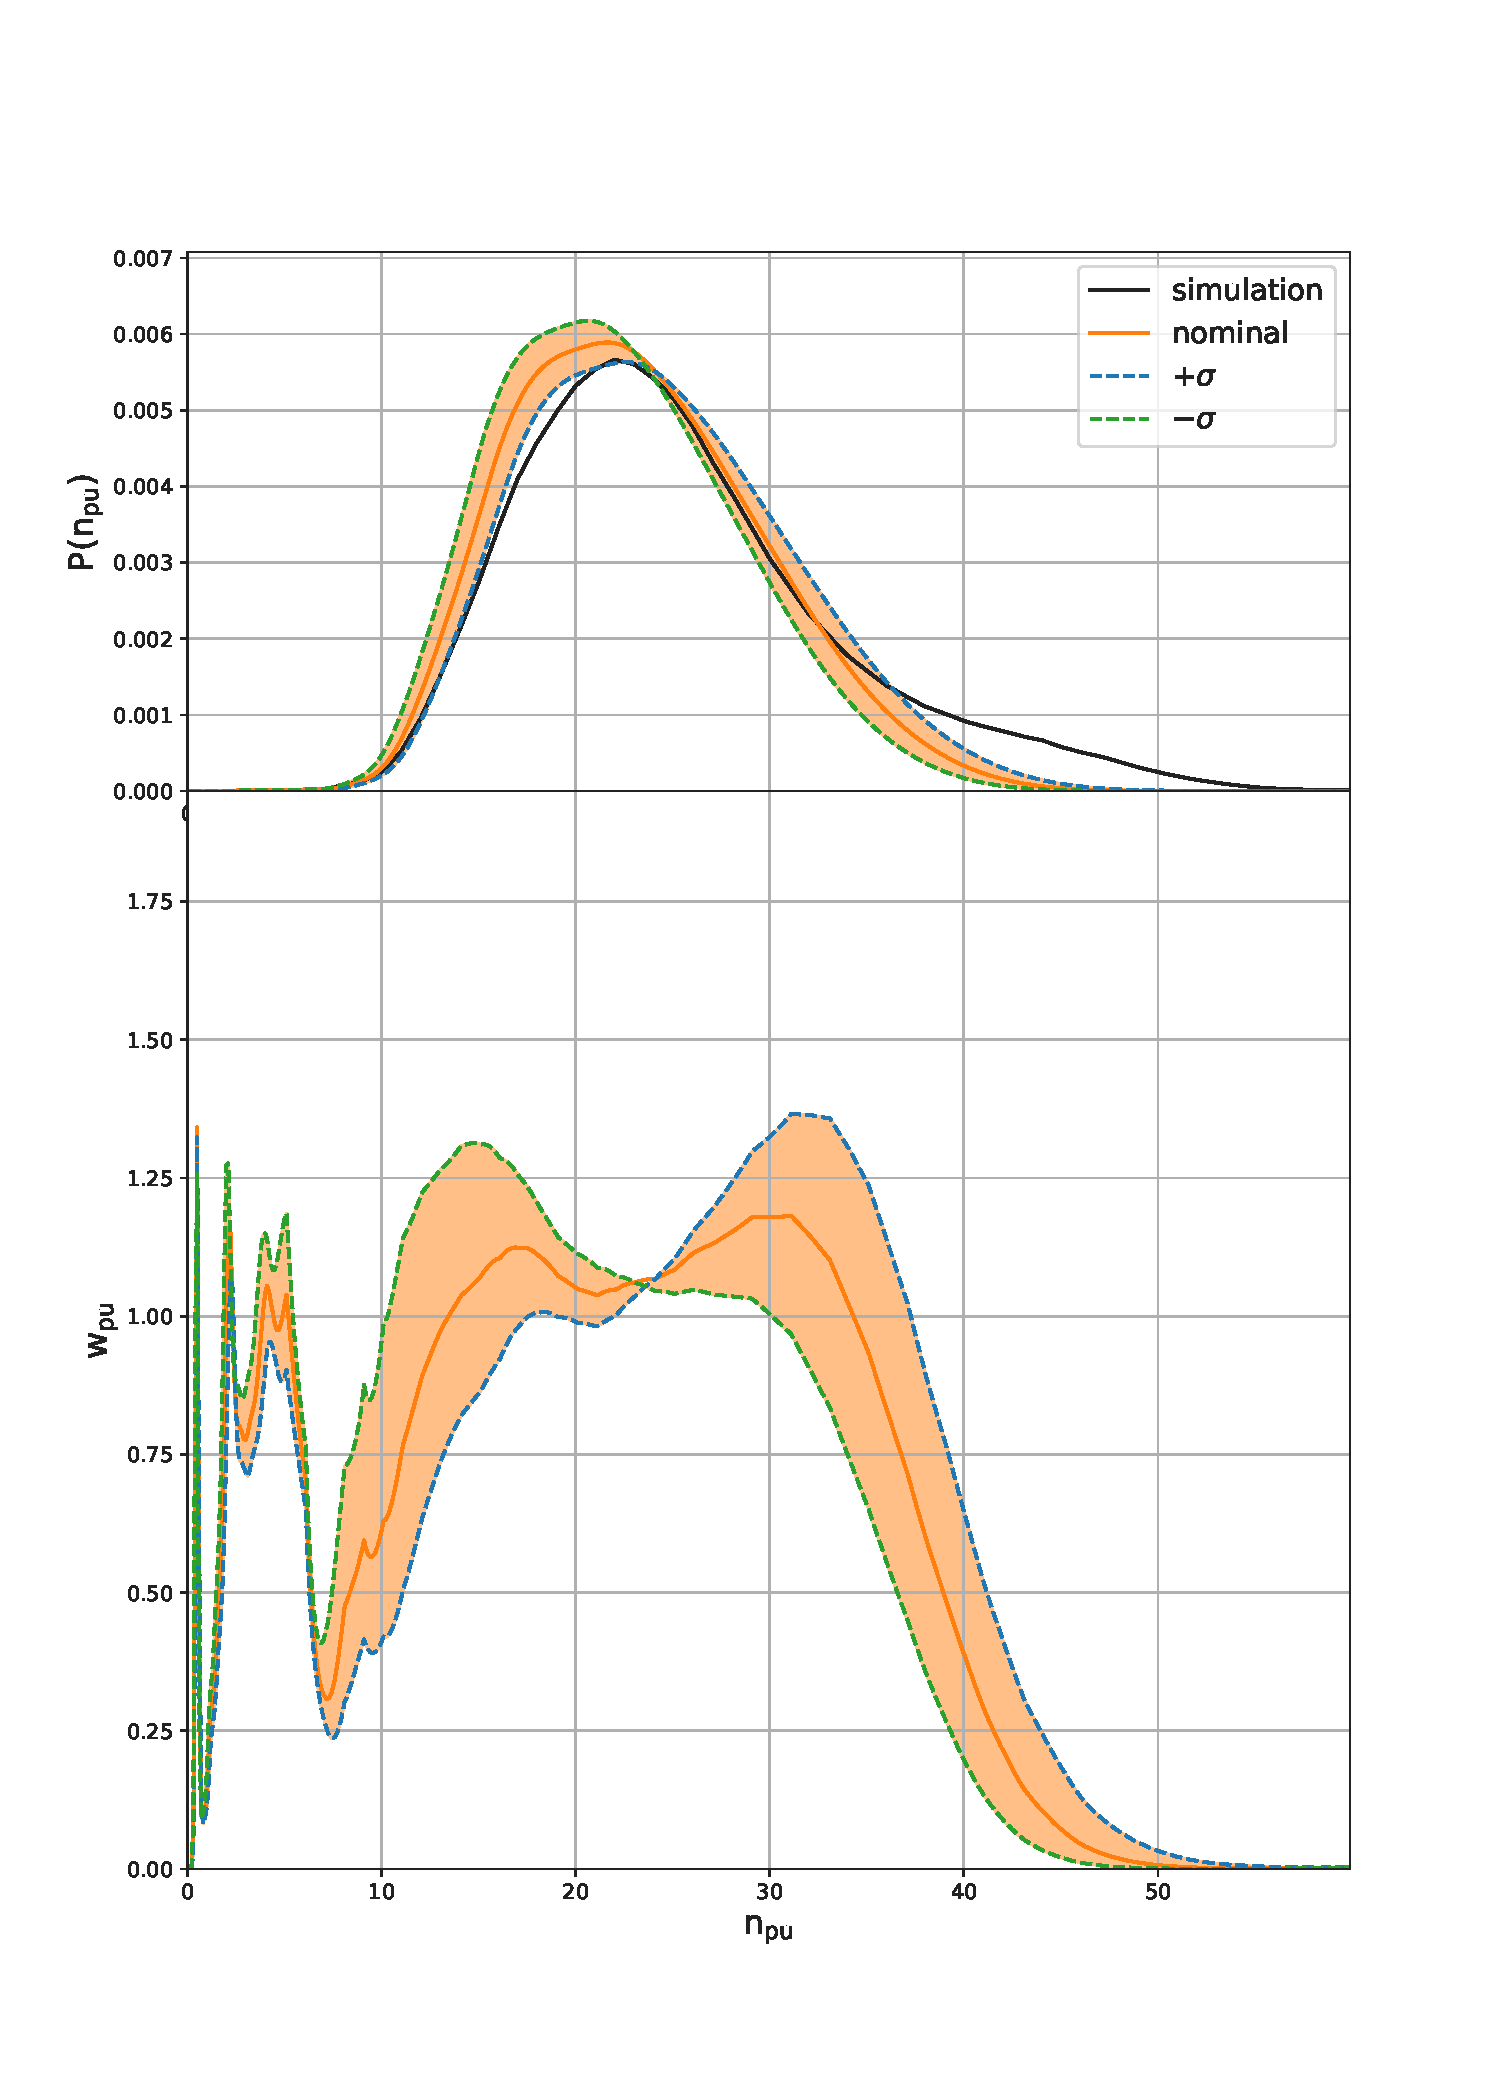
\includegraphics[height=0.4\textheight]{chapters/Analysis/sectionCalibration/figures/generator/pileup_systematics}
    % 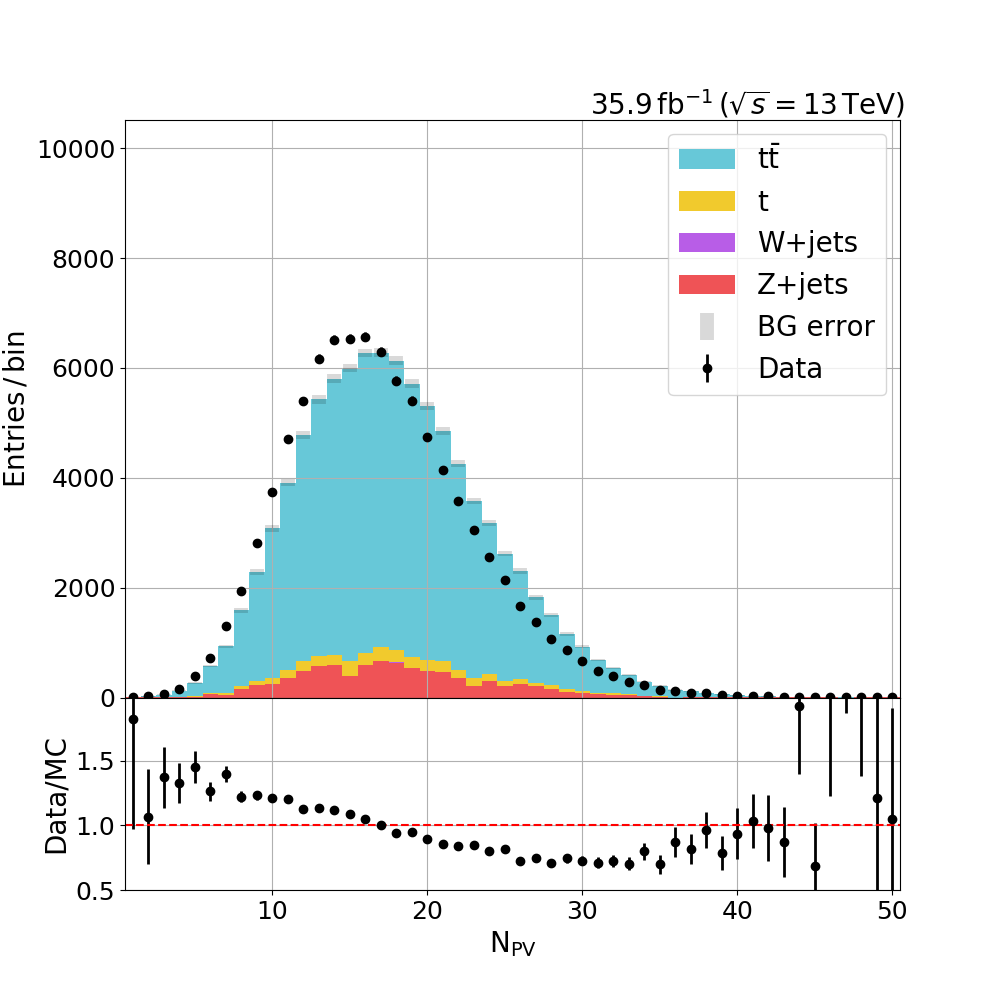
\includegraphics[height=0.4\textheight]{chapters/Analysis/sectionCalibration/figures/generator/n_pv}
    \caption{\emph{(top)} Pileup distribution in data and simulation including the $\pm\sigma$ variation of the data pileup distributions. \emph{(bottom)} The weights parameterized by number of simulated pileup resulting from taking the ratio of the pileup distribution in data and simulation. }
    % \emph{(right)} Comparison of primary vertex multiplicity between data and simulated datasets. }
    \label{fig:analysis:calibration:pileup}
\end{figure}
\FloatBarrier



%  top pt
\subsubsection{Top \pt Reweighting}
Additional corrections can be applied to the \ttbar sample to account for generator level mismodeling of the top quark \pt spectrum~\cite{CMS-PAS-TOP-16-011, CMS-PAS-TOP-16-008}.  This is done by identifying the parton-level top quarks, and calculating a scale factor from the equation, $SF_{\PQt}(\pt) = SF_{\PAQt}(\pt) = e^{0.0615-0.0005 \pt}$. The overall event weight is that is applied is $w = \sqrt{SF_{\PQt}SF_{\PAQt}}$.  We do not apply the weight, but instead use it as the systematical uncertainties associated with the top \pt correction.
\begin{figure}[ht]
    \centering
    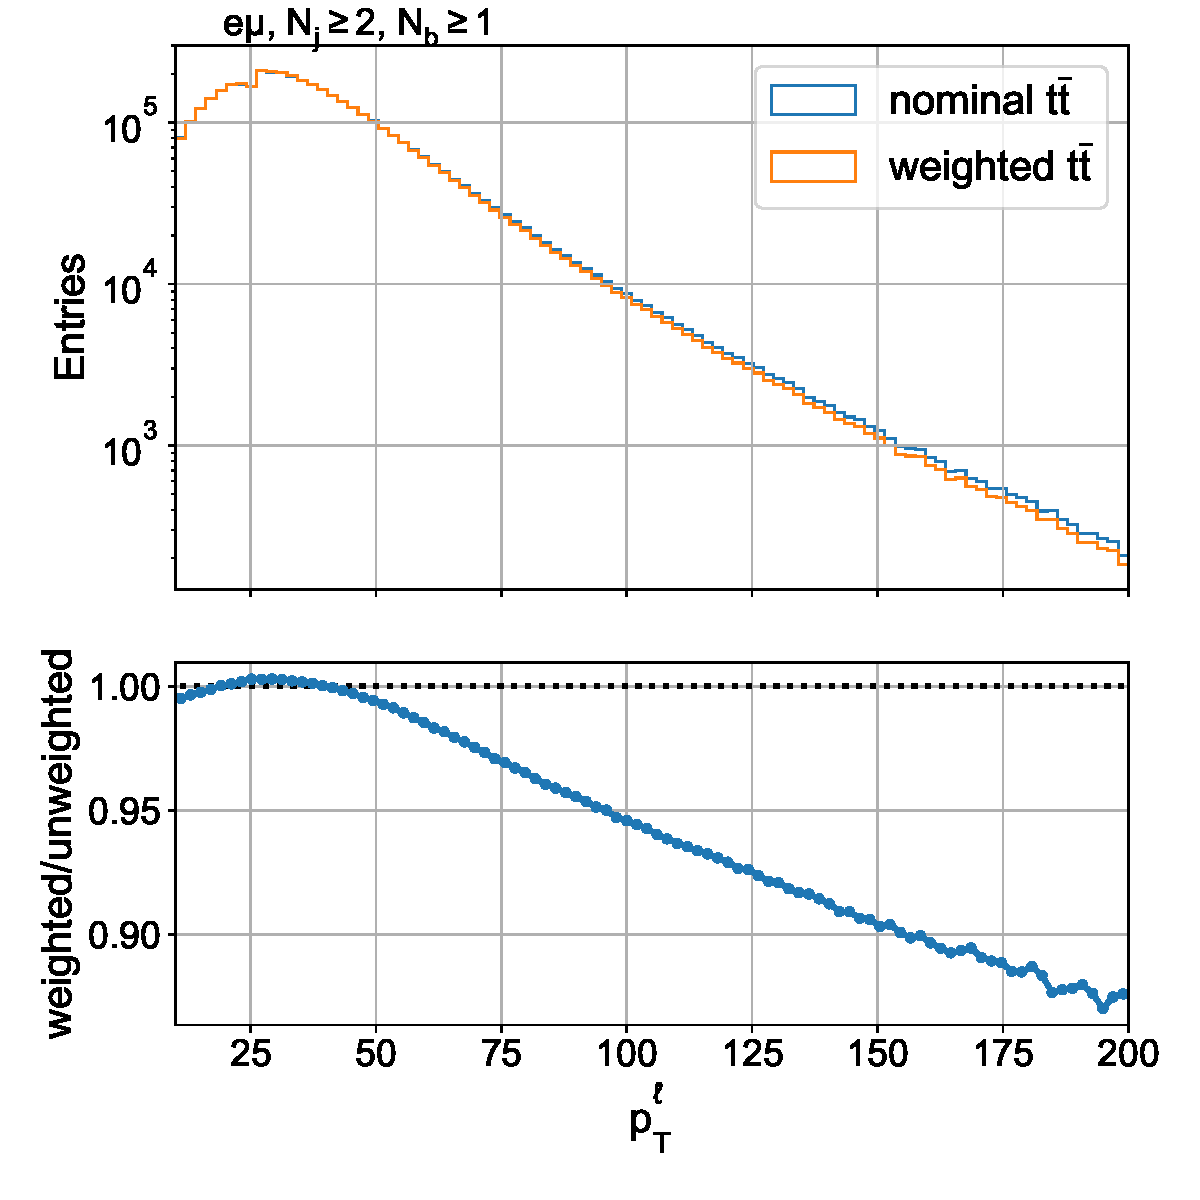
\includegraphics[width=0.55\textwidth]{chapters/Analysis/sectionCalibration/figures/generator/top_pt_weight}
    \caption{Comparison of the trailing lepton \pt distribution in $\cem$ events with at least two jets and at least one \PQb tag with top \pt weights applied and without the weights.}
    \label{fig:analysis:calibration:top_pt_weight}
\end{figure}


% z pt
\subsubsection{\PZ \pt  Reweighting}
Based on differences between the observed and predicted \PZ \pt spectrums, weights are derived to correct the \pt spectrum in simulation. The derivation of the weights was done in the context of the $\PH \rightarrow \WW $ analysis and is described in AN-2017-082. This correction does not have an associated uncertainty.
\begin{figure}[ht]
    \centering
    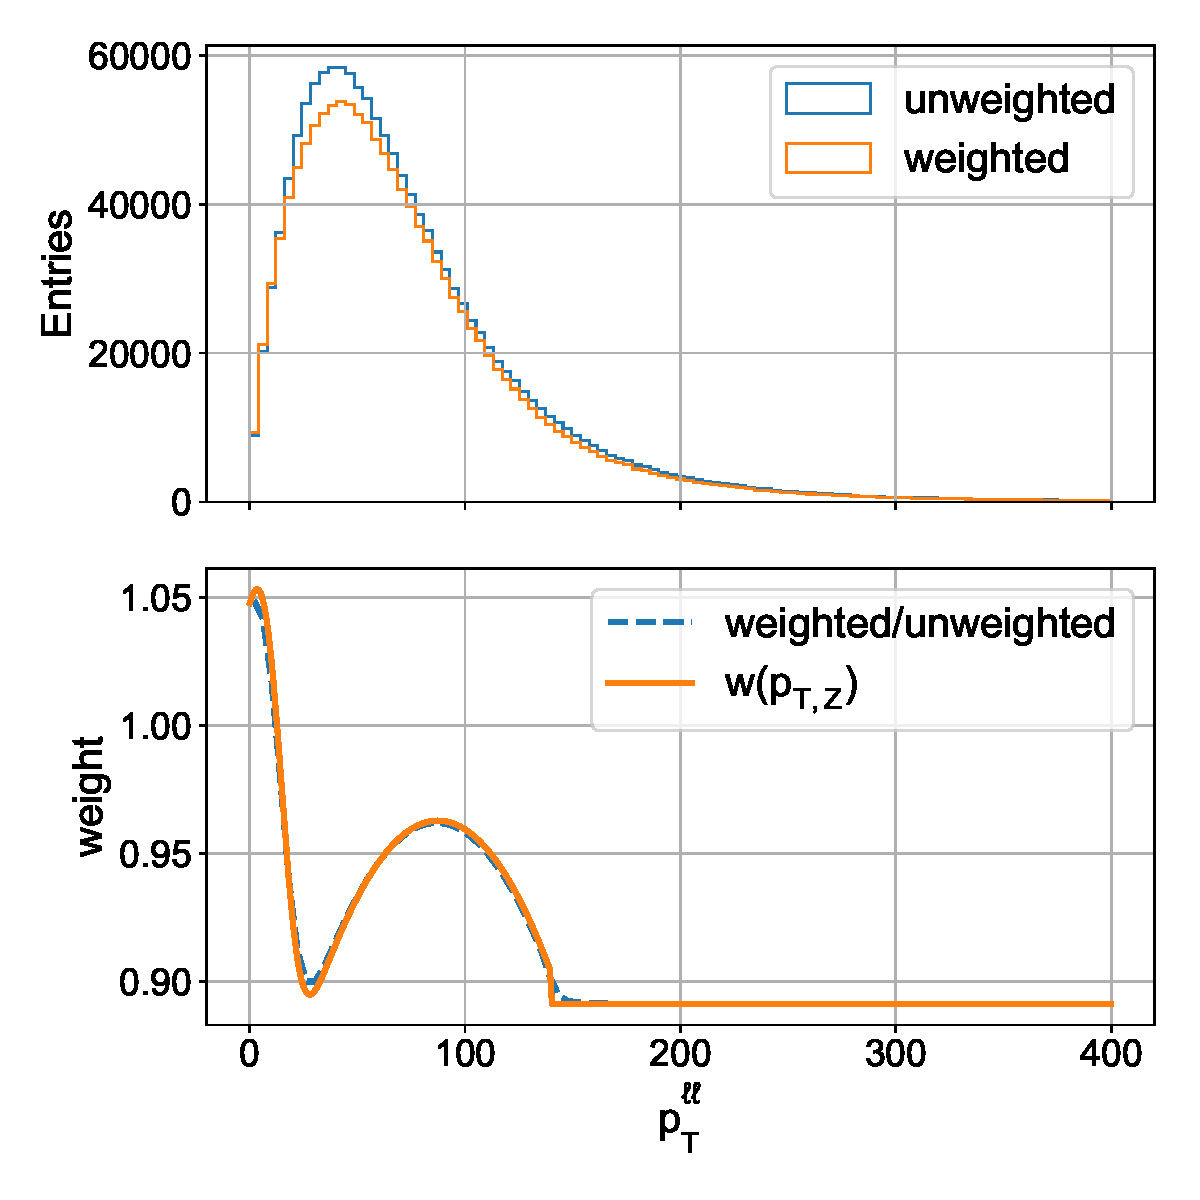
\includegraphics[width=0.55\textwidth]{chapters/Analysis/sectionCalibration/figures/generator/z_pt_weighting}
    \caption{\emph{(top)} Comparison of weighted and unweighted dilepton \pt spectrum for dimuon events with two jets and no \PQb tags. \emph{(bottom)} Comparison between ration of distributions in the top distribution and the analytical function for generating weights.}
    \label{fig:analysis:calibration:z_weight}
\end{figure}


% ww pt
\subsubsection{\WW \pt  Reweighting}
Estimation of the \WW process relies on the \POWHEG MC generator which is a NLO fixed order generator. Higher order corrections are therefore not directly included, but have been calculated separately~\cite{Meade:2014fca, Jaiswal:2014yba, Grazzini:2015wpa}.  The estimation of uncertainty is based on the description in AN-2017-273. As mentioned there, the theoretical uncertainty associated with the corrections have not been provided so they are estimated by varying the renormalization, factorization, and the matching scale of the \pt resummation technique. The weights and their systematic variations, as well as the effect on the lepton \pt spectrum in the \WW MC sample is shown in figure~\ref{fig:analysis:calibration:ww_weight}.

\begin{figure}[ht]
    \centering
    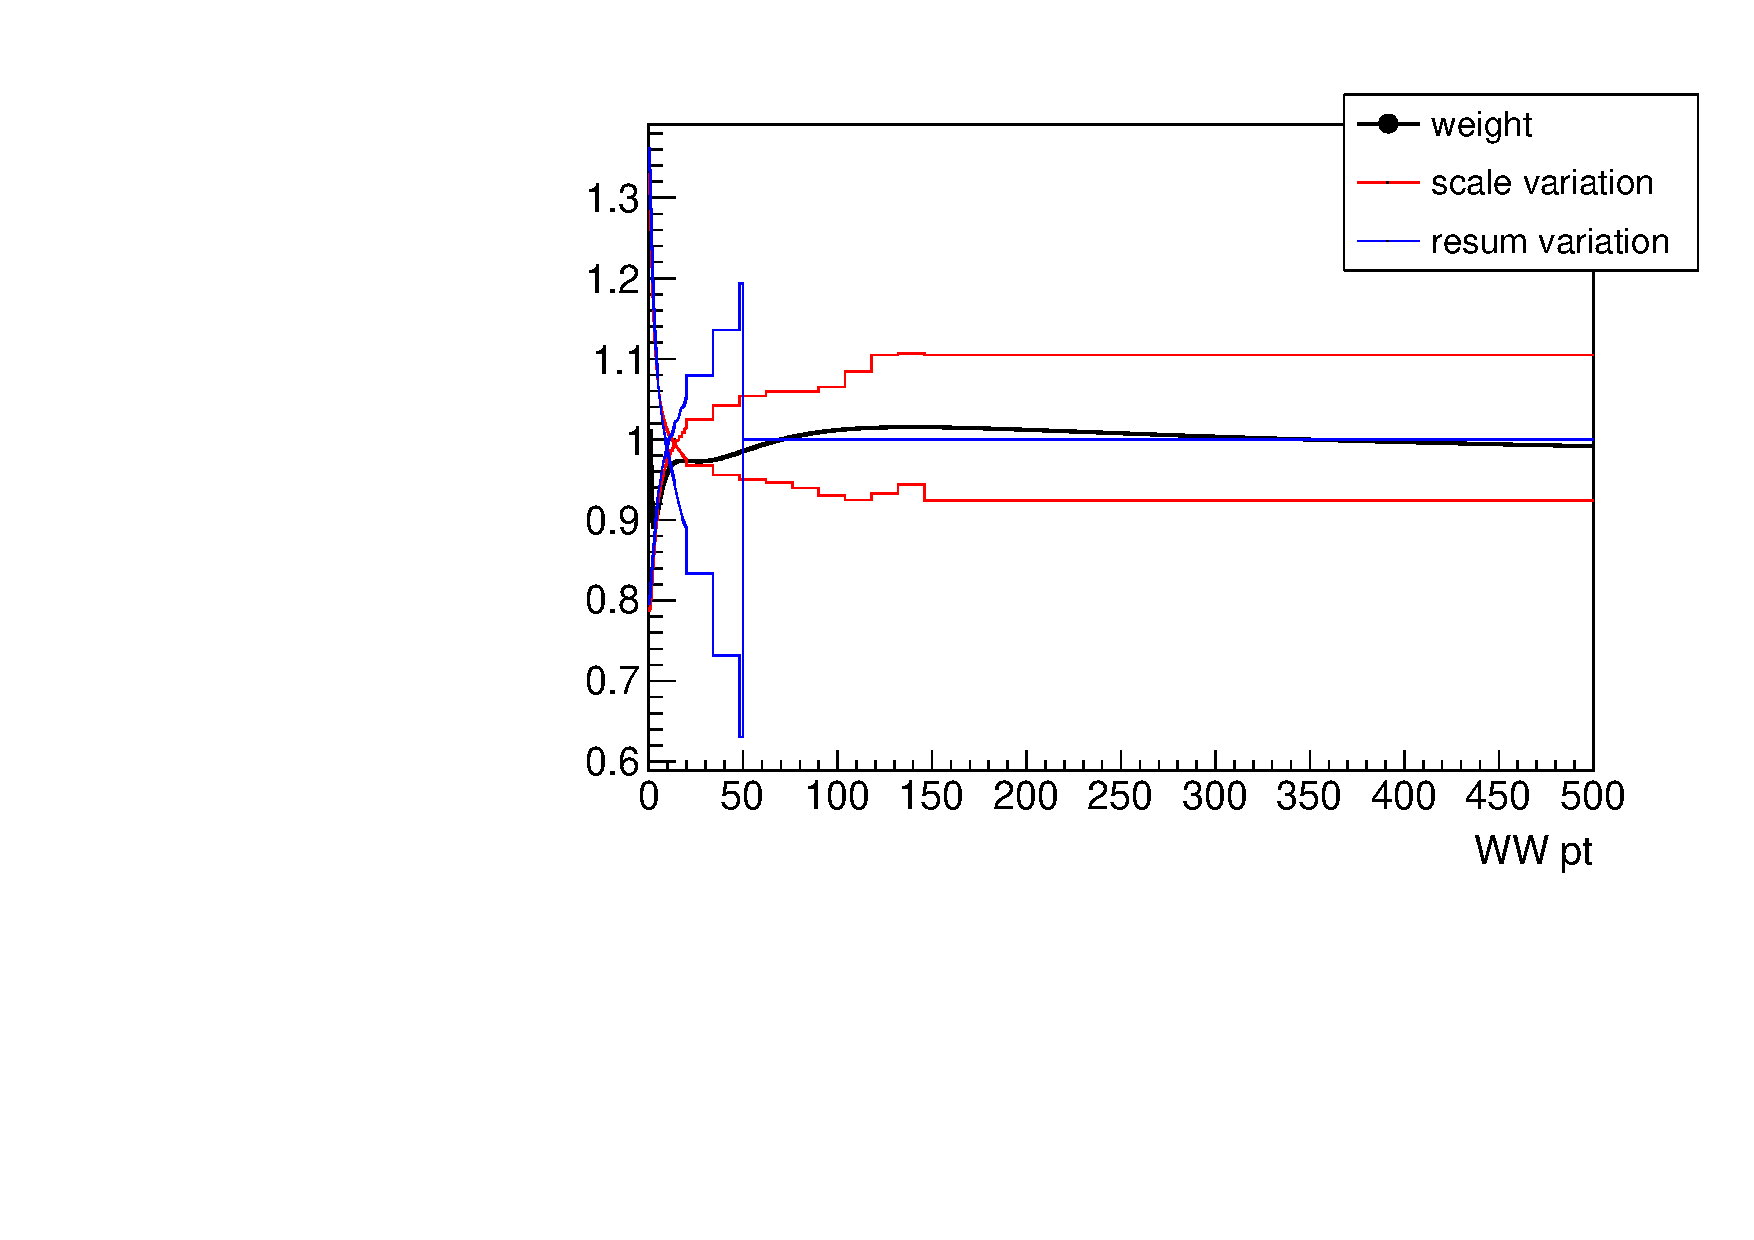
\includegraphics[width=0.5\textwidth]{chapters/Analysis/sectionCalibration/figures/generator/ww_pt_weight_variations}
    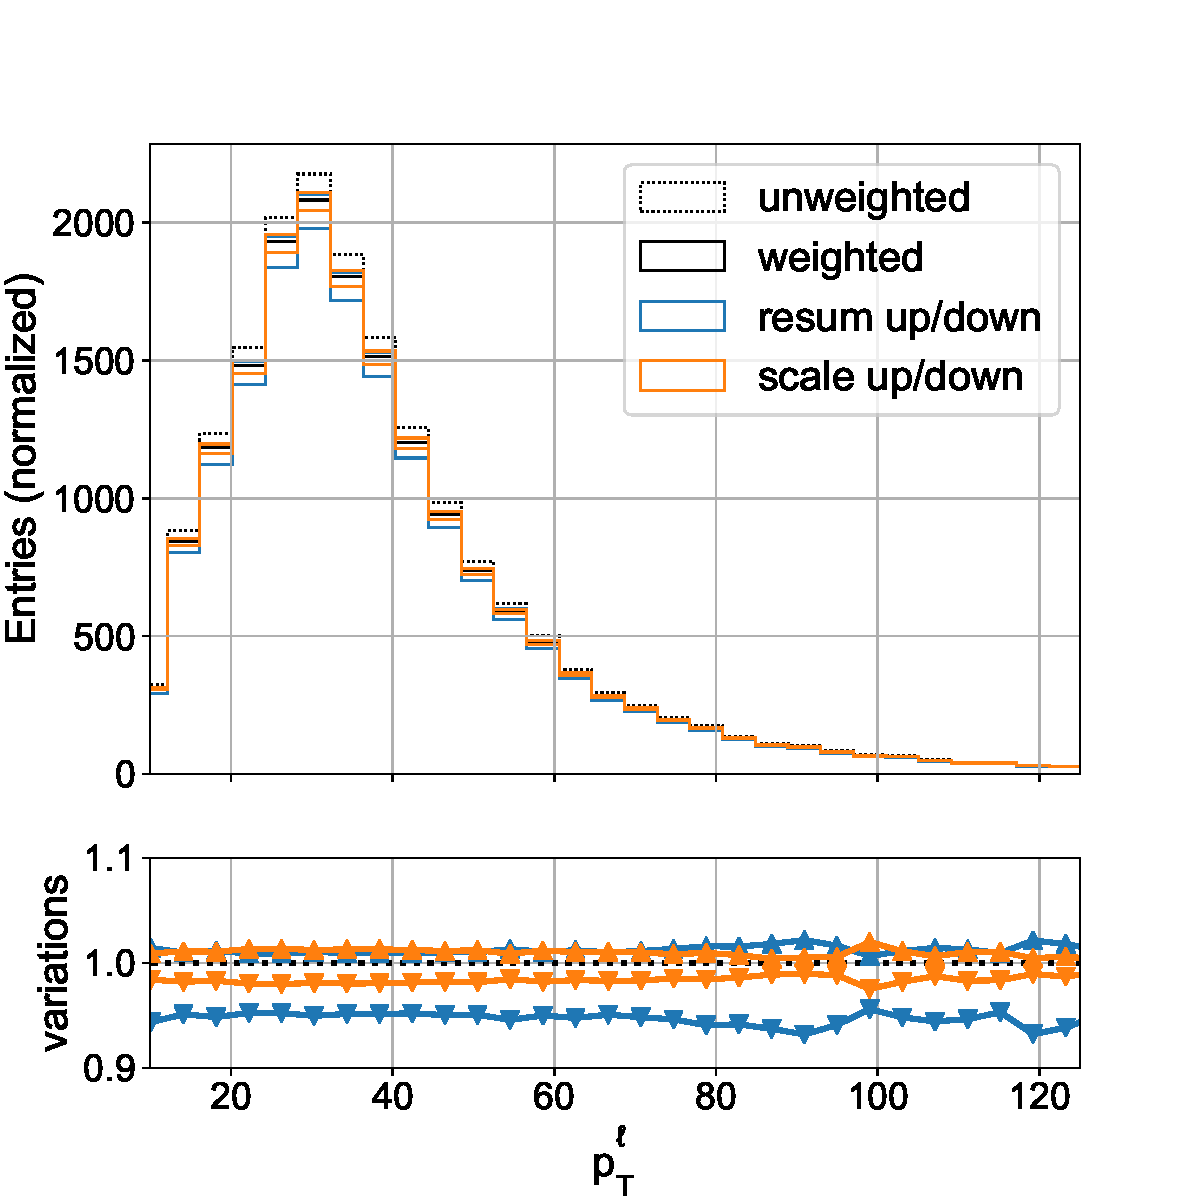
\includegraphics[width=0.38\textwidth]{chapters/Analysis/sectionCalibration/figures/generator/ww_pt_lepton_pt}
    \caption{\emph{(left)} Weights for the $\PQq \PQq \rightarrow \WW$ process as a function of the $\WW\,\pt$ and the two components of systematic variation.  \emph{(right)} Trailing lepton pt from the $\PQq \PQq\rightarrow \WW\rightarrow \cem\PGn\PGn$ simulated sample when there are no reconstructed jets.} 
    \label{fig:analysis:calibration:ww_weight}
\end{figure}




\FloatBarrier




\subsection{Corrections for Physics Objects}
\label{sec:analysis:calibration:objects}

The some of the standard calibrations for the physics objects are provided by POGs and are applied to the selected objects in this analysis to account for potential mismodeling of the reconstruction and selection of physics objects in the simulation.
\subsubsection{Muons} 
Muons in the simulation are corrected for the energy scale, identification, and isolation efficiencies.

\subsubsection{Electrons} 
Electrons are corrected for the energy scale and resolution, reconstruction, and isolation efficiencies.

\subsubsection{Hadronic Taus} 
The scale factor accounting for the difference of tau identification efficiencies in the simulation and data were measured in several control regions~\cite{CMS-TAU-16-003-001}.  The measurement is carried out in both in two different control regions: one enriched in $\PZ\to\PGtl\PGth$ production and one enriched in \ttbar.  Because of the large overlap with our signal region in the case of the latter, the former measurement is used so that the datasets that are used are uncorrelated.  For the selection algorithm and tight working point a scale factor of $0.95 \pm 0.05$ is used; for the very tight working point it is $0.92 \pm 0.05$. The scale factors accounting for difference of tau energy in the  simulation and data are measured by fitting to the sensitive variables. This energy correction is split into different \PGth decay modes.  Two sensitive variables are considered. One is the visible mass $m_{\rm vis}$ of the \cet or \cmt in the $\PZ\to\PGt\PGt$ region, the other is the visible mass of hadronic taus $m_\PGth$ ~\cite{CMS-TAU-16-003-001}. In this analysis, the energy scale factors measured with the former are applied to correct the simulation. The values of energy scale factors are
\begin{equation*}
    \PGt \to \mathrm{h}^{\pm}:0.995(5), \quad \PGt \to \mathrm{h}^{\pm}\PGpz:1.011(3), \quad \PGt \to \mathrm{h}^{\pm}\mathrm{h}^{\mp}\mathrm{h}^{\pm}\PGpz:1.006(3)
\end{equation*}
\noindent Also corrections for $j\to \PGth$ misidentification is applied, which is measured by us in a $j\to \PGth$ fake-enriched region. More details about the measurement is presented in Section~\ref{sec:analysis:calibration:jetToTauh}.


\subsubsection{Jets and $\mathrm{b}$ tags}
The measurement of jet energy in the detector has a small offset and spread comparing with the ground-truth of the original seeding gluons or quarks because of the noisy hadronic and pile-up environment and the nature of detector response. This effect is accounted for by the jet energy scale (JES) and jet energy resolution (JER).

To account for the difference in \PQb tag efficiency in data and simulation, the \PQb tag status of jets is modified based on a set of scale factors derived by the \PQb tag POG.  The method used for applying the \PQb tag scale factors modifies the status of individual jets to either promote or demote their \PQb tagging status~\cite{twiki:btag_method}.  The method relies on the user measuring the \PQb tag efficiencies and mistag probabilities in the simulated samples.  This is described further in Section~\label{sec:analysis:calibration:btag}.








\subsection{Corrections for Trigger Efficiencies}
\label{sec:analysis:calibration:trigger}


\subsubsection{Single Muon Trigger}
The corrections of the single muon trigger efficiencies \texttt{HLT\_IsoMu24} are applied as event weights calculated based on the presence of triggering muons in \cme, \cmm, \cmt, \cmh channels. The scale factors are defined as the ratio between trigger efficiencies in the data over the efficiencies in the simulated dataset, and have a dependence on \pt and $|\eta|$. Muon POG provides the scale factors for two separated periods, 2016 BCDEF and GH, shown in Figure~\ref{fig:analysis:calibration:mu24TriggerSF}.
\begin{figure}
    \centering
    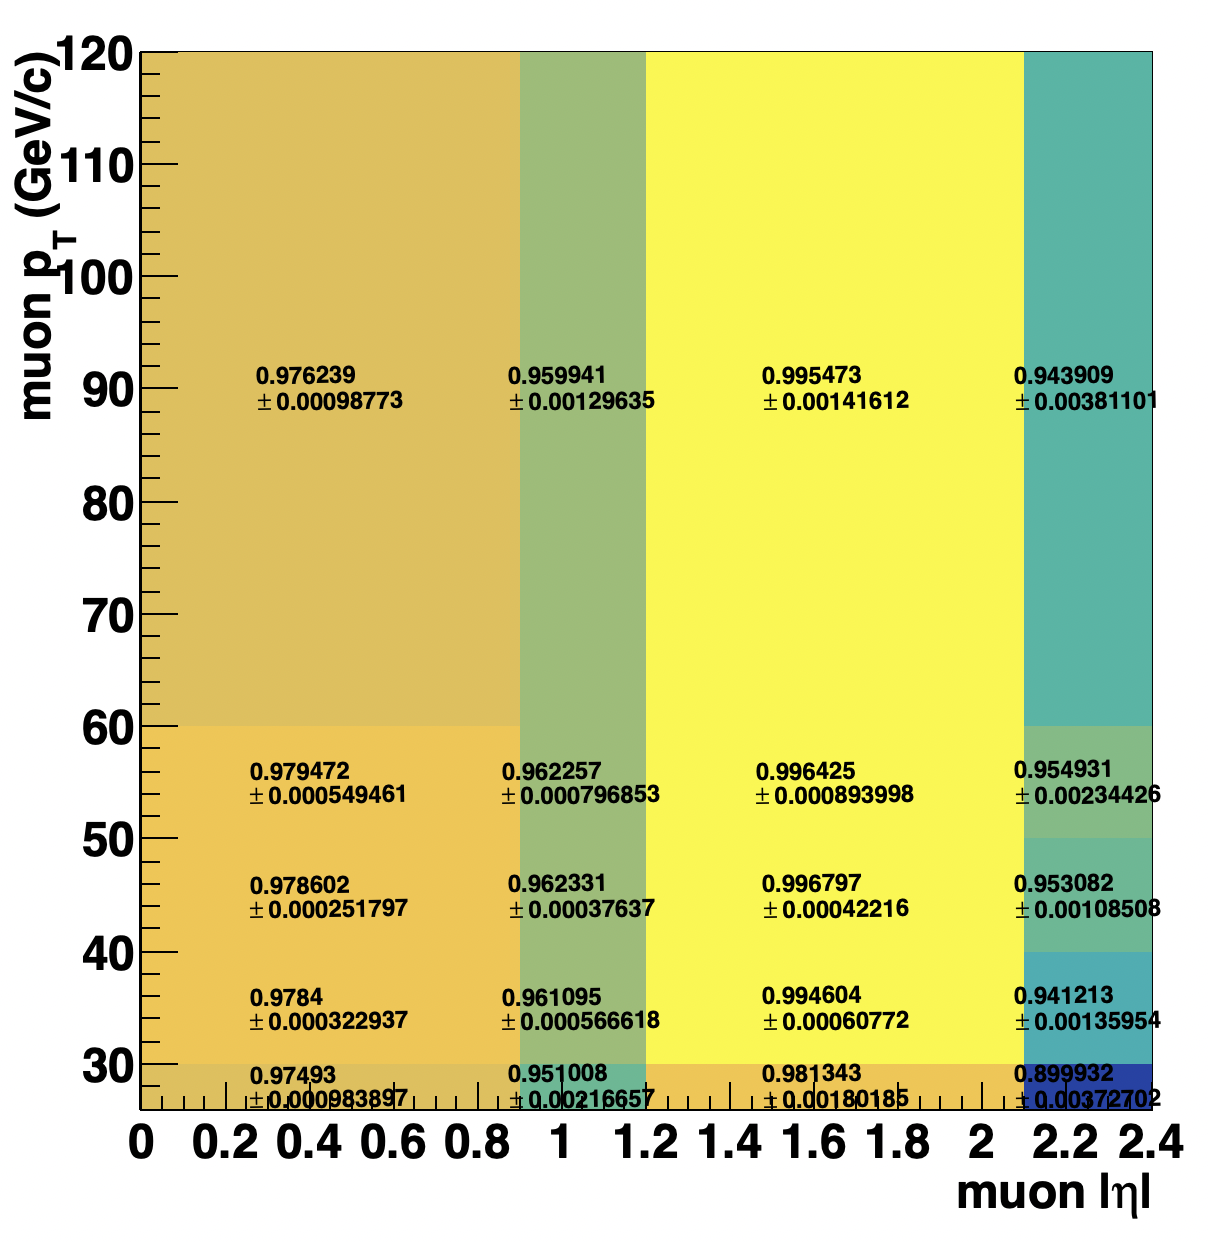
\includegraphics[width=0.45\textwidth]{chapters/Analysis/sectionCalibration/figures/trigger/muTrSF_BCDEF.png}
    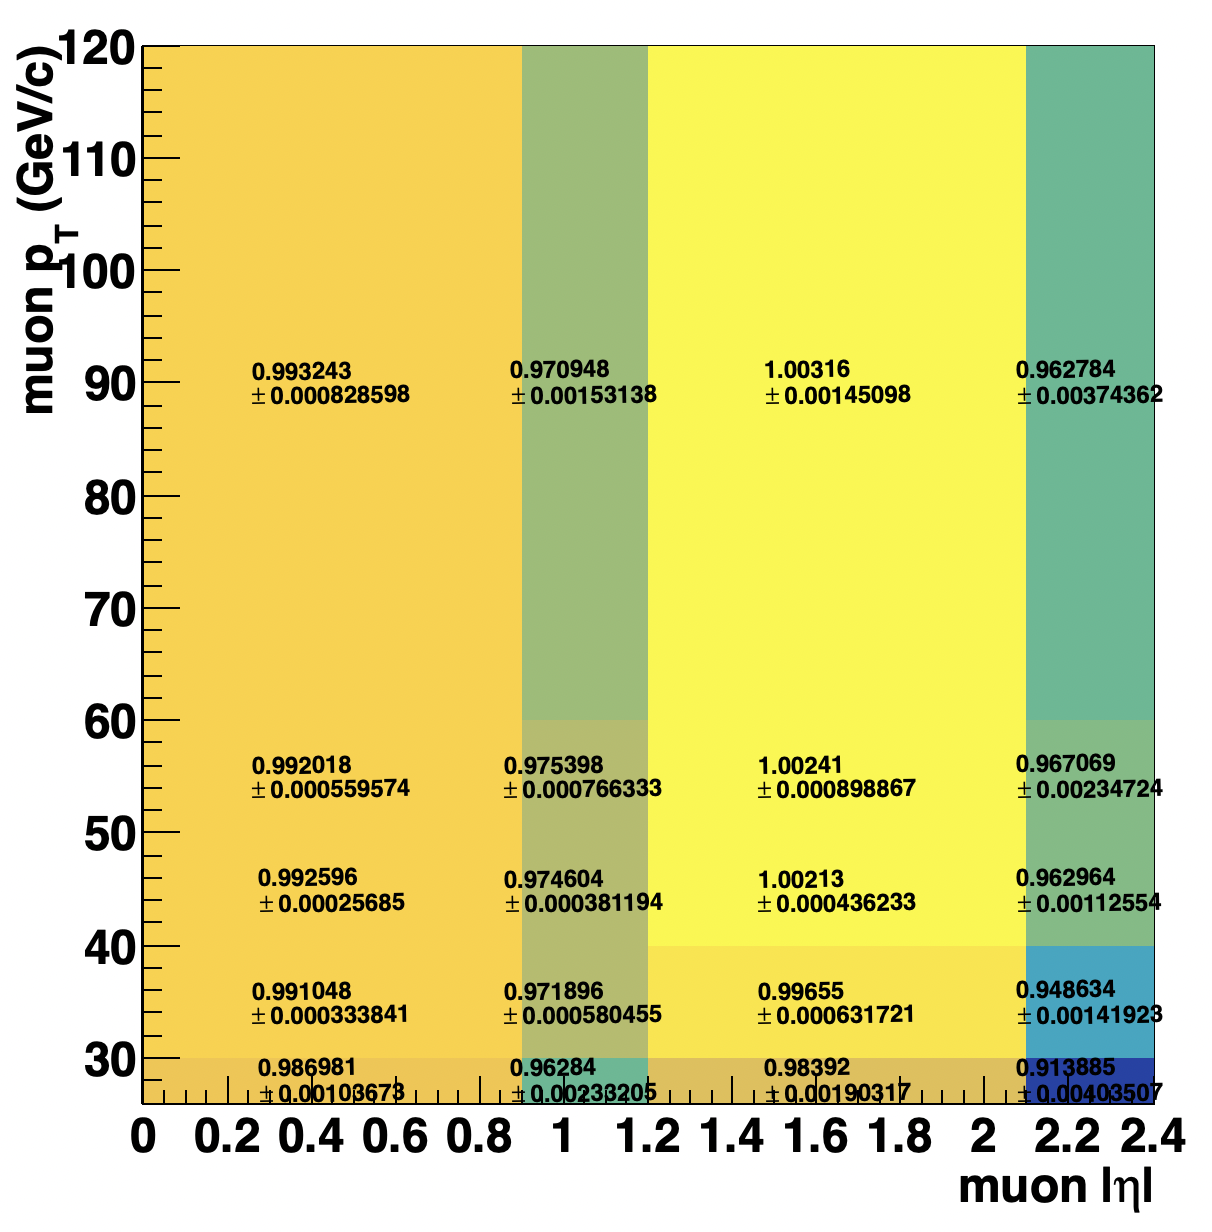
\includegraphics[width=0.45\textwidth]{chapters/Analysis/sectionCalibration/figures/trigger/muTrSF_GH.png}
    \caption{Scale factors for the single muon trigger efficiencies in run periods 2016 BCDEF \emph{(left)} and GH \emph{(right)}. The uncertainties displayed are only statistical uncertainties.}
    \label{fig:analysis:calibration:mu24TriggerSF}
\end{figure}





\subsubsection{Single Electron Trigger}
% selection
The correctons of the single electron trigger efficiencies \texttt{HLT\_Ele27\_WPTight\_Gsf} are applied as event weights calculated based on the presence of triggering electrons in \cee, \cem, \cet, \ceh channels. The scale factors are defined as the ratio between trigger efficiencies in the data over the efficiencies in the simulated dataset, and have a dependence on \pt and $|\eta|$. Thought EGamma POG provides the scale factors, but the uncertainties associated to the measurement are not included. In order to better account for the uncertainties of the scale factors, we have performed a dedicated measurement using the standard tag-and-prob approach recommended by the EGamma POG.
\begin{figure}
    \centering
    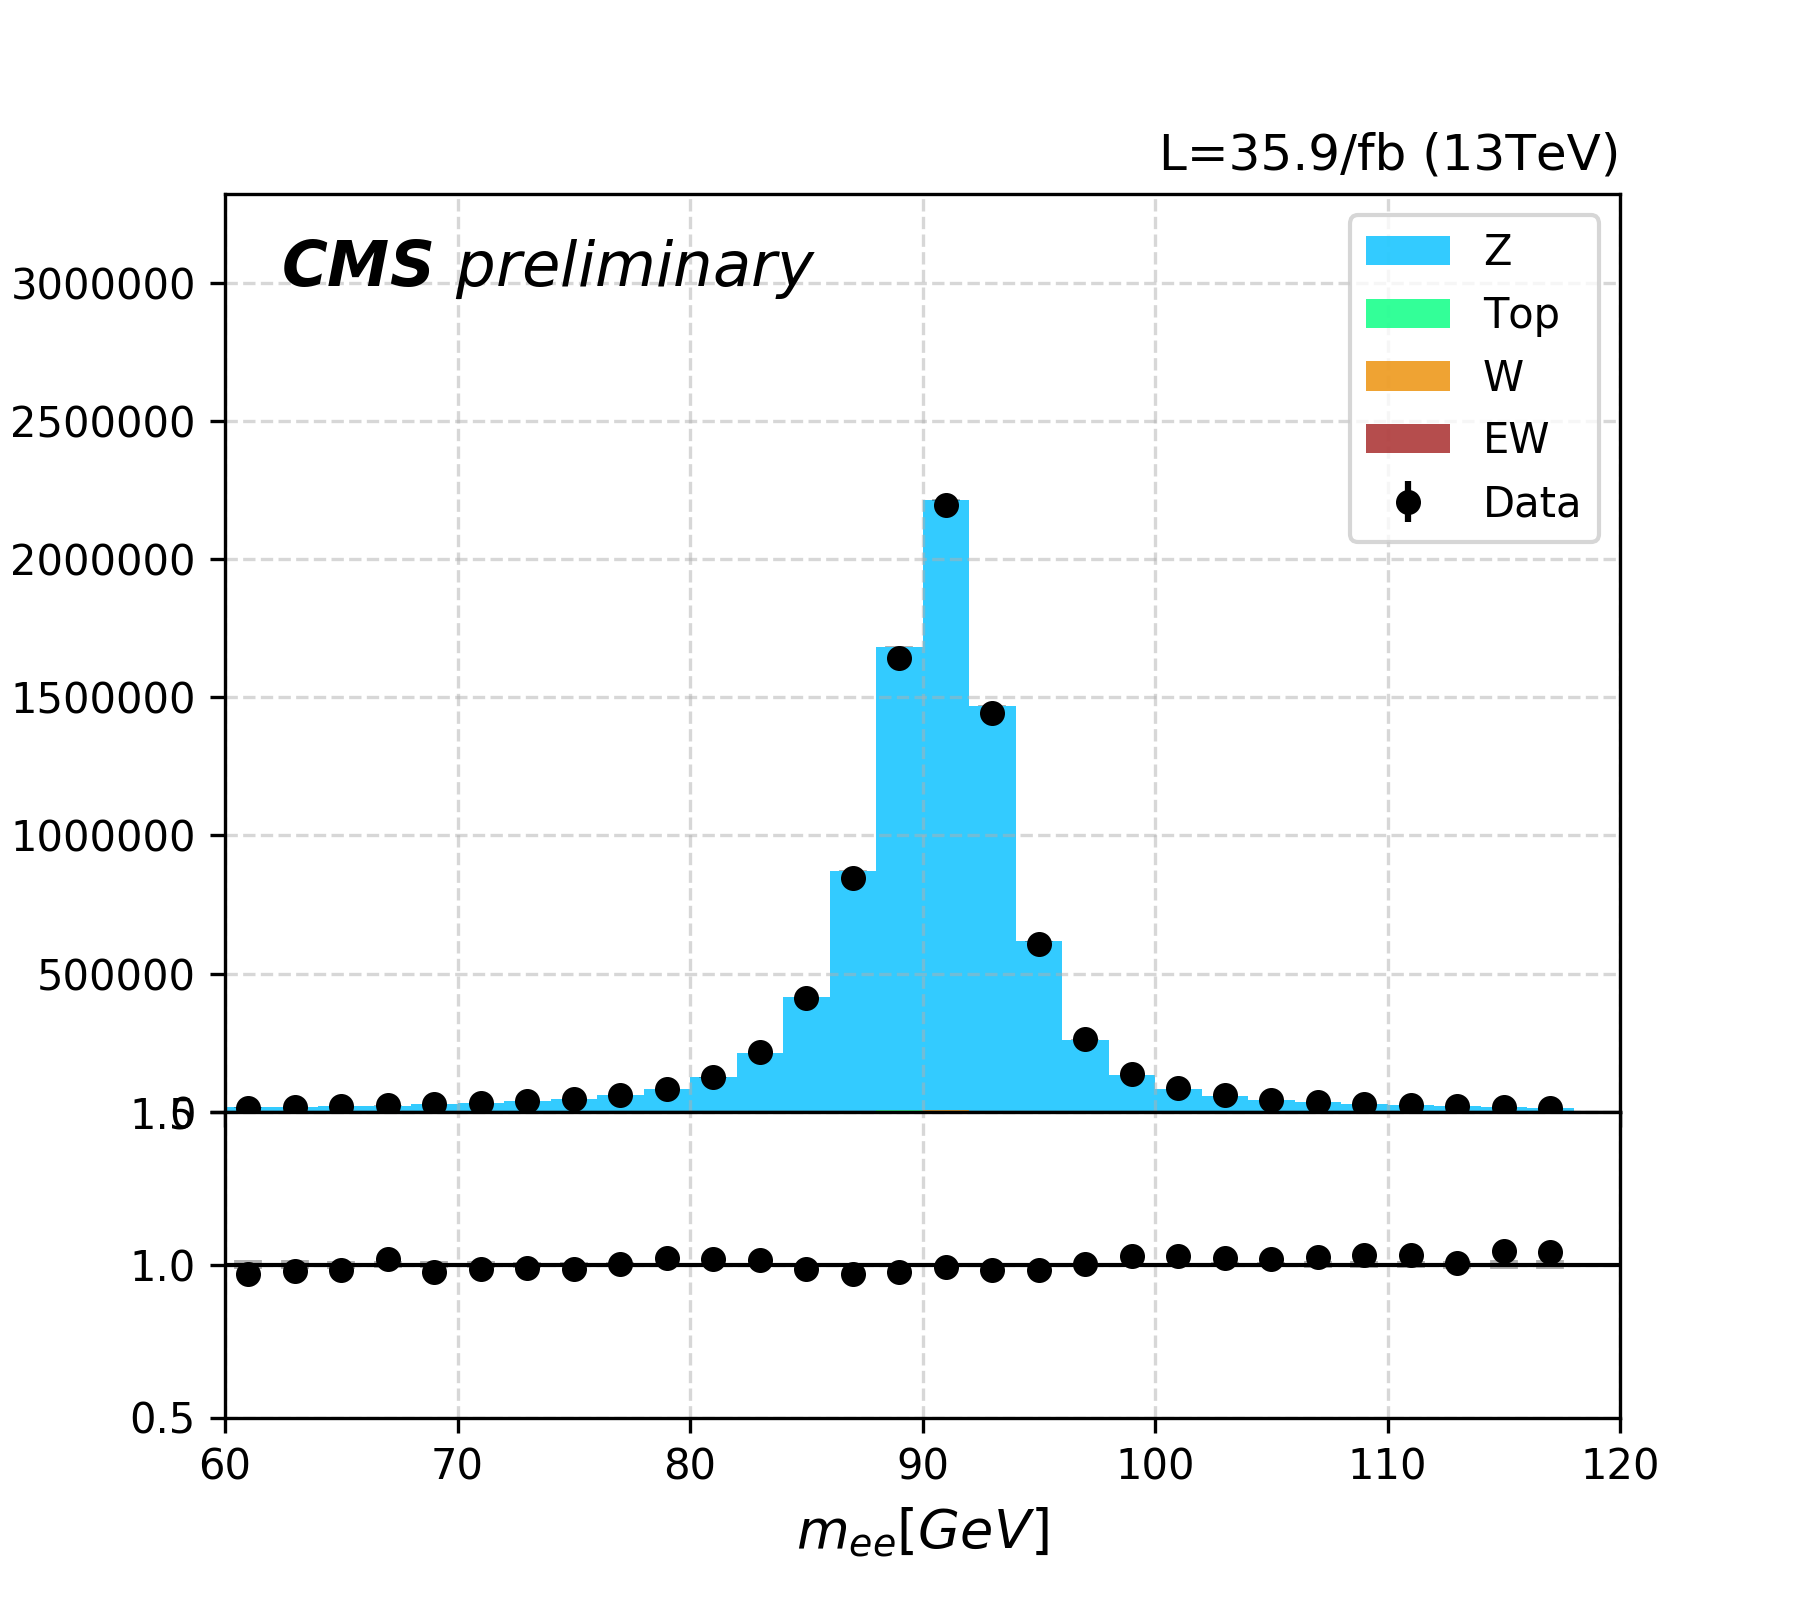
\includegraphics[width=0.5\textwidth]{chapters/Analysis/sectionCalibration/figures/eTrigger/dileptonMass_tag30.png}
    \caption{The $m_{\cee}$ distribution of the selected events for the measurement of the scale factors of single-electron trigger efficiencies.}
    \label{fig:analysis:calibration:mass_ee}
\end{figure}
In our SF measurement, the dataset used  is 2016 re-reco \texttt{SingleElectron} dataset with the golden certificate luminosity mask, while the simulations include \texttt{DYJETSToLL\_M-10to50\_amcatnlo}, \texttt{DYJETSToLL\_M-50\_amcatnlo} and \texttt{TT\_powheg}, reweighted to pile-up $\sigma_{\rm mb} = 69.2\pm 2.3$ nb. The electrons are selected with tight identification and tight particle-flow isolation with $\pt>20\GeV$ and $|\eta|<2.5$. Among selected electrons, tagged electrons are defined as $\pt>30\GeV$ and outside gap between barrel and endcap calorimeter $1.444<|\eta|<1.56$, and match with \texttt{HLT\_Ele27\_WPTight\_Gsf} triggering objects. Events are selected by requiring exactly 2 opposite electrons with at least 1 tagged electron and $60<m_{\cee}<120 \GeV$. This event selection yields a sample of events significantly dominated by Drell-Yan (DY)  process. The distribution of $m_{\cee}$ is shown in fig~\ref{fig:analysis:calibration:mass_ee}, where it can be seen that the purity of DY is very high in the selected \cee events. Thus a signal-backgound fit is not necessary to get DY yields.
% tag-prob
In each event, if one electron is tagged, the other consequently become a prob. Each event provides either one or two tag-prob pairs. A prob is passing if it match with \texttt{HLT\_Ele27\_WPTight\_Gsf} triggering objects. The trigger efficiencies are calculated by the ratio between the number of passing probs over the total probs in $\pt-\eta$ bins, 
\begin{equation*}
    \epsilon (\pt, \eta) = \frac{ N_{\rm passing} (\pt, \eta) } {  N_{\rm total} (\pt, \eta) }.
\end{equation*}
\noindent The scale factors are defined as the ratio between efficiencies in the data over efficiencies in the simulation,
\begin{equation}
SF (\pt, \eta) = \frac{\epsilon_{\rm{Data}} (\pt, \eta) }{\epsilon_{\rm{Simulation}} (\pt, \eta) }.
\end{equation}
\noindent The measurement of the scale factors is divided for two run periods, 2016 BCDEF and GH. This is because in run 2016 BCDEF,  the triggering efficiencies in the endcap suffers from a decrease of signal over noise ratio associated to the loss of tracking hits caused by problems in the pre-amplifier of the readout chips in the tracker's silicon microstrips. In the mid August 2016, this problem of Si-strip in endcap region is fixed by increase the drain speed of the pre-amplifier. Thus the trigger efficiencies were improved in run 2016 GH. For the two run periods, Figure~\ref{fig:analysis:calibration:ele27SF} shows the measured $\epsilon_{\rm{data}}$, $\epsilon_{\rm{MC}}$ and $SF$. The $SF$ for individual run periods are shown in Figure~\ref{fig:analysis:calibration:ele27SFperiods}, where a clear improvement can be seen in period G with respective to period F.
\begin{figure}
    \centering
    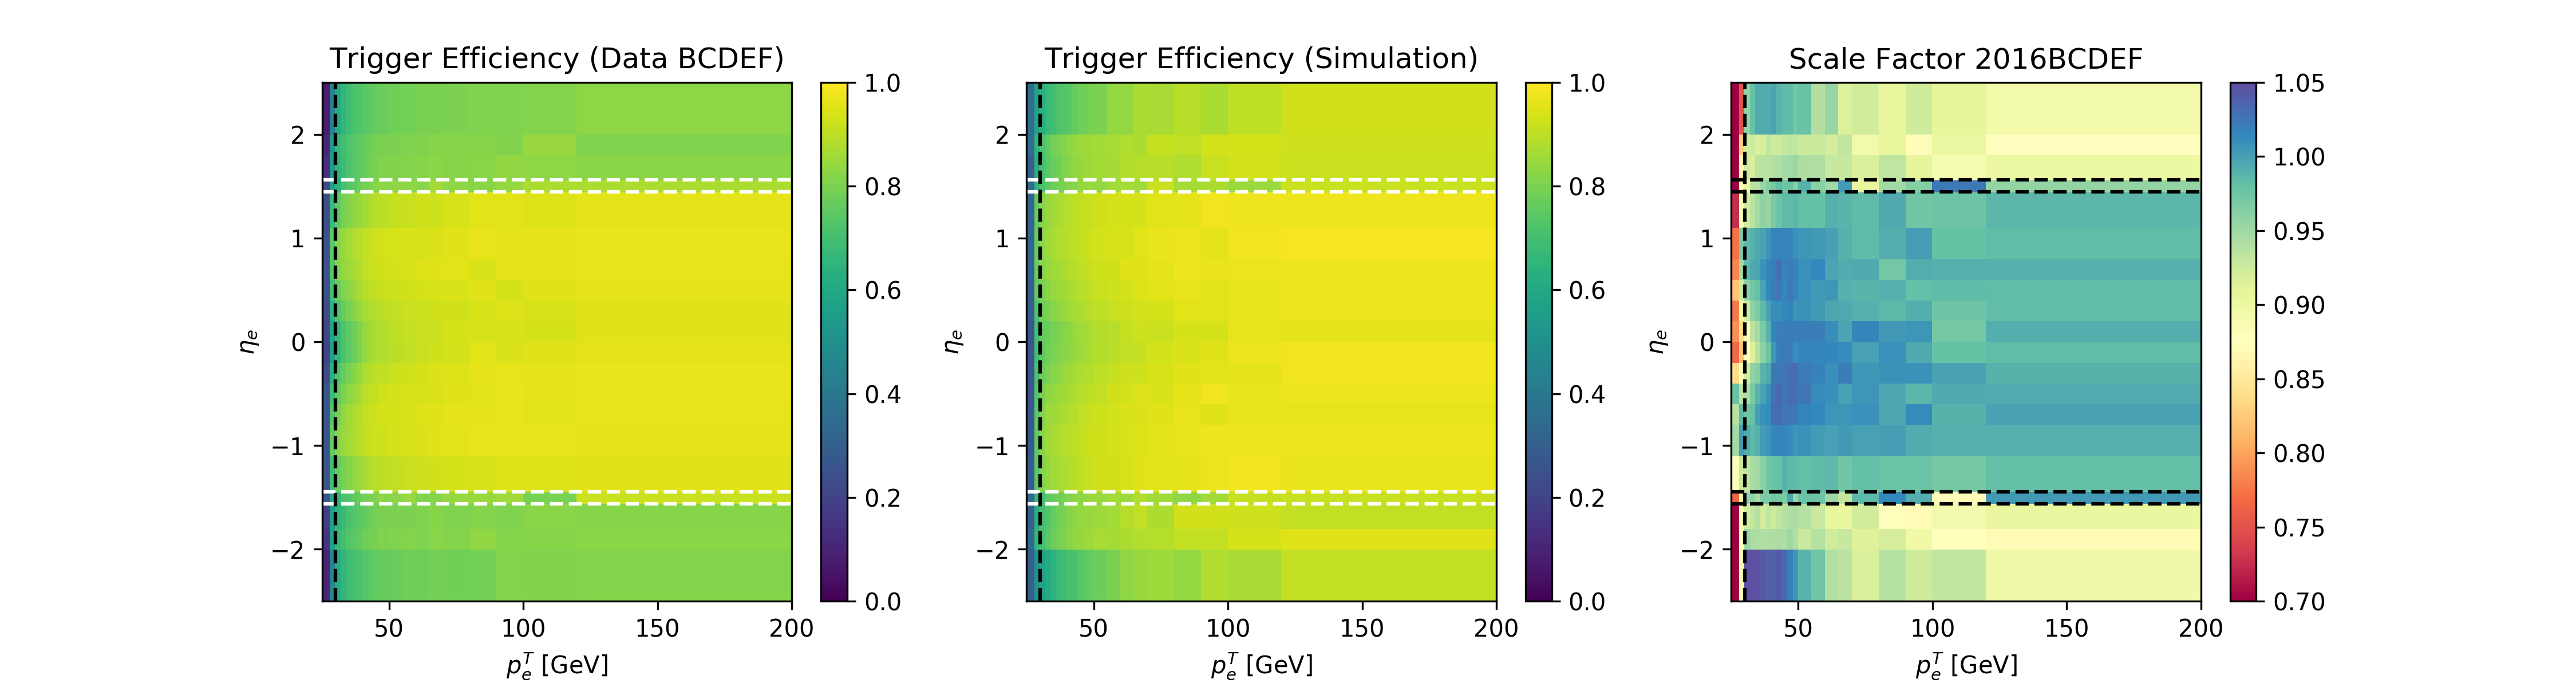
\includegraphics[width=0.99\textwidth]{chapters/Analysis/sectionCalibration/figures/eTrigger/eff2d_BCDEF.png}
    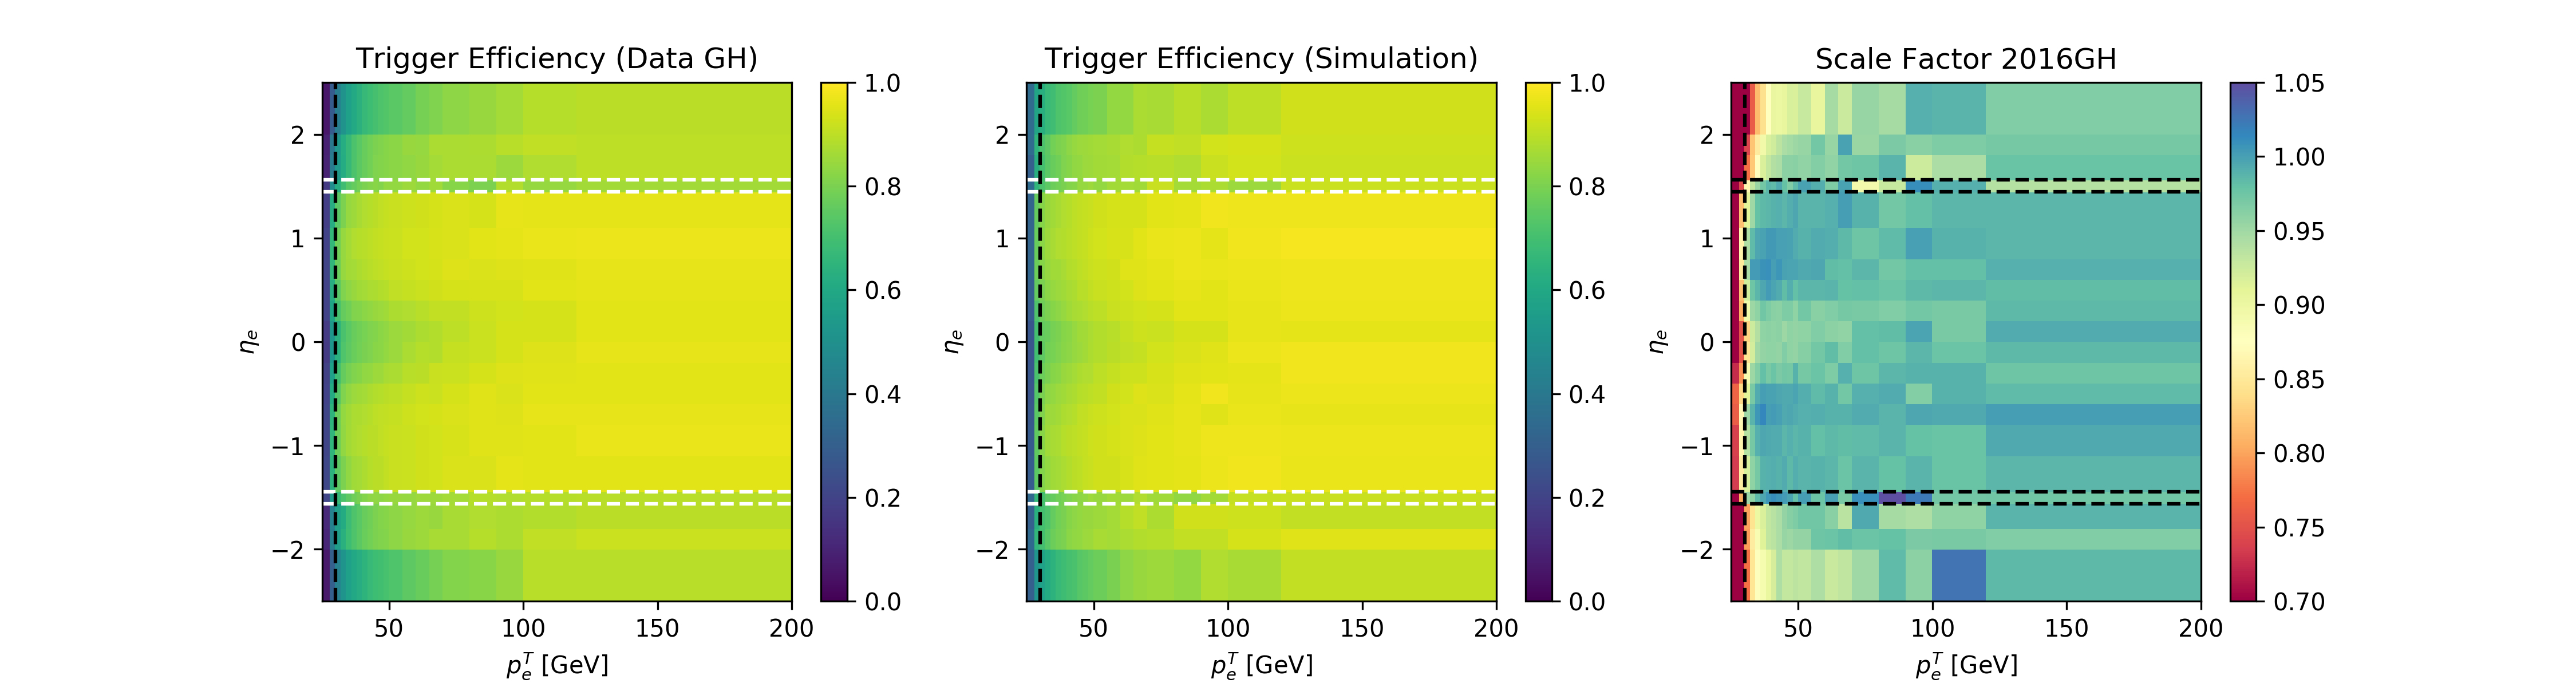
\includegraphics[width=0.99\textwidth]{chapters/Analysis/sectionCalibration/figures/eTrigger/eff2d_GH.png}
    \caption{The 2D maps of $\epsilon_{\rm{data}}$, $\epsilon_{\rm{MC}}$ and scale factors in run period 2016 BCDEF \emph{(upper)} and 2016 GH \emph{(lower)}.}
    \label{fig:analysis:calibration:ele27SF}
\end{figure}
\begin{figure}
    \centering
    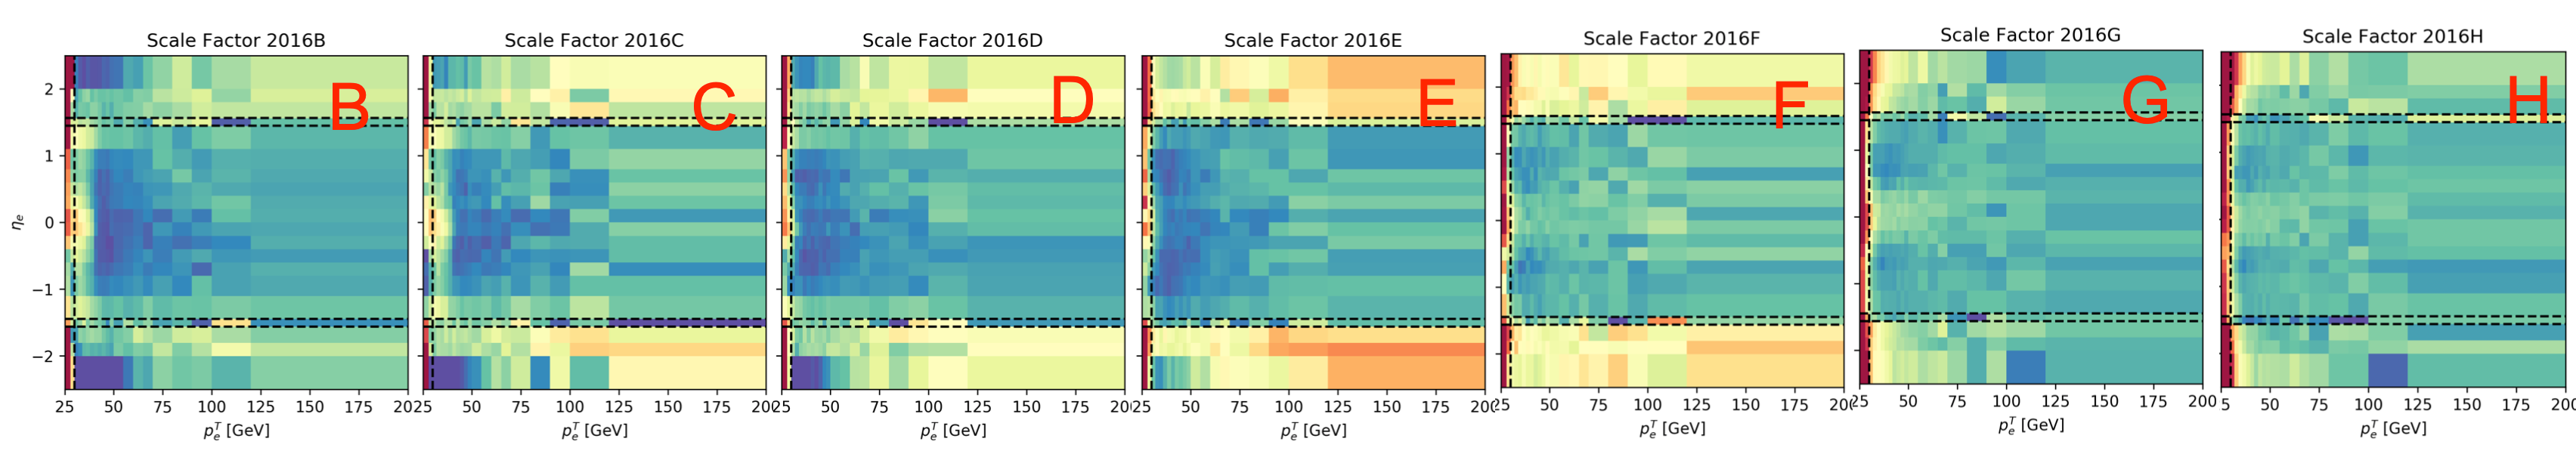
\includegraphics[width=0.99\textwidth]{chapters/Analysis/sectionCalibration/figures/eTrigger/result_period.png}
    \caption{Scale factors in each 2016 data taking period.}
    \label{fig:analysis:calibration:ele27SFperiods}
\end{figure}
% two shifts
The systematical uncertainties of the scale factors are estimated by ``two shifts" approach:
\begin{enumerate}
  \item shift up the \pt threshold for tagging electron by 10\GeV to simulate a different trigger. This estimates the systematical effect that some L1 seed could have a threshold of 32\GeV.
  \item shift up and down the probing electron \pt by 0.5\GeV. This estimates the effect of the electron energy scale.
\end{enumerate}
\noindent The systematical uncertainties are estimated by the "two shifts" are shown in Figure~\ref{fig:analysis:calibration:eTrSF_err_BCDEF} and \ref{fig:analysis:calibration:eTrSF_err_GH}.

\begin{figure}
    \centering
    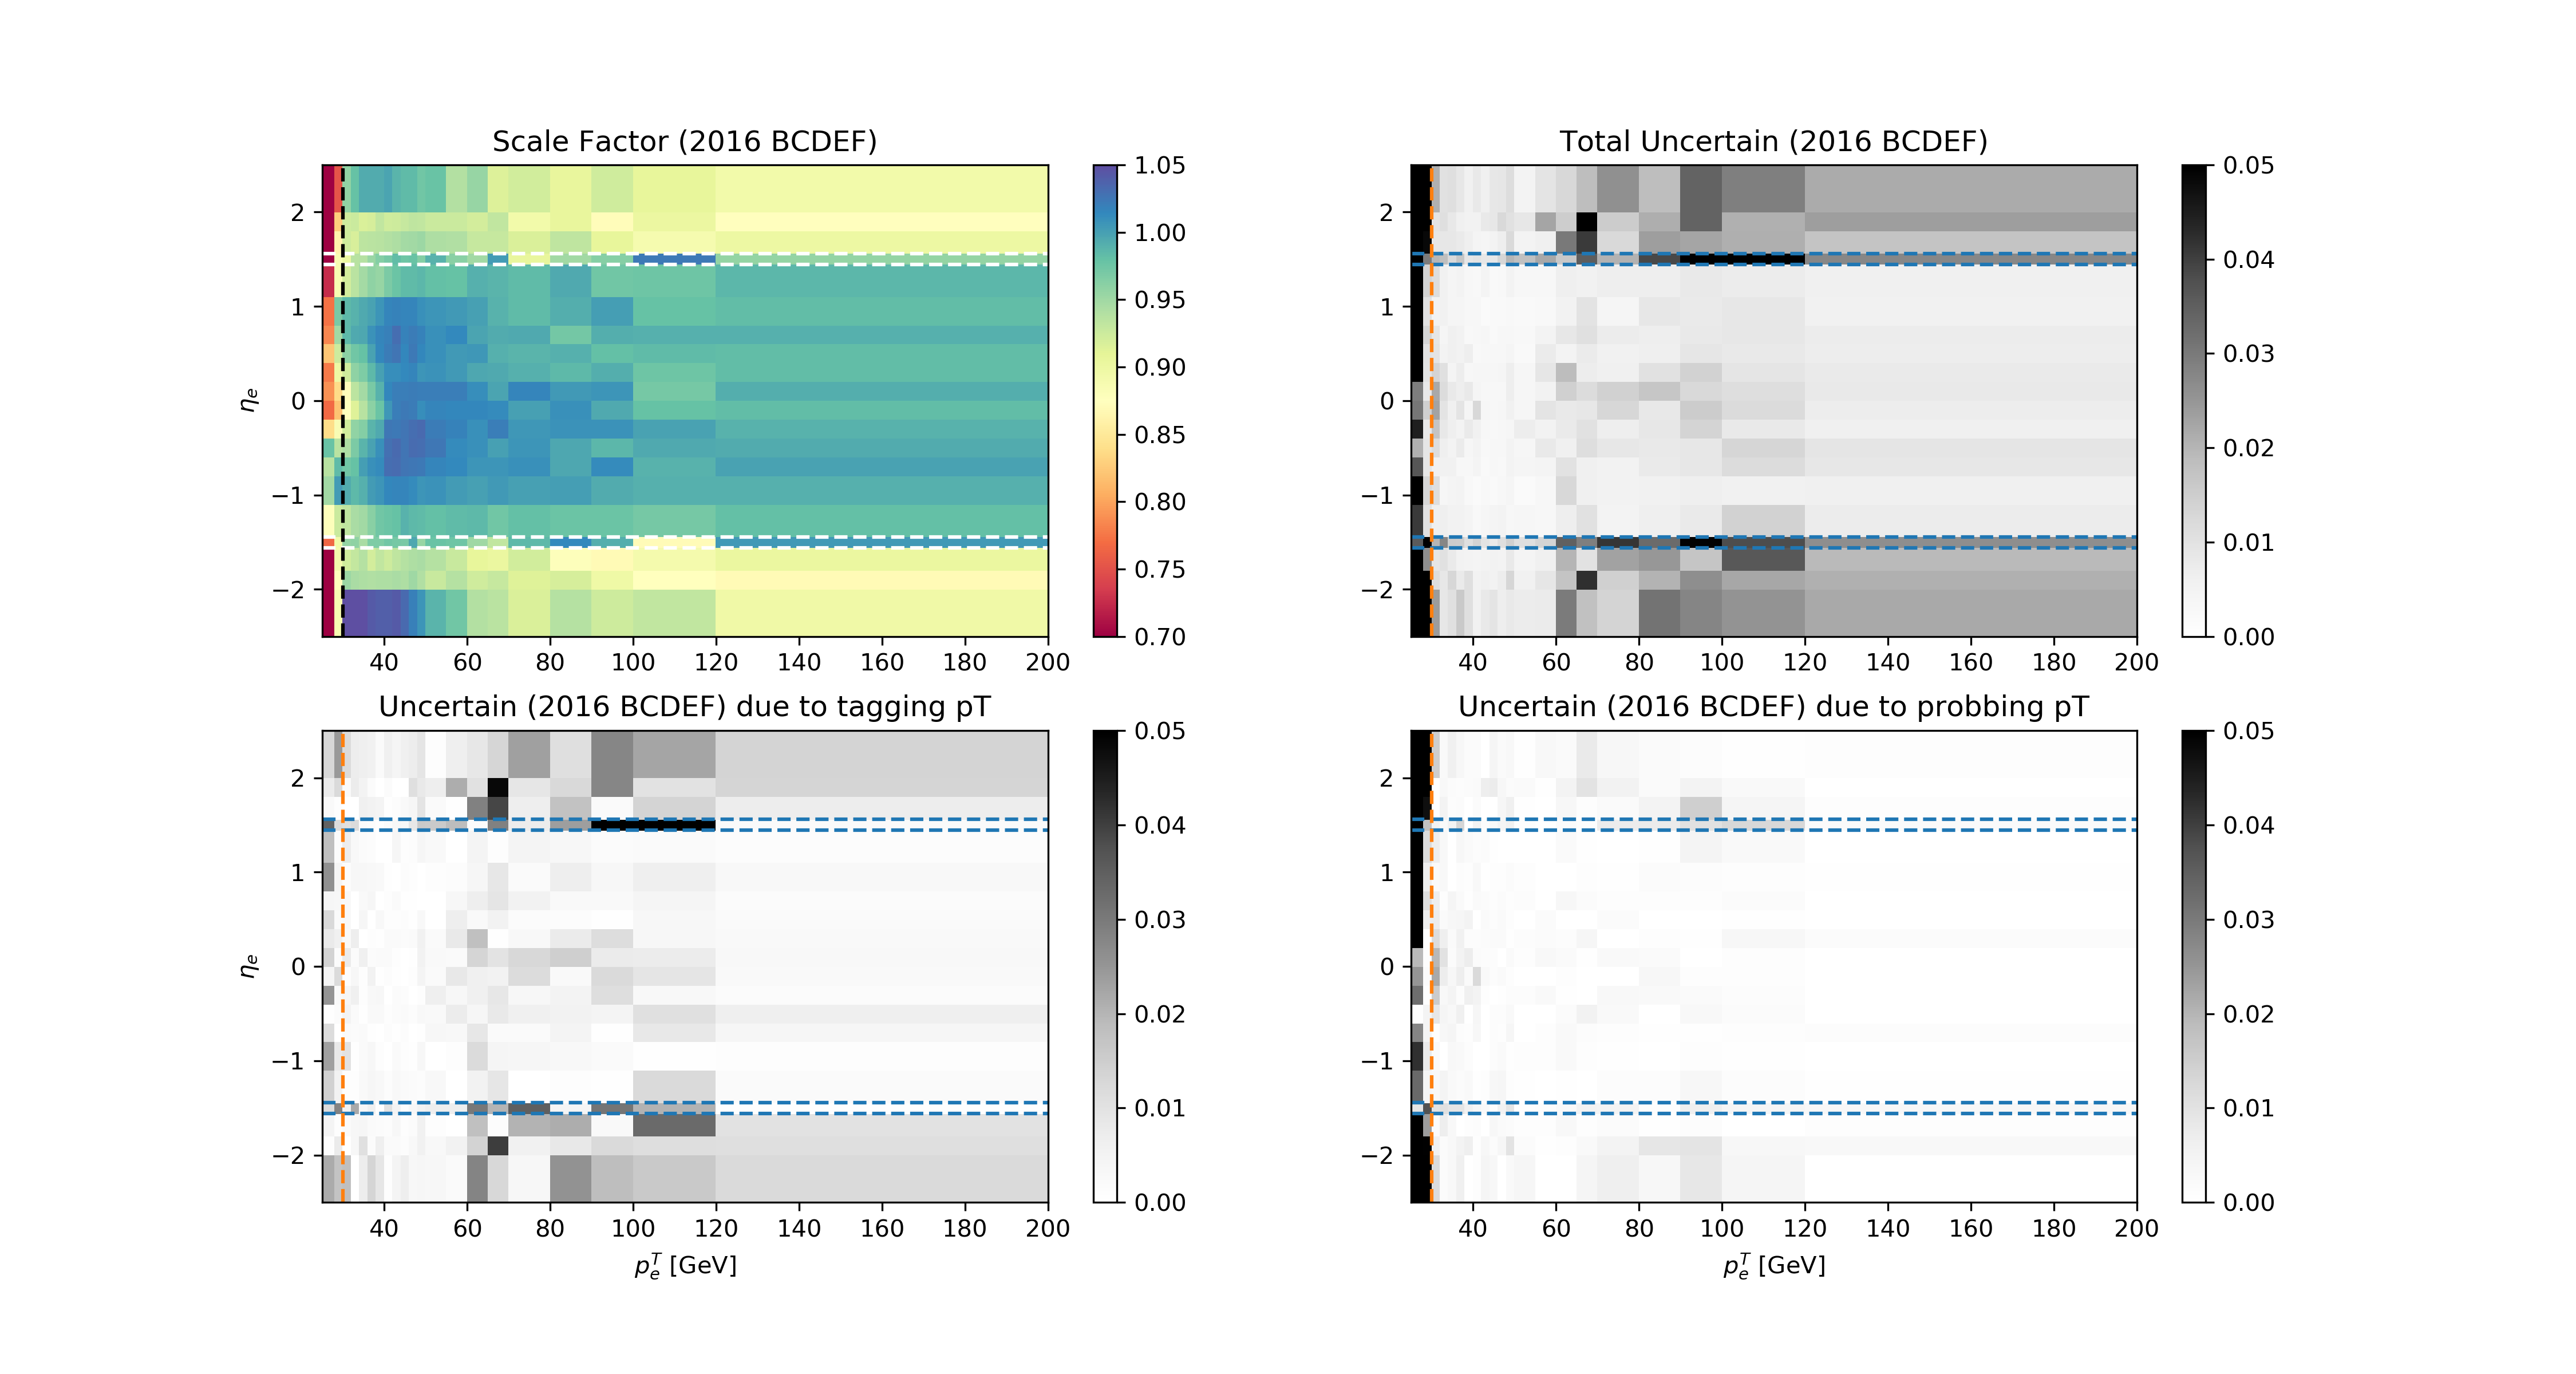
\includegraphics[width=0.99\textwidth]{chapters/Analysis/sectionCalibration/figures/eTrigger/result_BCDEF.png}
    \caption{Scale factors and uncertainties in the 2016 BCDEFF. Total uncertainties \emph{(upper right)} combines the ``two shifts" \emph{(lower)} and statistical uncertainties.}
    \label{fig:analysis:calibration:eTrSF_err_BCDEF}
\end{figure}

\begin{figure}
    \centering
    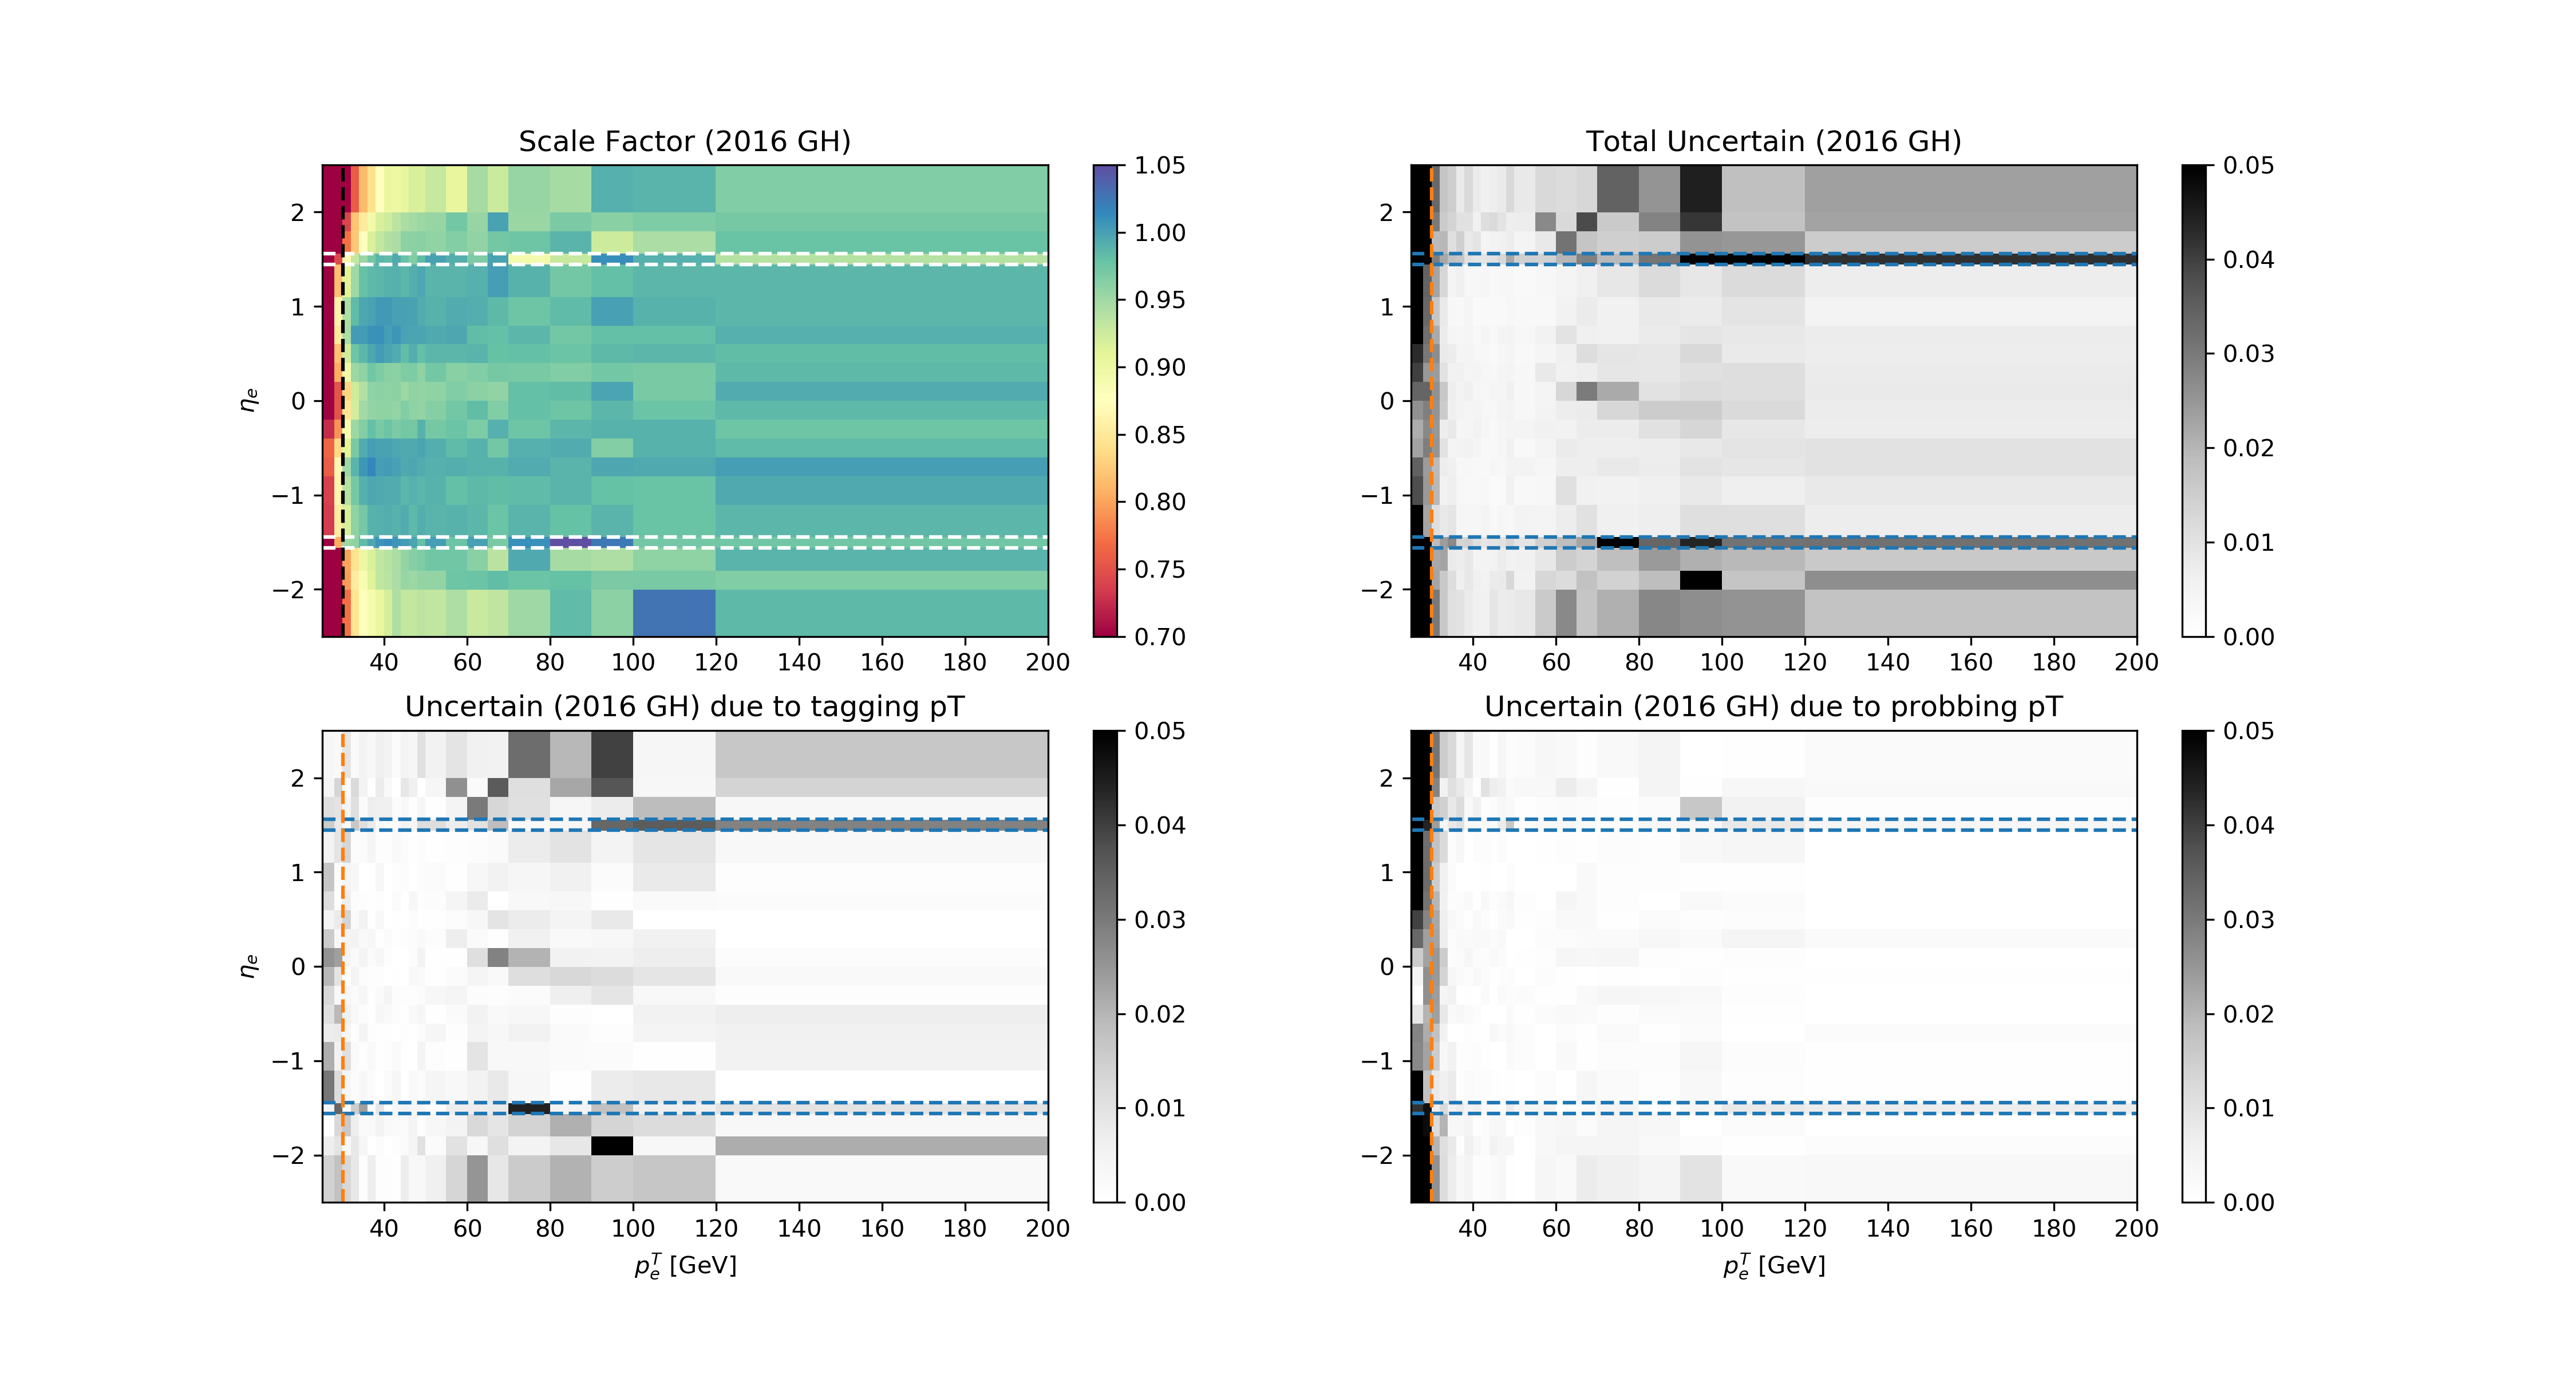
\includegraphics[width=0.99\textwidth]{chapters/Analysis/sectionCalibration/figures/eTrigger/result_GH.png}
    \caption{Scale factors and uncertainties in the 2016 GH. Total uncertainties \emph{(upper right)} combines the ``two shifts" \emph{(lower)} and statistical uncertainties.}
    \label{fig:analysis:calibration:eTrSF_err_GH}
\end{figure}


\subsubsection{Level-1 Trigger Prefiring in the Electromagnetic Calorimeter}
In 2016, the gradual timing shift of ECAL was not properly propagated to L1 trigger primitives (TP) resulting in a significant fraction of high eta TP being mistakenly associated to the previous bunch crossing. Since Level-1 rules forbid two consecutive bunch crossings to fire, an unpleasant consequence of this (in addition to not finding the TP in the correct bunch crossing) is that events can self-veto if a significant amount of ECAL energy is found in the region of $2.0<|\eta|<3.0$. This effect is not modeled by the simulations. Therefore scale factors are applied to reweight the events. The scale factors for ECAL prefiring corrections is defined as
\begin{equation*}
    SF = \prod_{i=\PGg,jet}\bigg(1-\epsilon_i(\pt, \eta) \bigg)
\end{equation*}
\noindent where $\epsilon_i(\pt, \eta)$ is the jet or photon prefiring probability and the corresponding 2D maps are provided by the EGamma POG, shown in Figure~\ref{fig:analysis:calibration:prefiring}. The prefiring $SF$ on average scales the simulated events down by about 1-2\%.
\begin{figure}[ht]
    \centering
    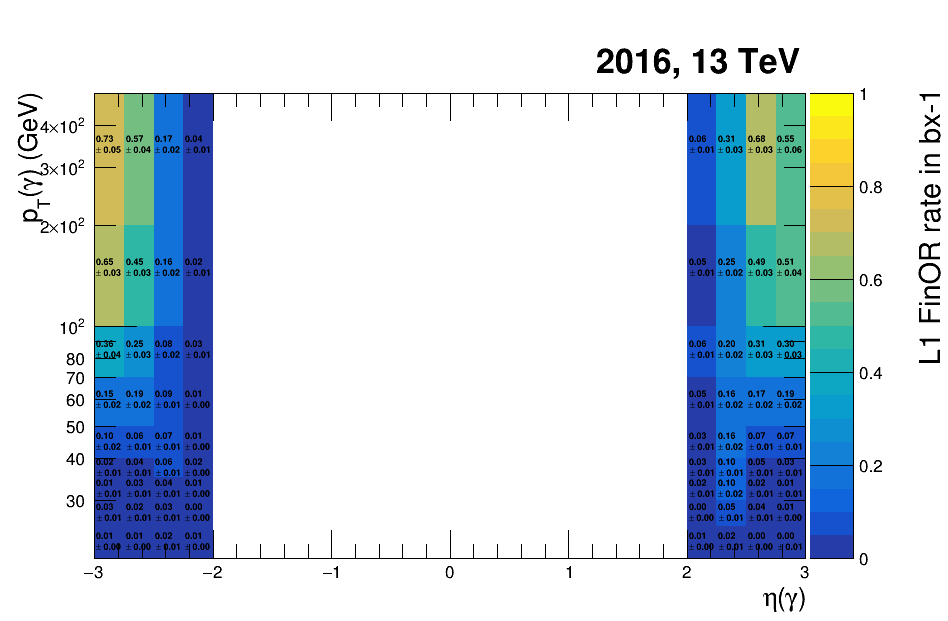
\includegraphics[width=0.49\textwidth]{chapters/Analysis/sectionCalibration/figures/prefiring/L1prefiring_photonpt_2016BtoH.png}
    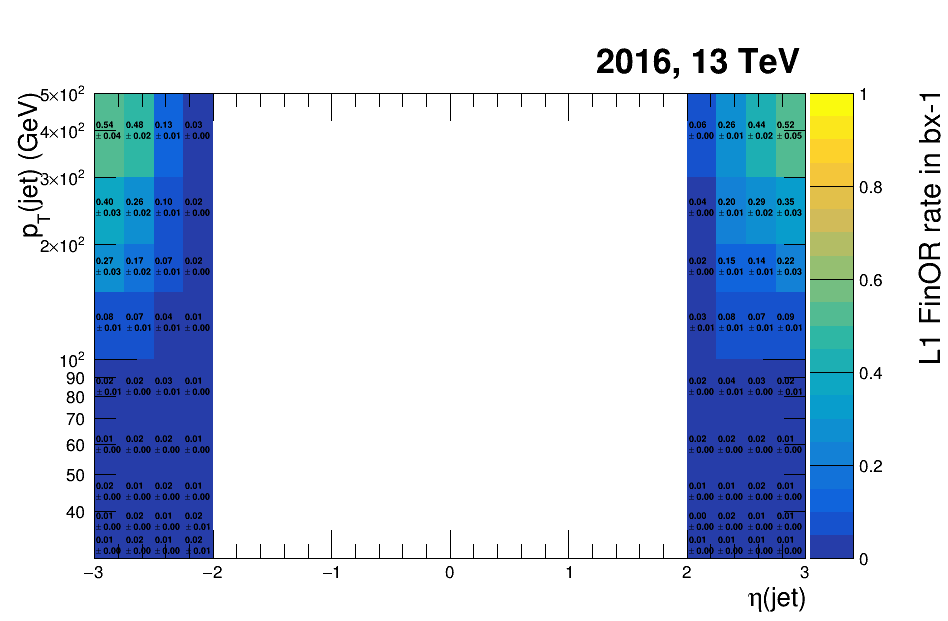
\includegraphics[width=0.49\textwidth]{chapters/Analysis/sectionCalibration/figures/prefiring/L1prefiring_jetpt_2016BtoH.png} 
    \caption{ Prefiring probabilities $\epsilon_i(\pt, \eta)$ for photons \emph{(left)} and jets \emph{(right)}. } 
    \label{fig:analysis:calibration:prefiring}
\end{figure}

\FloatBarrier








\subsection{Corrections for Jets Faking Hadronic Taus Misidentification Probability}
\label{sec:analysis:calibration:jetToTauh}

To account for difference of the $j\to\PGth$ faking probability in the data and simulation, scale factors are applied to simulated data based on the presence of $j\to\PGth$ in the events. While the scale factors of \PGth identification is provided by the POG, the scale factors for the misidentification have to be measured by each analysis due to the potential different jet environments in different analysis. Here we present a measurement of $SF_{j\to\PGth}$ using two side-band regions enriched with $j\to\PGth$. The $SF_{j\to\PGth}$ measurement is \pt and jet-favour dependent. Tight and VTight \PGth identification working points are considered. The two side-band regions are
\begin{itemize}
    \item \ttbar with $j\to\PGth$ region: selected with $\cem+\PGth$ final state. The selection requires exactly one muon and one electron with tight identification and isolation, plus one hadronic tau passing Tight or VTight working point. Corrections to reconstruction and selection of electron and muon are applied. The events has to fire either single muon trigger or single electron trigger.  The \pt threshold for triggering muon (electron) is 25 (30) \GeV, while for non-triggering muon (electron) is 10 (20) \GeV.  This selects a sample enriched with \ttbar with $\PQb \to \PGth$. 
    \item \zjets with $j\to\PGth$ region: $\cmm+\PGth$ and $\cee+\PGth$  final state are selected.  The selection requires exactly two muons or two electrons with tight identification and isolation, plus one hadronic tau passing Tight or VTight working point.  Corrections to reconstruction and selection of electron and muon are applied. The trigger and \pt thresholds of leptons are the same as $\cem+\PGth$ final state.  This selects a sample enriched with \zjets with a light jet misidentified as \PGth. 
\end{itemize}
\noindent Note that the $\cem+\PGth$, $\cmm+\PGth$, $\cee+\PGth$ channels are developed based on the $\cem$, $\cmm$, $\cee$ channels in the \BWl measurement, using the same dilepton selection but replacing jet and \PQb tag requirements with one additional Tight or VTight \PGth. The kinematics distribution of $\cem+\PGth$, $\cmm+\PGth$, $\cee+\PGth$ channels are shown in Figure~\ref{fig:analysis:calibration:llt_tight} and \ref{fig:analysis:calibration:llt_vtight} for Tight and VTight working point, respectively. 


The origins of selected \PGth are tagged based on generator-level truth. For each selected \PGth, if there is a gen-level \PGth found within $\DR = 0.3$, the \PGth is tagged as true identification.  If not a true identification, we try to match it with jet in the vetoed-jet collection and tag it as $j \to \PGth$, flavor of which equals to the gen-level flavor of the jet correspondence.  In the rare cases where multiple jet correspondences are found, the one with highest \pt is considered.  Also in rare cases where neither gen-level \PGth match nor jet correspondence are found, the \PGth is tagged as null. The origins of \PGth is also included on the right column in Figure~\ref{fig:analysis:calibration:llt_tight} and \ref{fig:analysis:calibration:llt_vtight}.
\begin{figure}
    \centering
    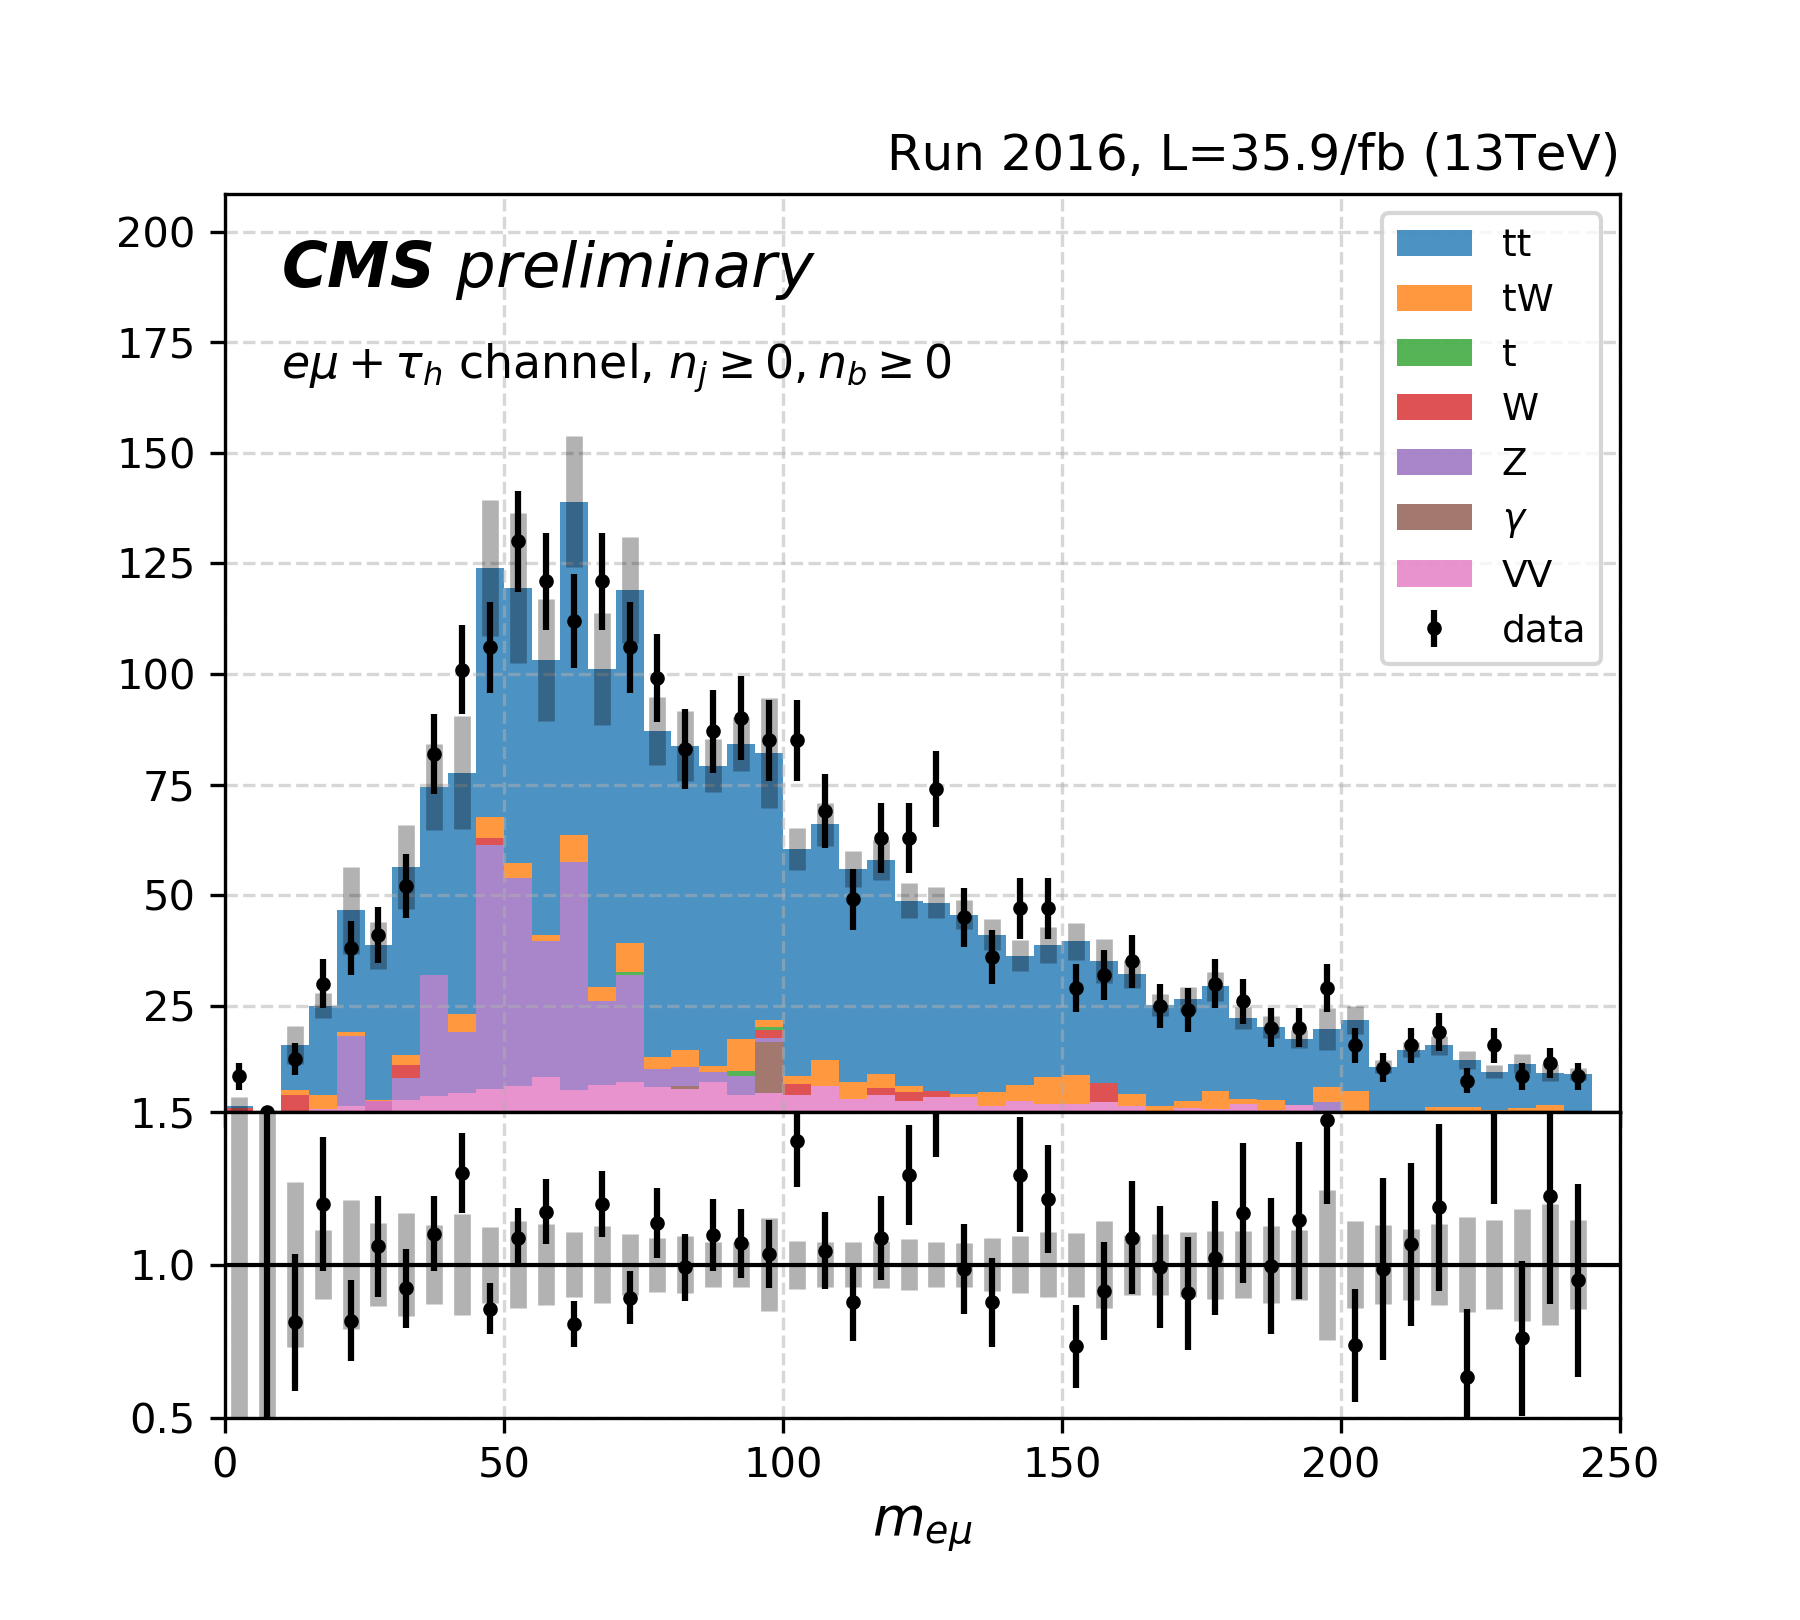
\includegraphics[width=0.32\textwidth]{chapters/Analysis/sectionCalibration/figures/jetToTauh/emutau_dilepton_mass_pickles_lltauTight.png}
    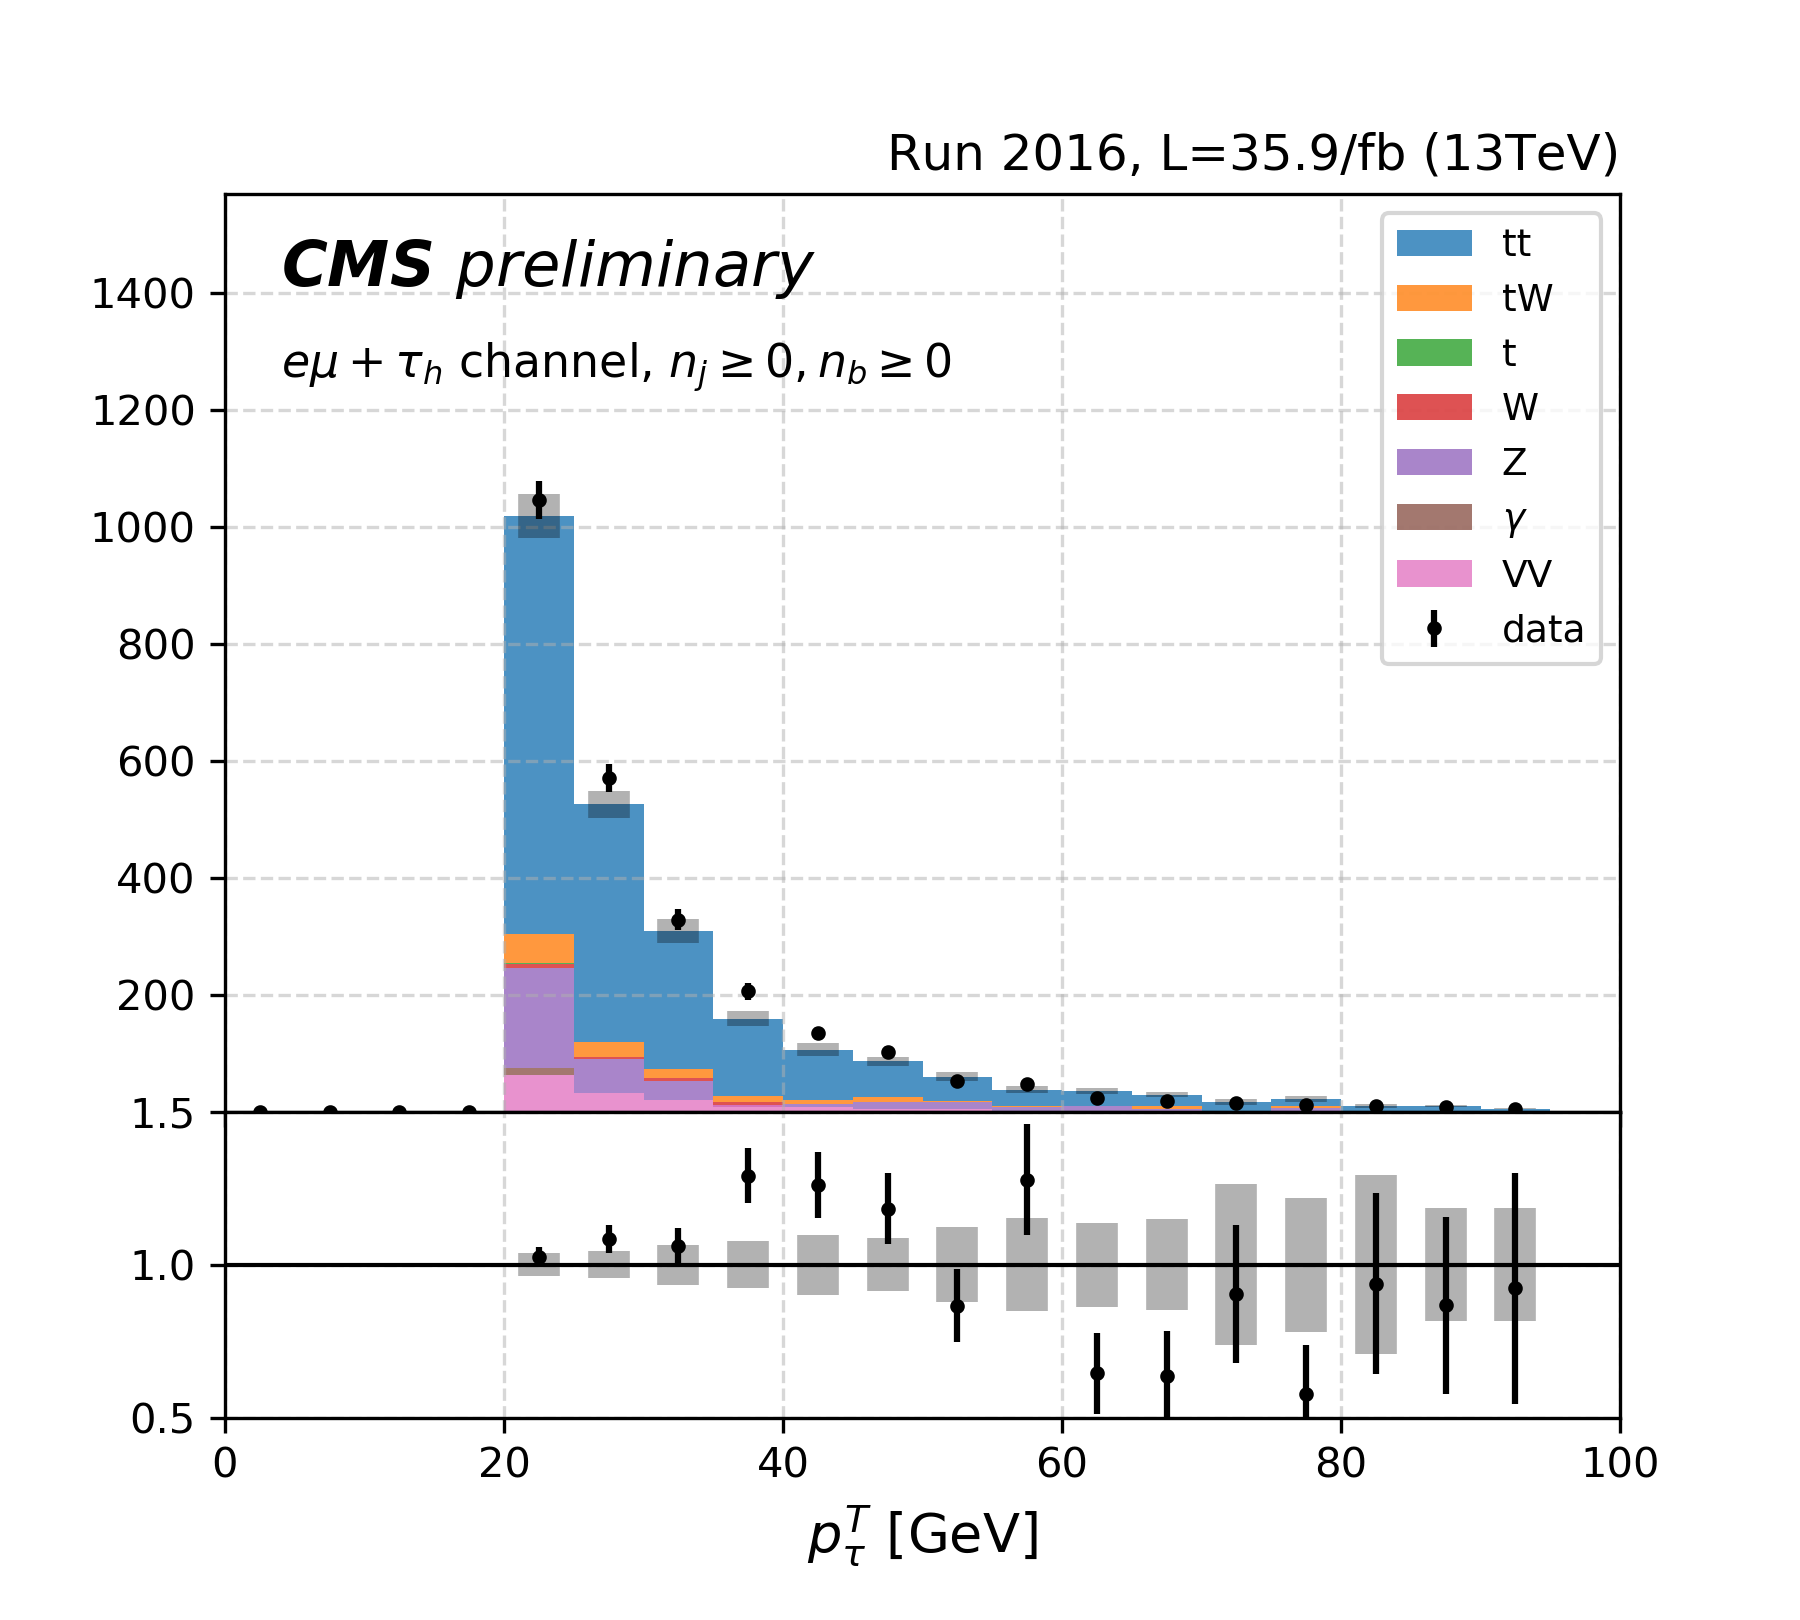
\includegraphics[width=0.32\textwidth]{chapters/Analysis/sectionCalibration/figures/jetToTauh/emutau_tauPt_pickles_lltauTight.png}
    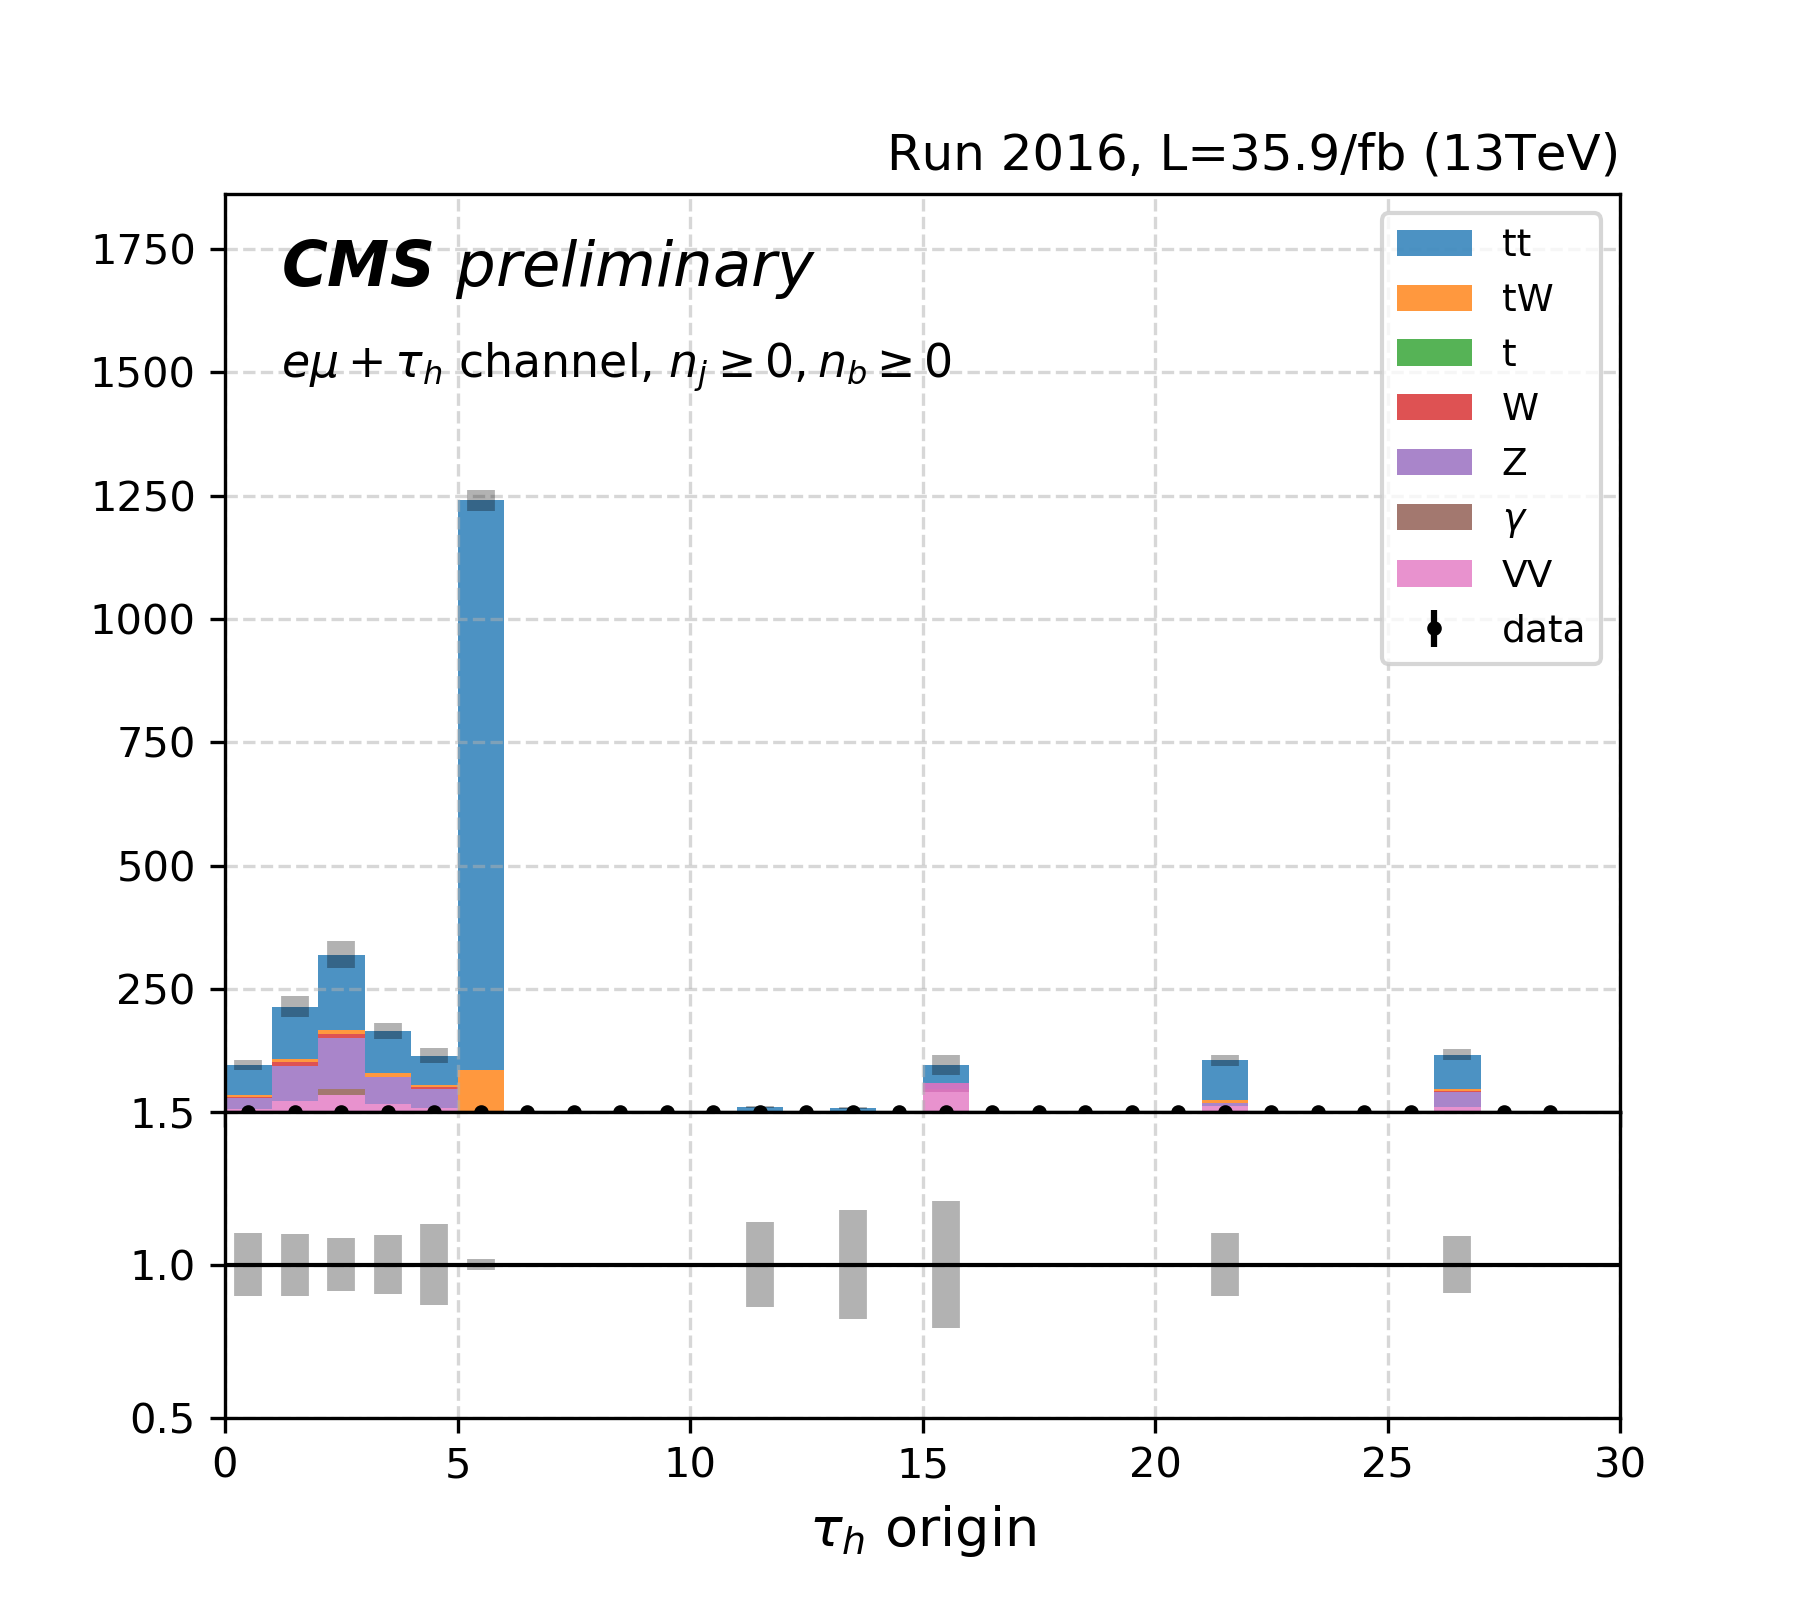
\includegraphics[width=0.32\textwidth]{chapters/Analysis/sectionCalibration/figures/jetToTauh/emutau_tauGenFlavor_pickles_lltauTight.png}
    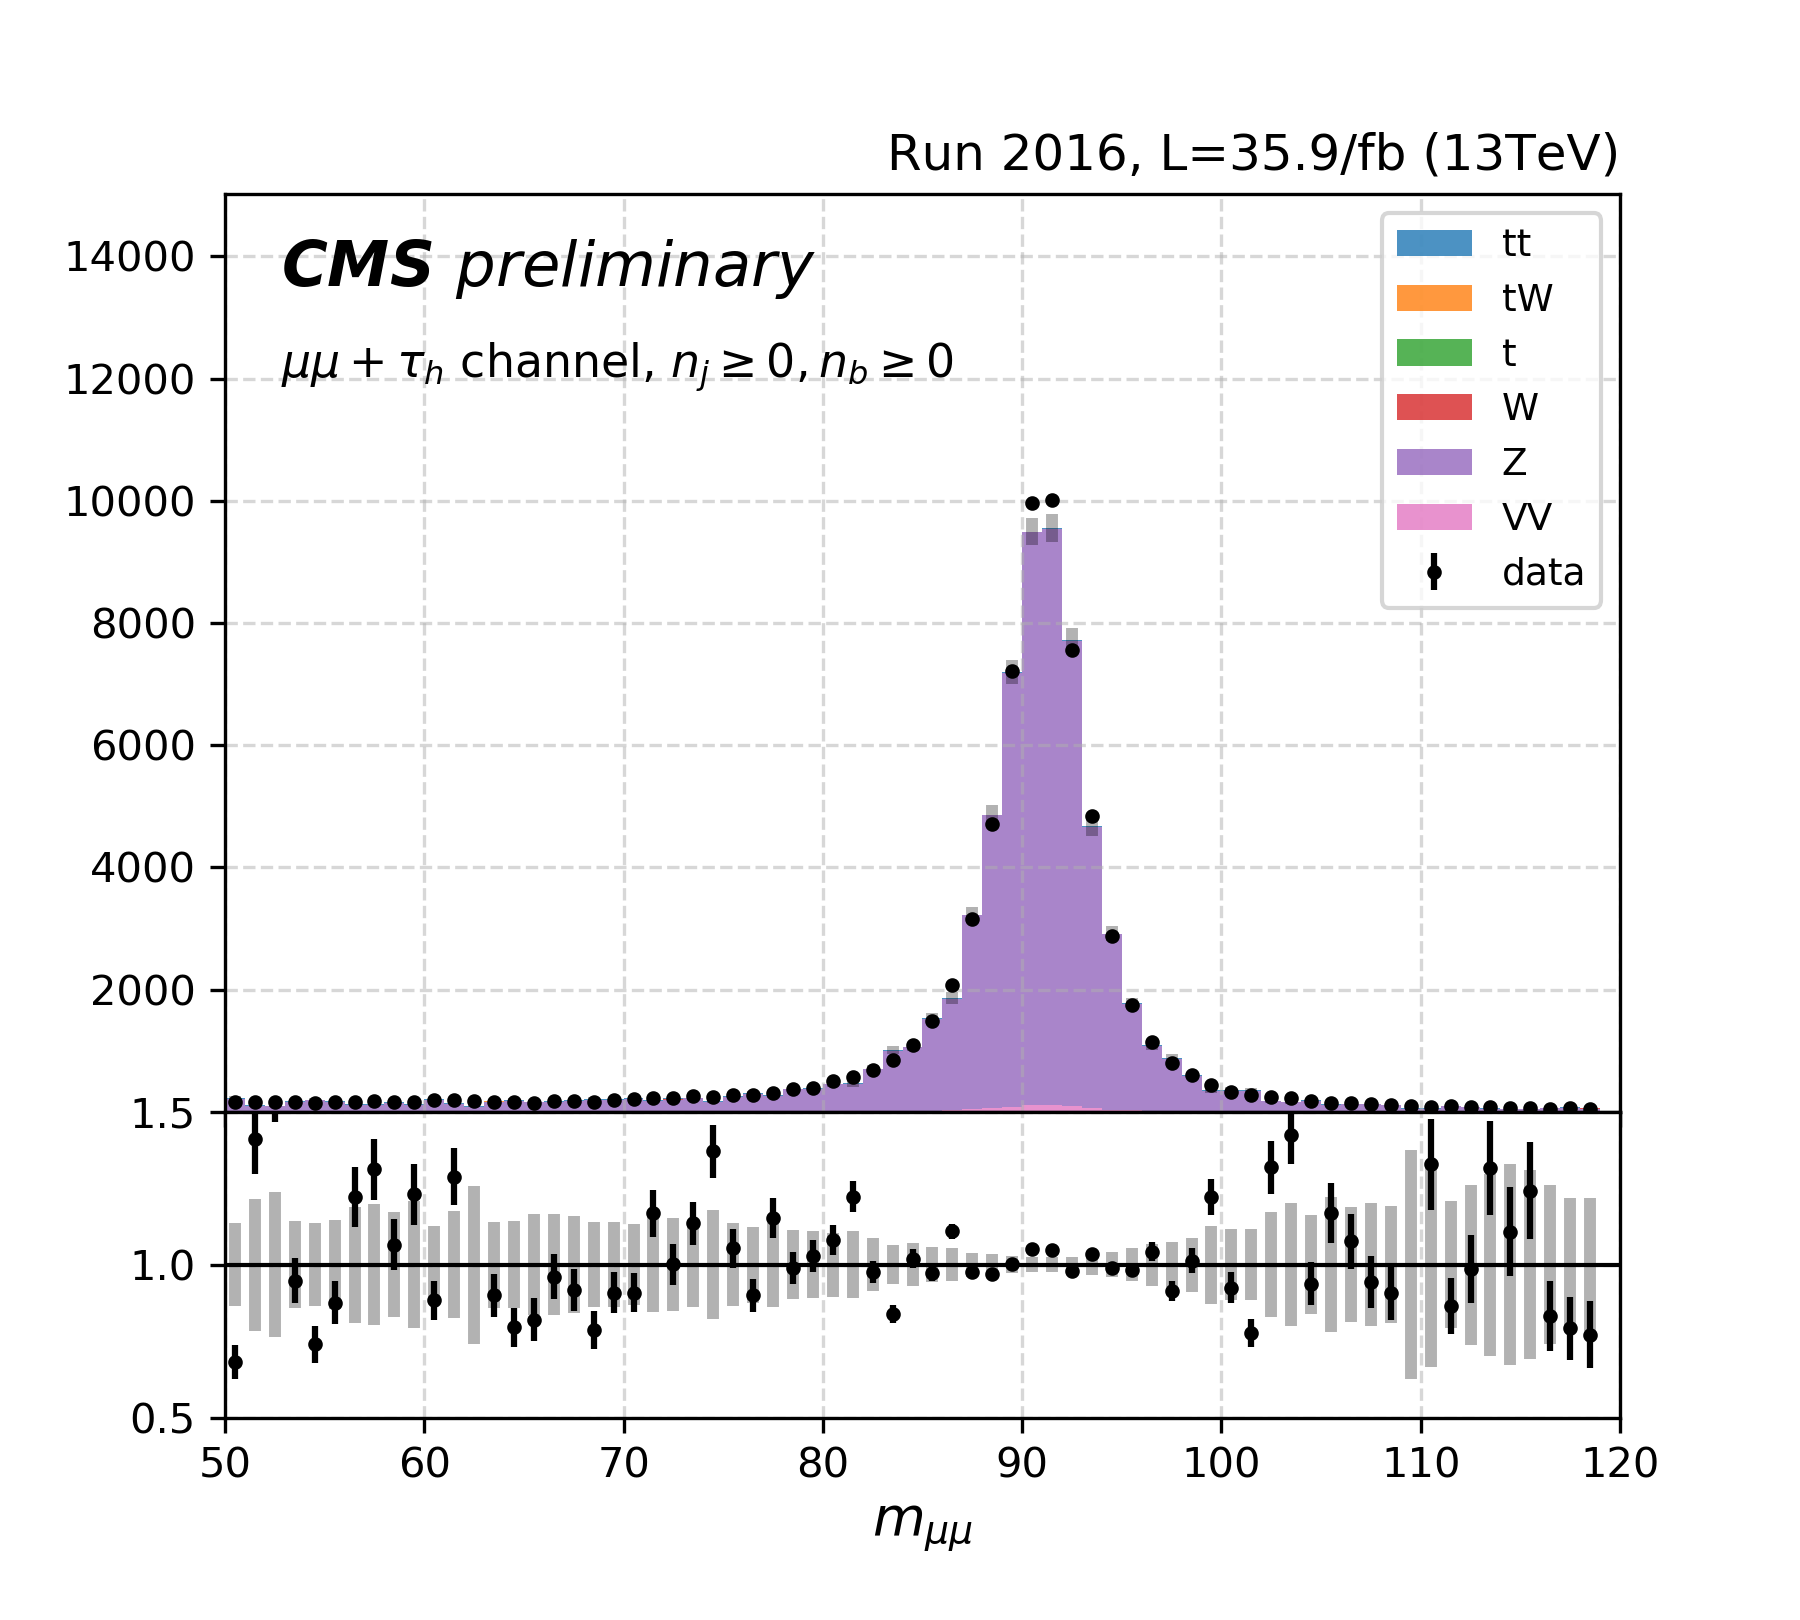
\includegraphics[width=0.32\textwidth]{chapters/Analysis/sectionCalibration/figures/jetToTauh/mumutau_dilepton_mass_pickles_lltauTight.png}
    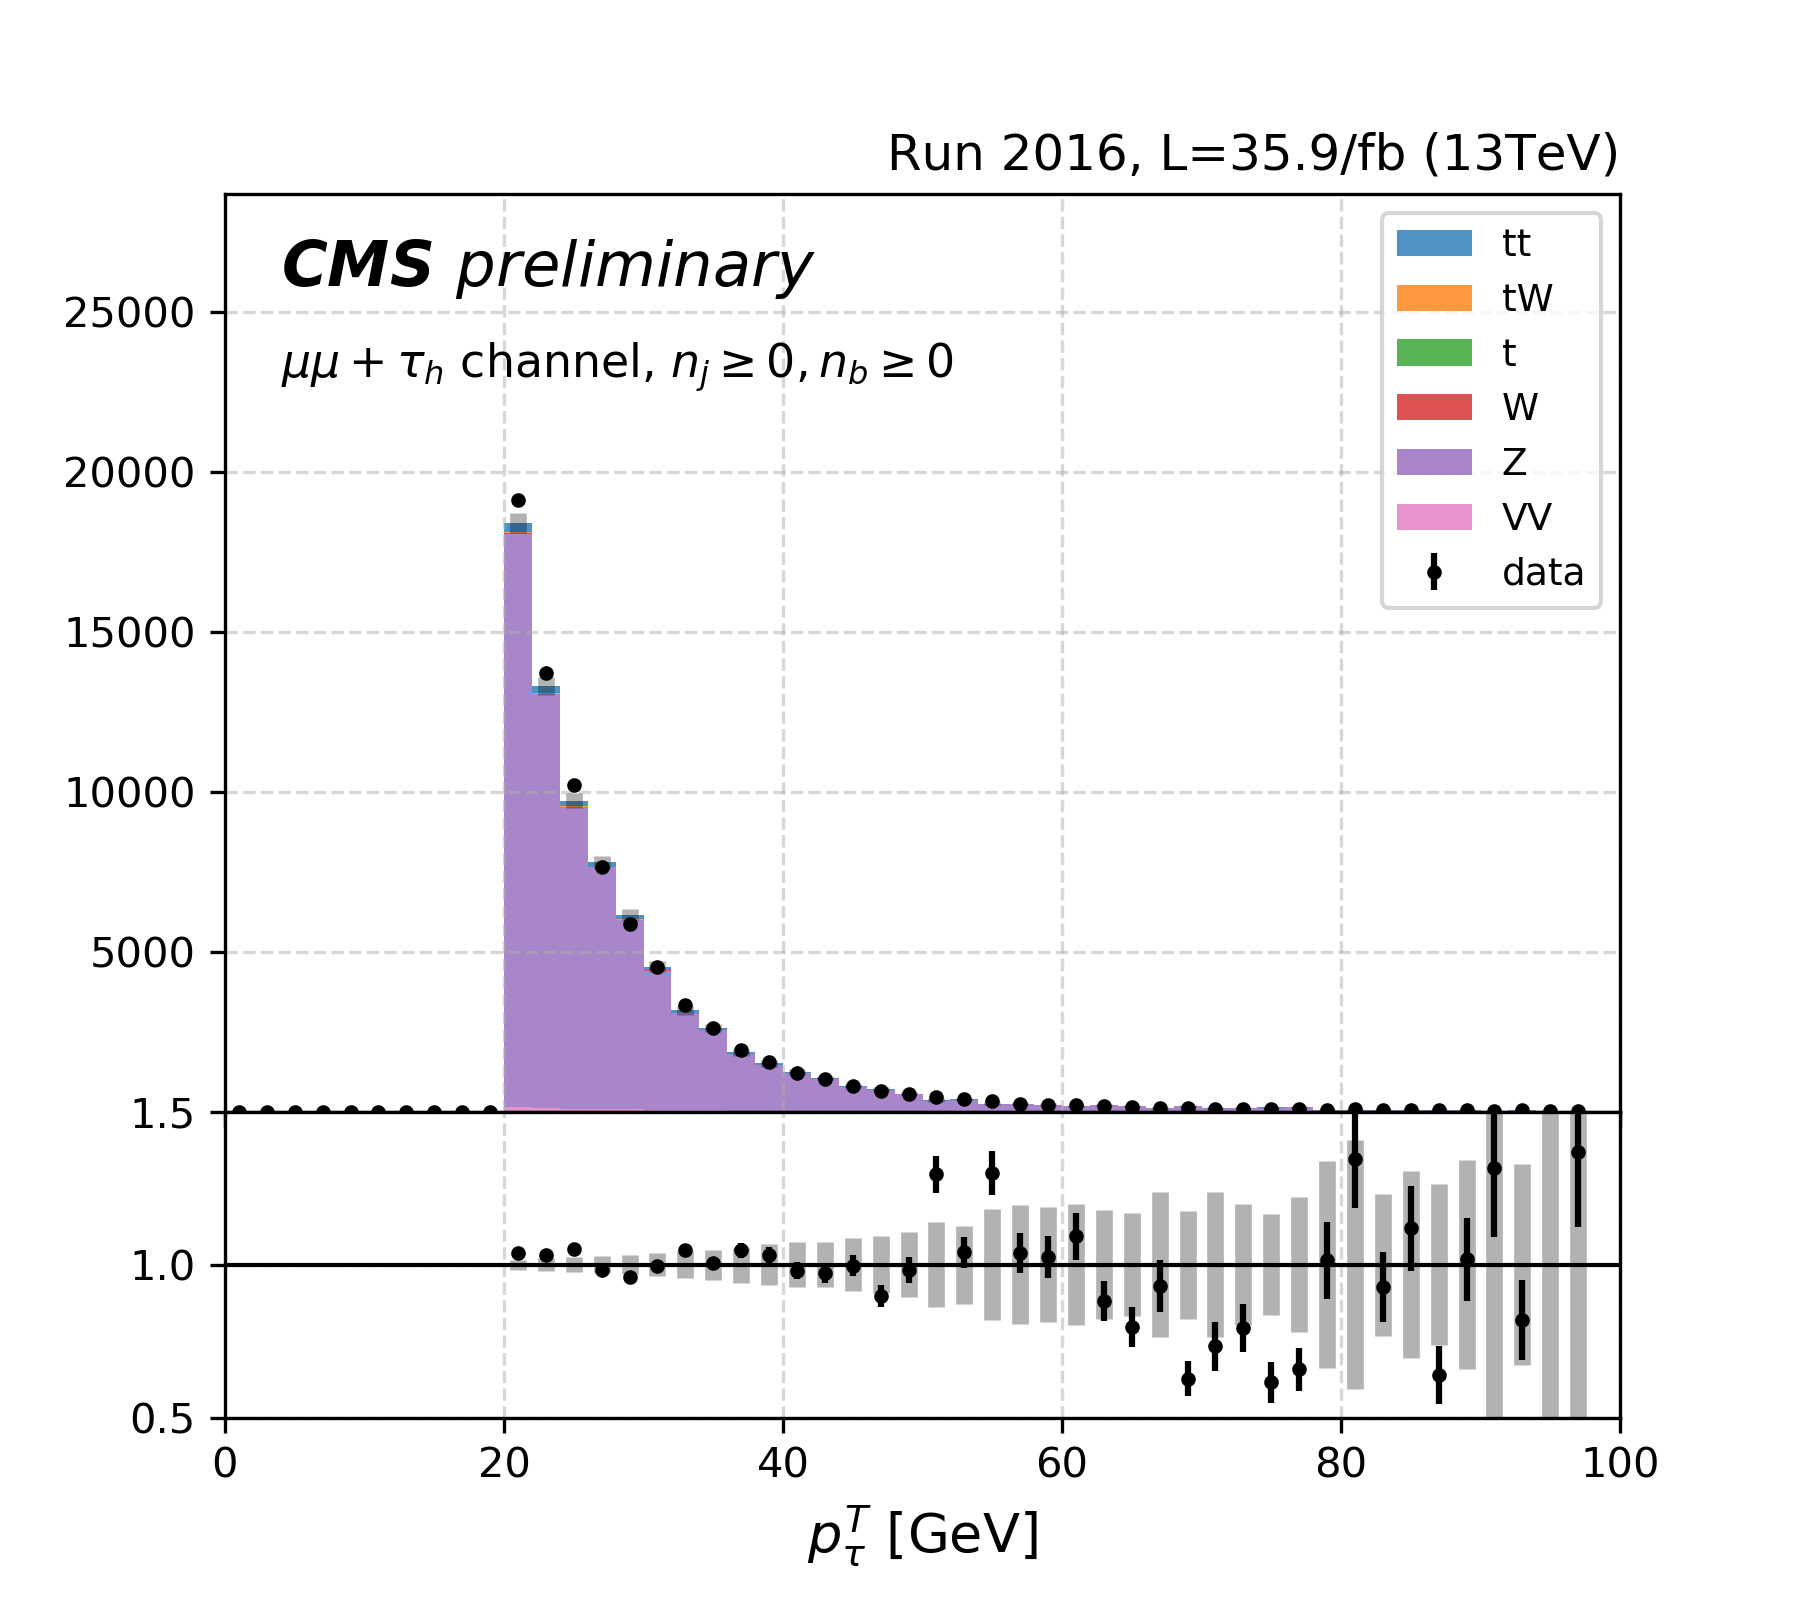
\includegraphics[width=0.32\textwidth]{chapters/Analysis/sectionCalibration/figures/jetToTauh/mumutau_tauPt_pickles_lltauTight.png}
    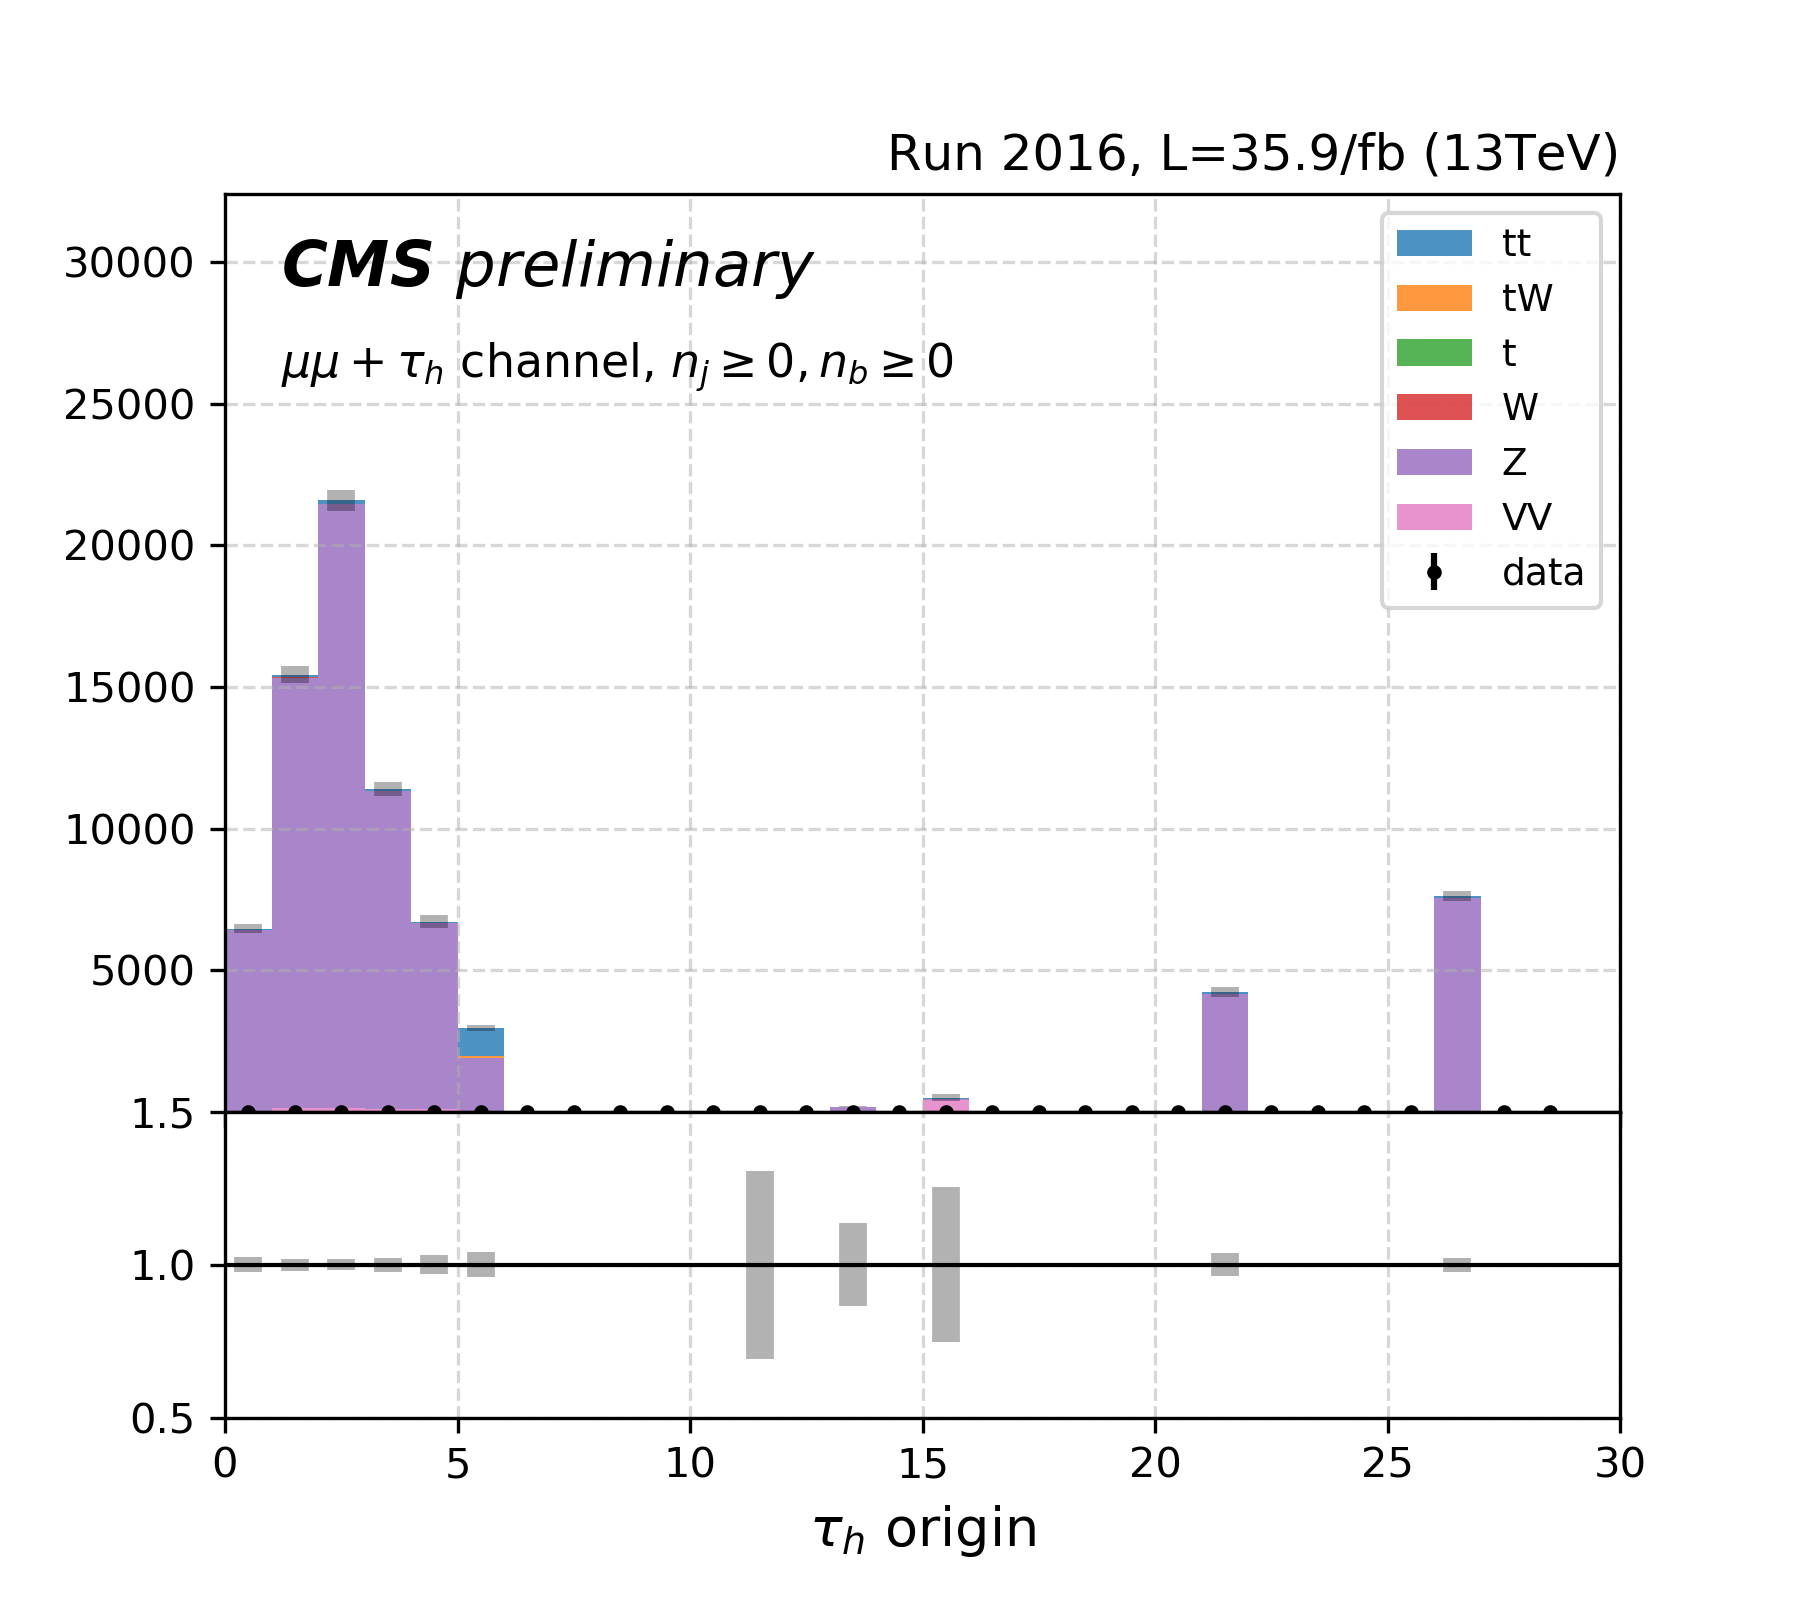
\includegraphics[width=0.32\textwidth]{chapters/Analysis/sectionCalibration/figures/jetToTauh/mumutau_tauGenFlavor_pickles_lltauTight.png}
    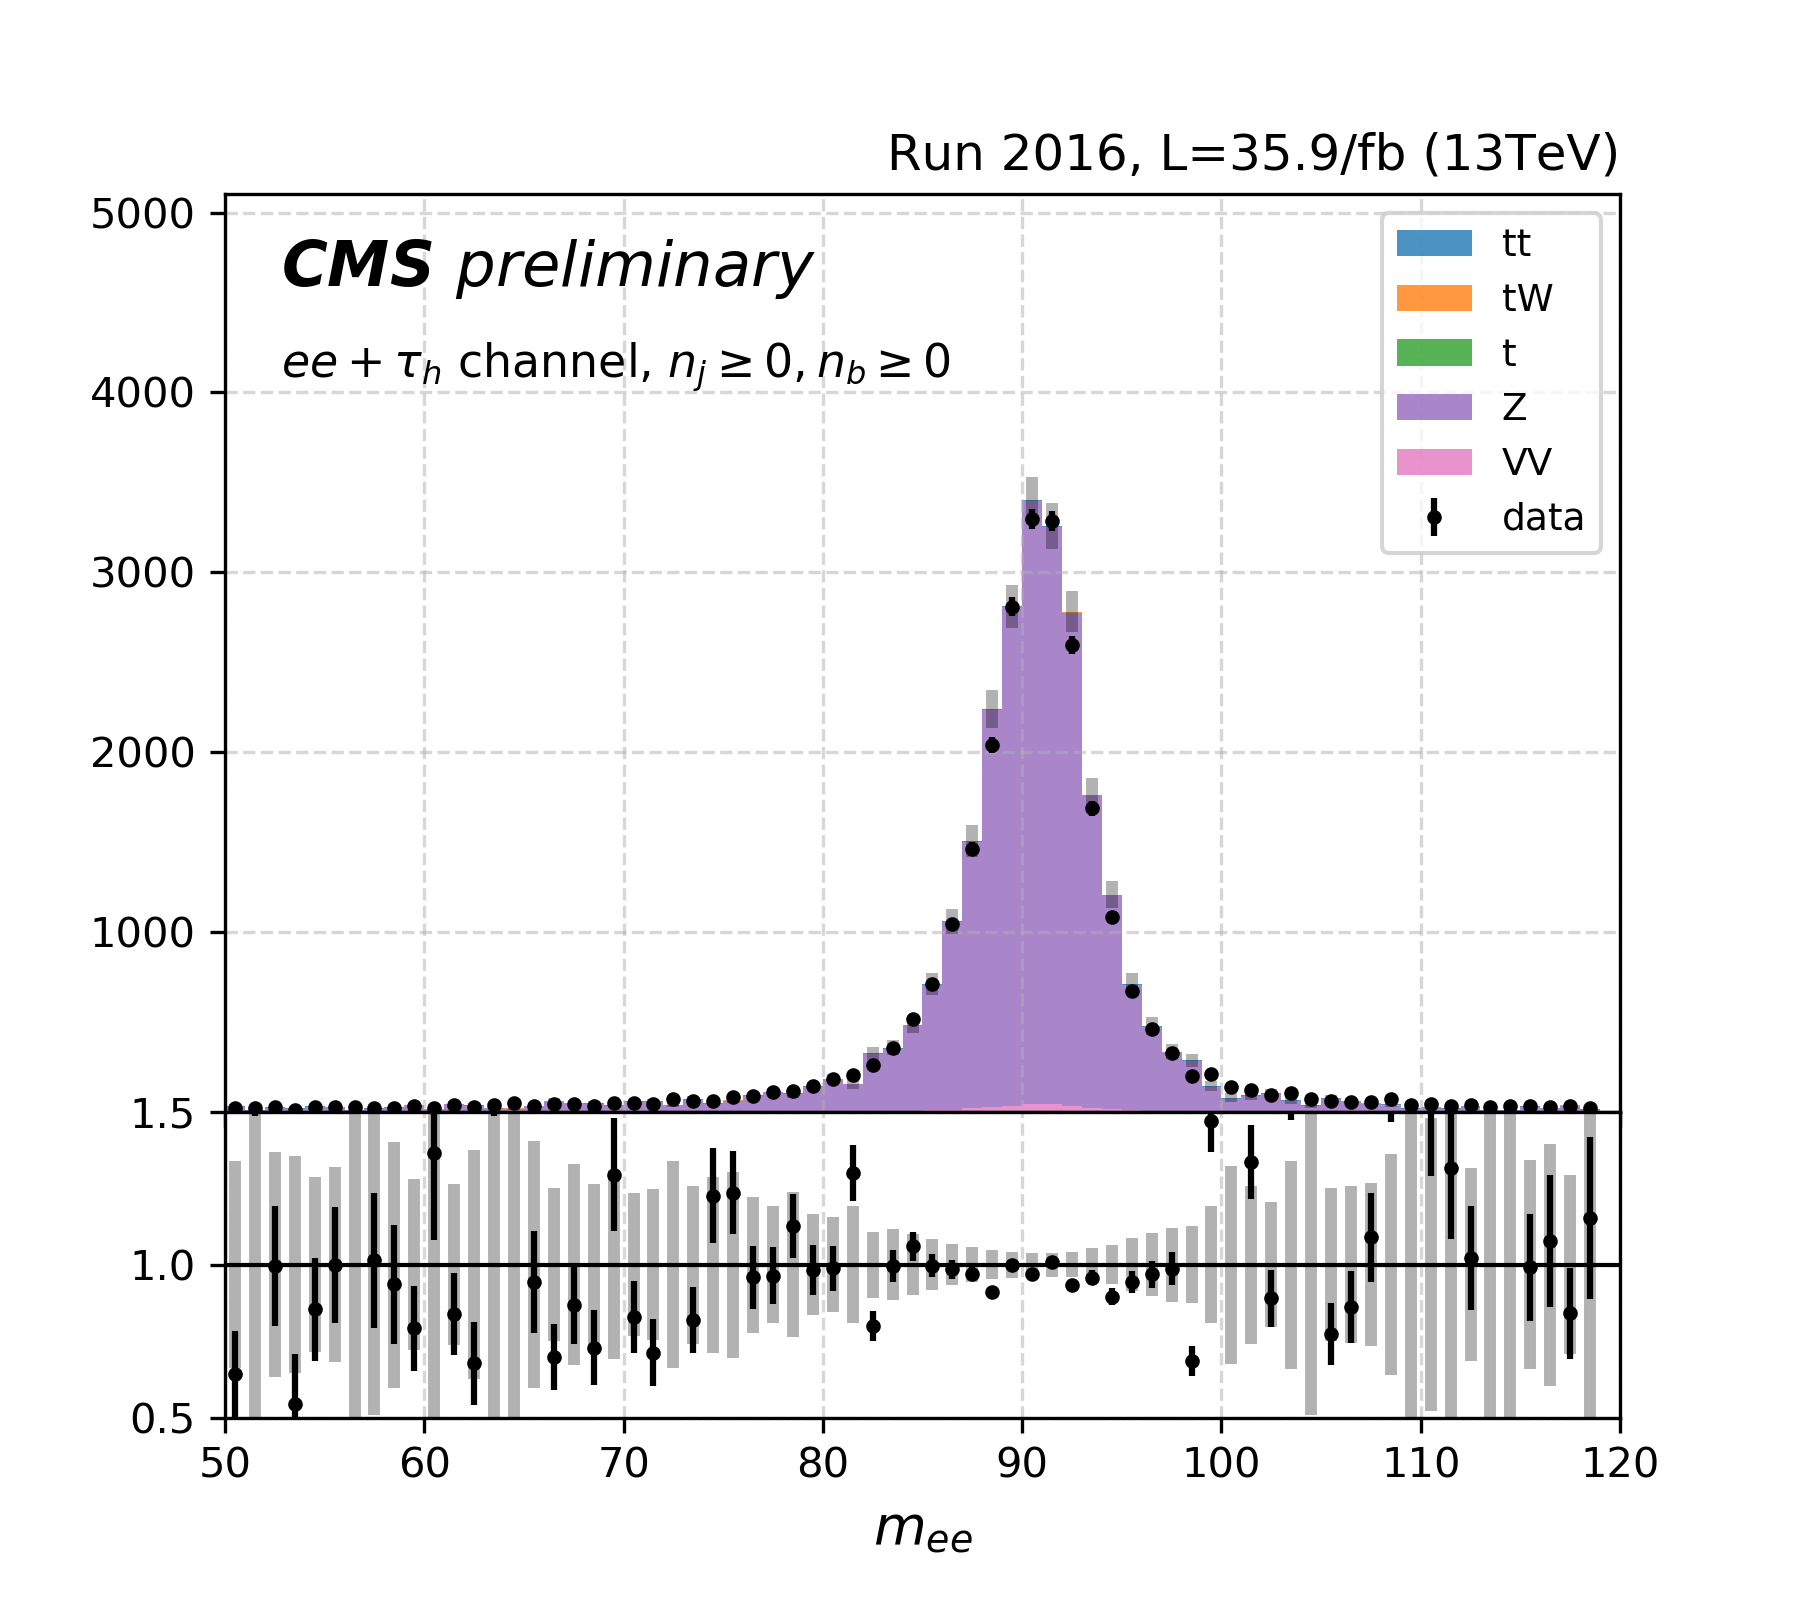
\includegraphics[width=0.32\textwidth]{chapters/Analysis/sectionCalibration/figures/jetToTauh/eetau_dilepton_mass_pickles_lltauTight.png}
    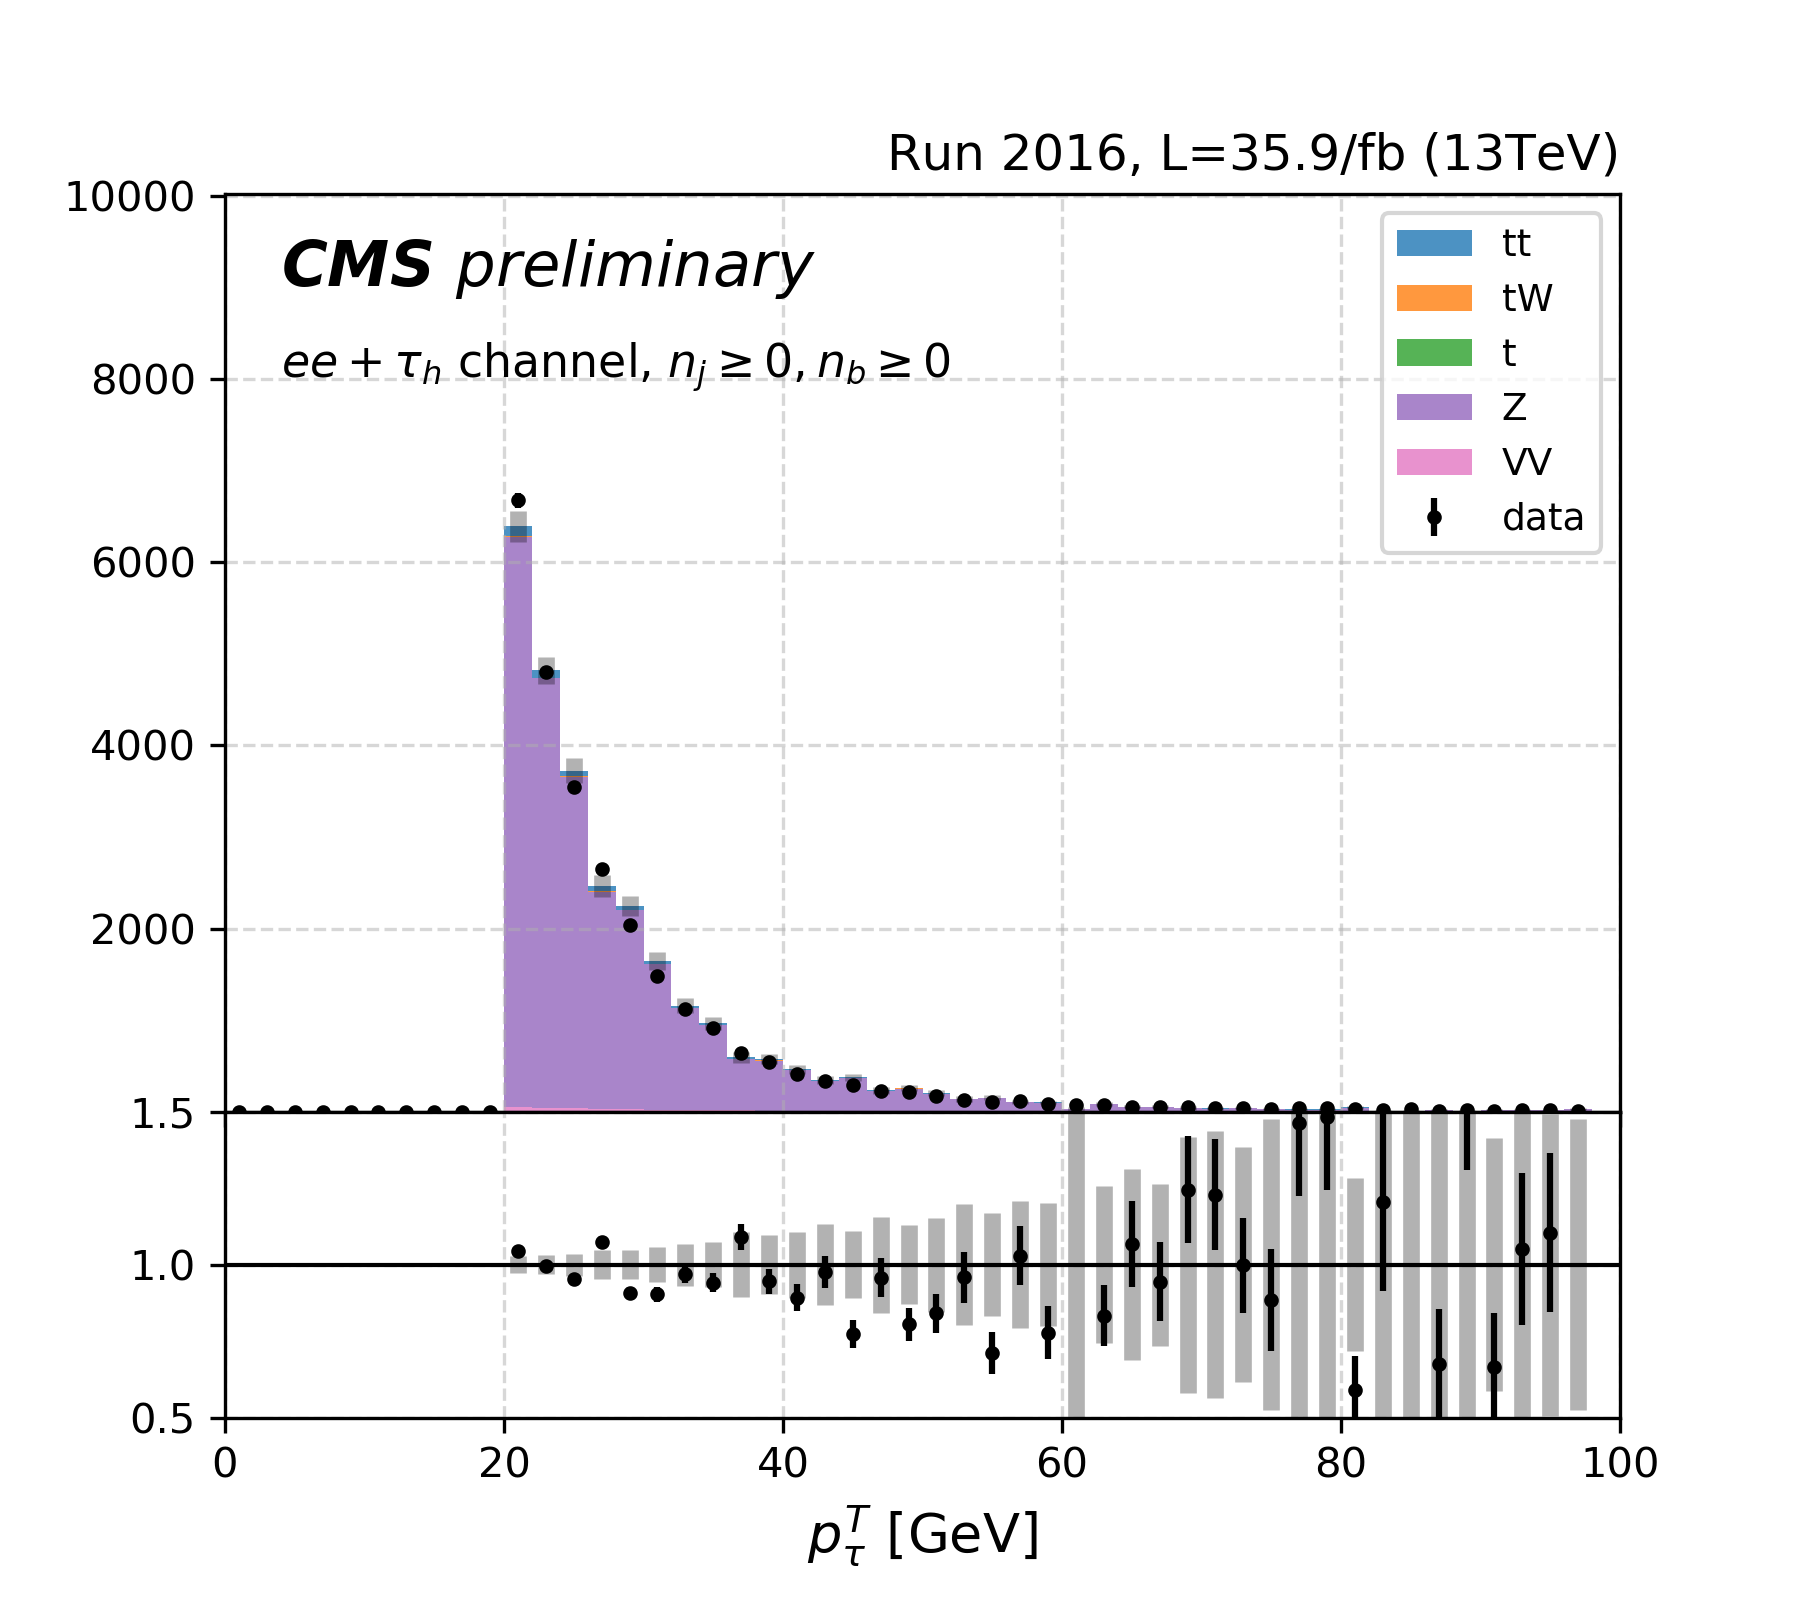
\includegraphics[width=0.32\textwidth]{chapters/Analysis/sectionCalibration/figures/jetToTauh/eetau_tauPt_pickles_lltauTight.png}
    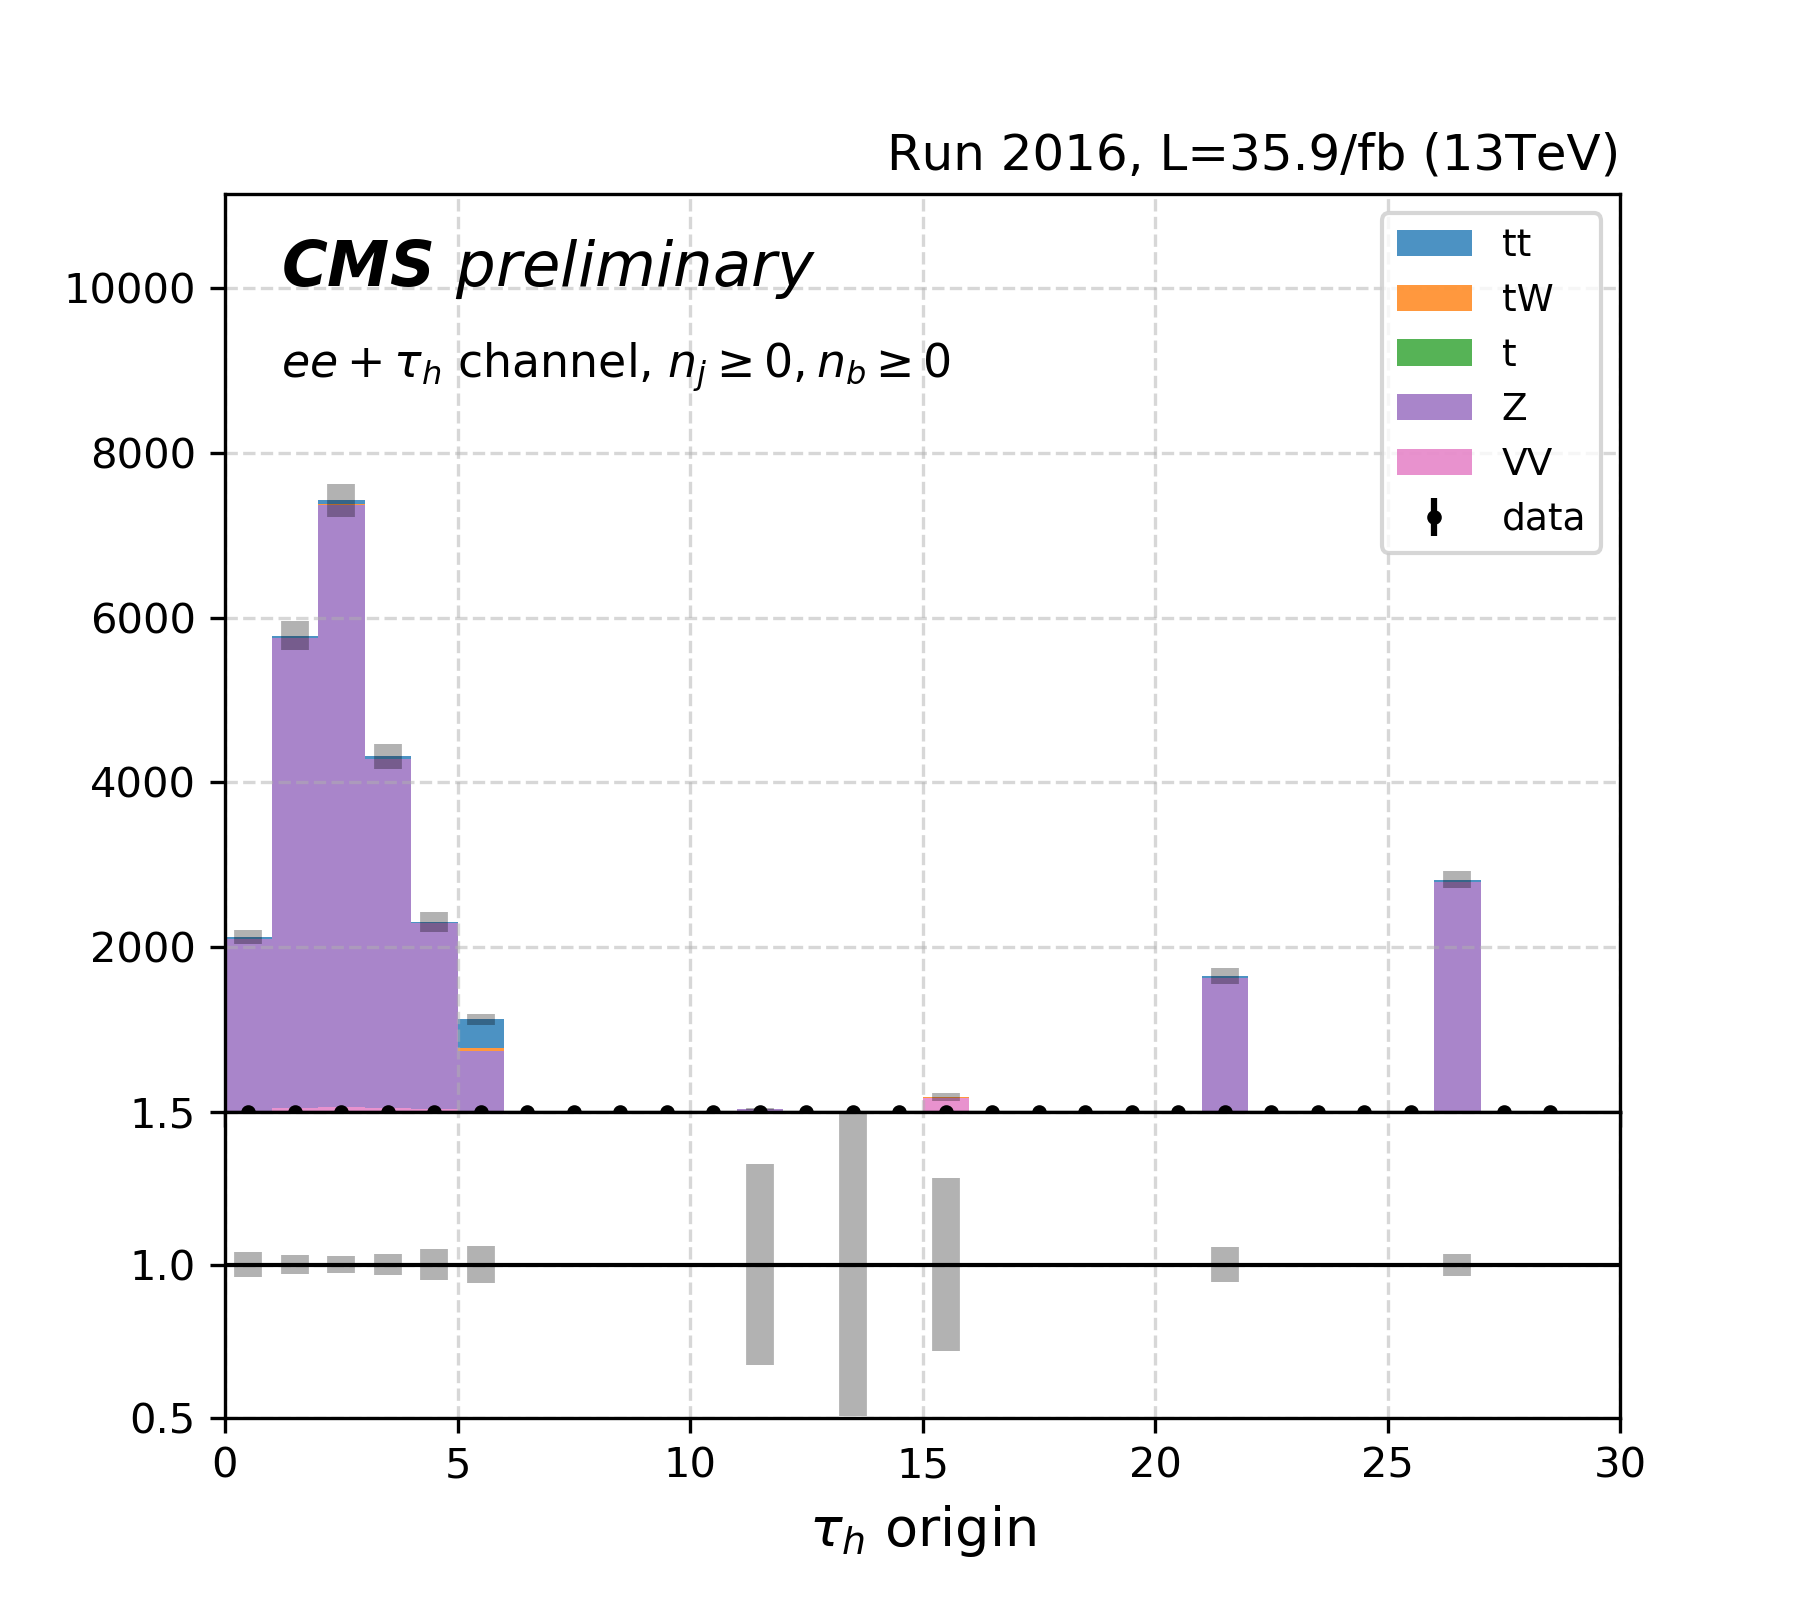
\includegraphics[width=0.32\textwidth]{chapters/Analysis/sectionCalibration/figures/jetToTauh/eetau_tauGenFlavor_pickles_lltauTight.png}
    \caption{The kinematics distribution of $\cem+\PGth$, $\cmm+\PGth$, $\cee+\PGth$ channels with Tight \PGth working point.}
    \label{fig:analysis:calibration:llt_tight}
\end{figure}
\begin{figure}
    \centering
    \includegraphics[width=0.32\textwidth]{chapters/Analysis/sectionCalibration/figures/jetToTauh/emutau_dilepton_mass_pickles_lltauvTight.png}
    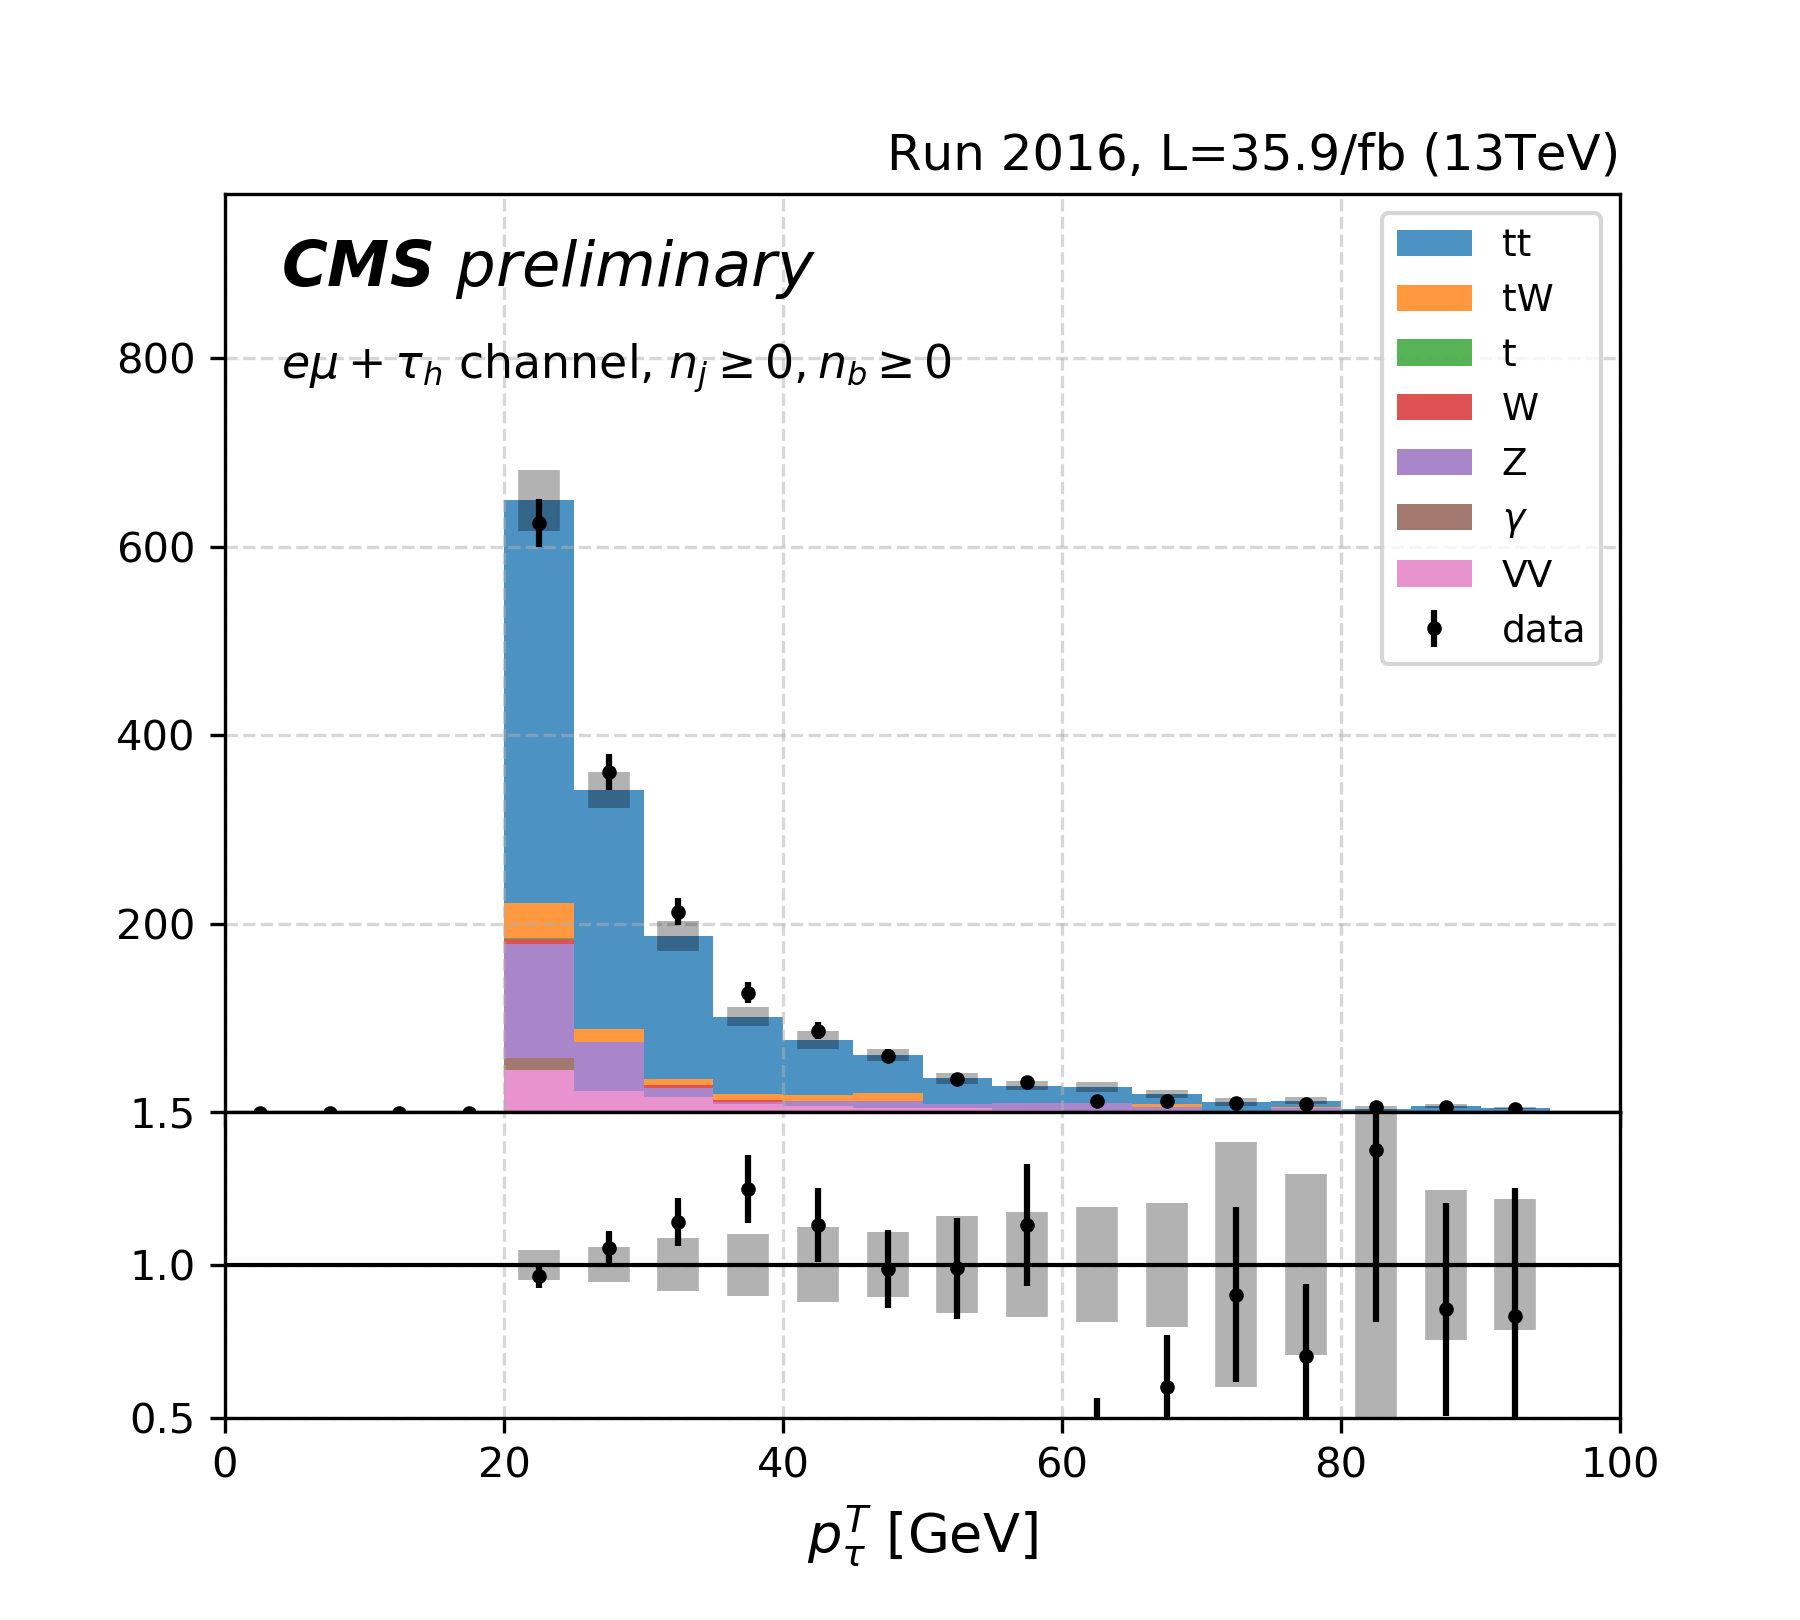
\includegraphics[width=0.32\textwidth]{chapters/Analysis/sectionCalibration/figures/jetToTauh/emutau_tauPt_pickles_lltauVTight.png}
    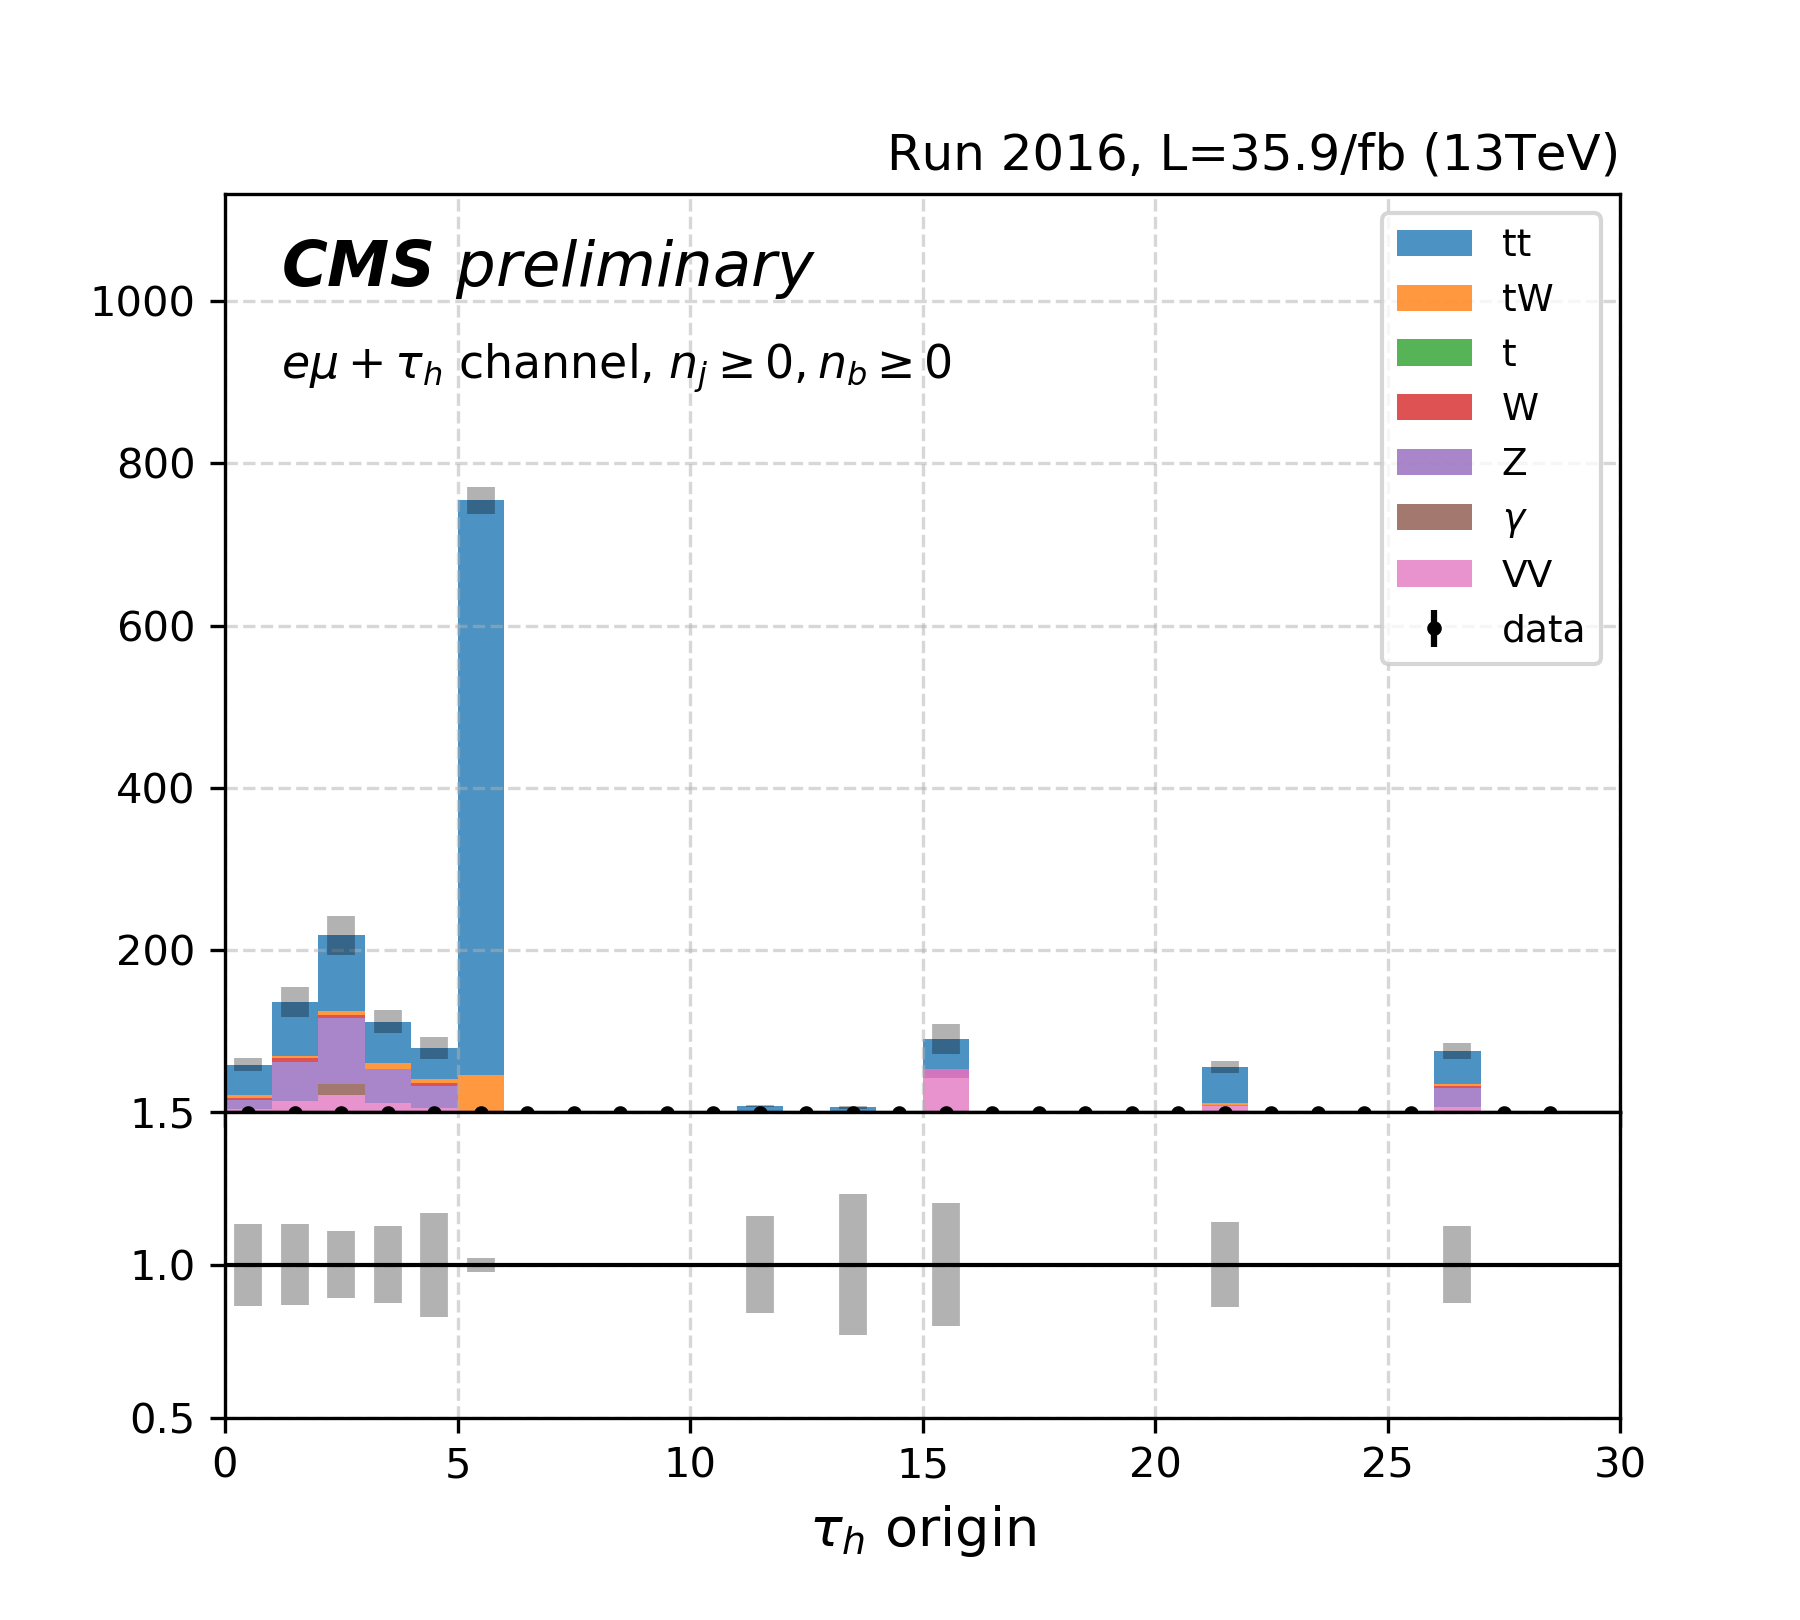
\includegraphics[width=0.32\textwidth]{chapters/Analysis/sectionCalibration/figures/jetToTauh/emutau_tauGenFlavor_pickles_lltauVTight.png}
    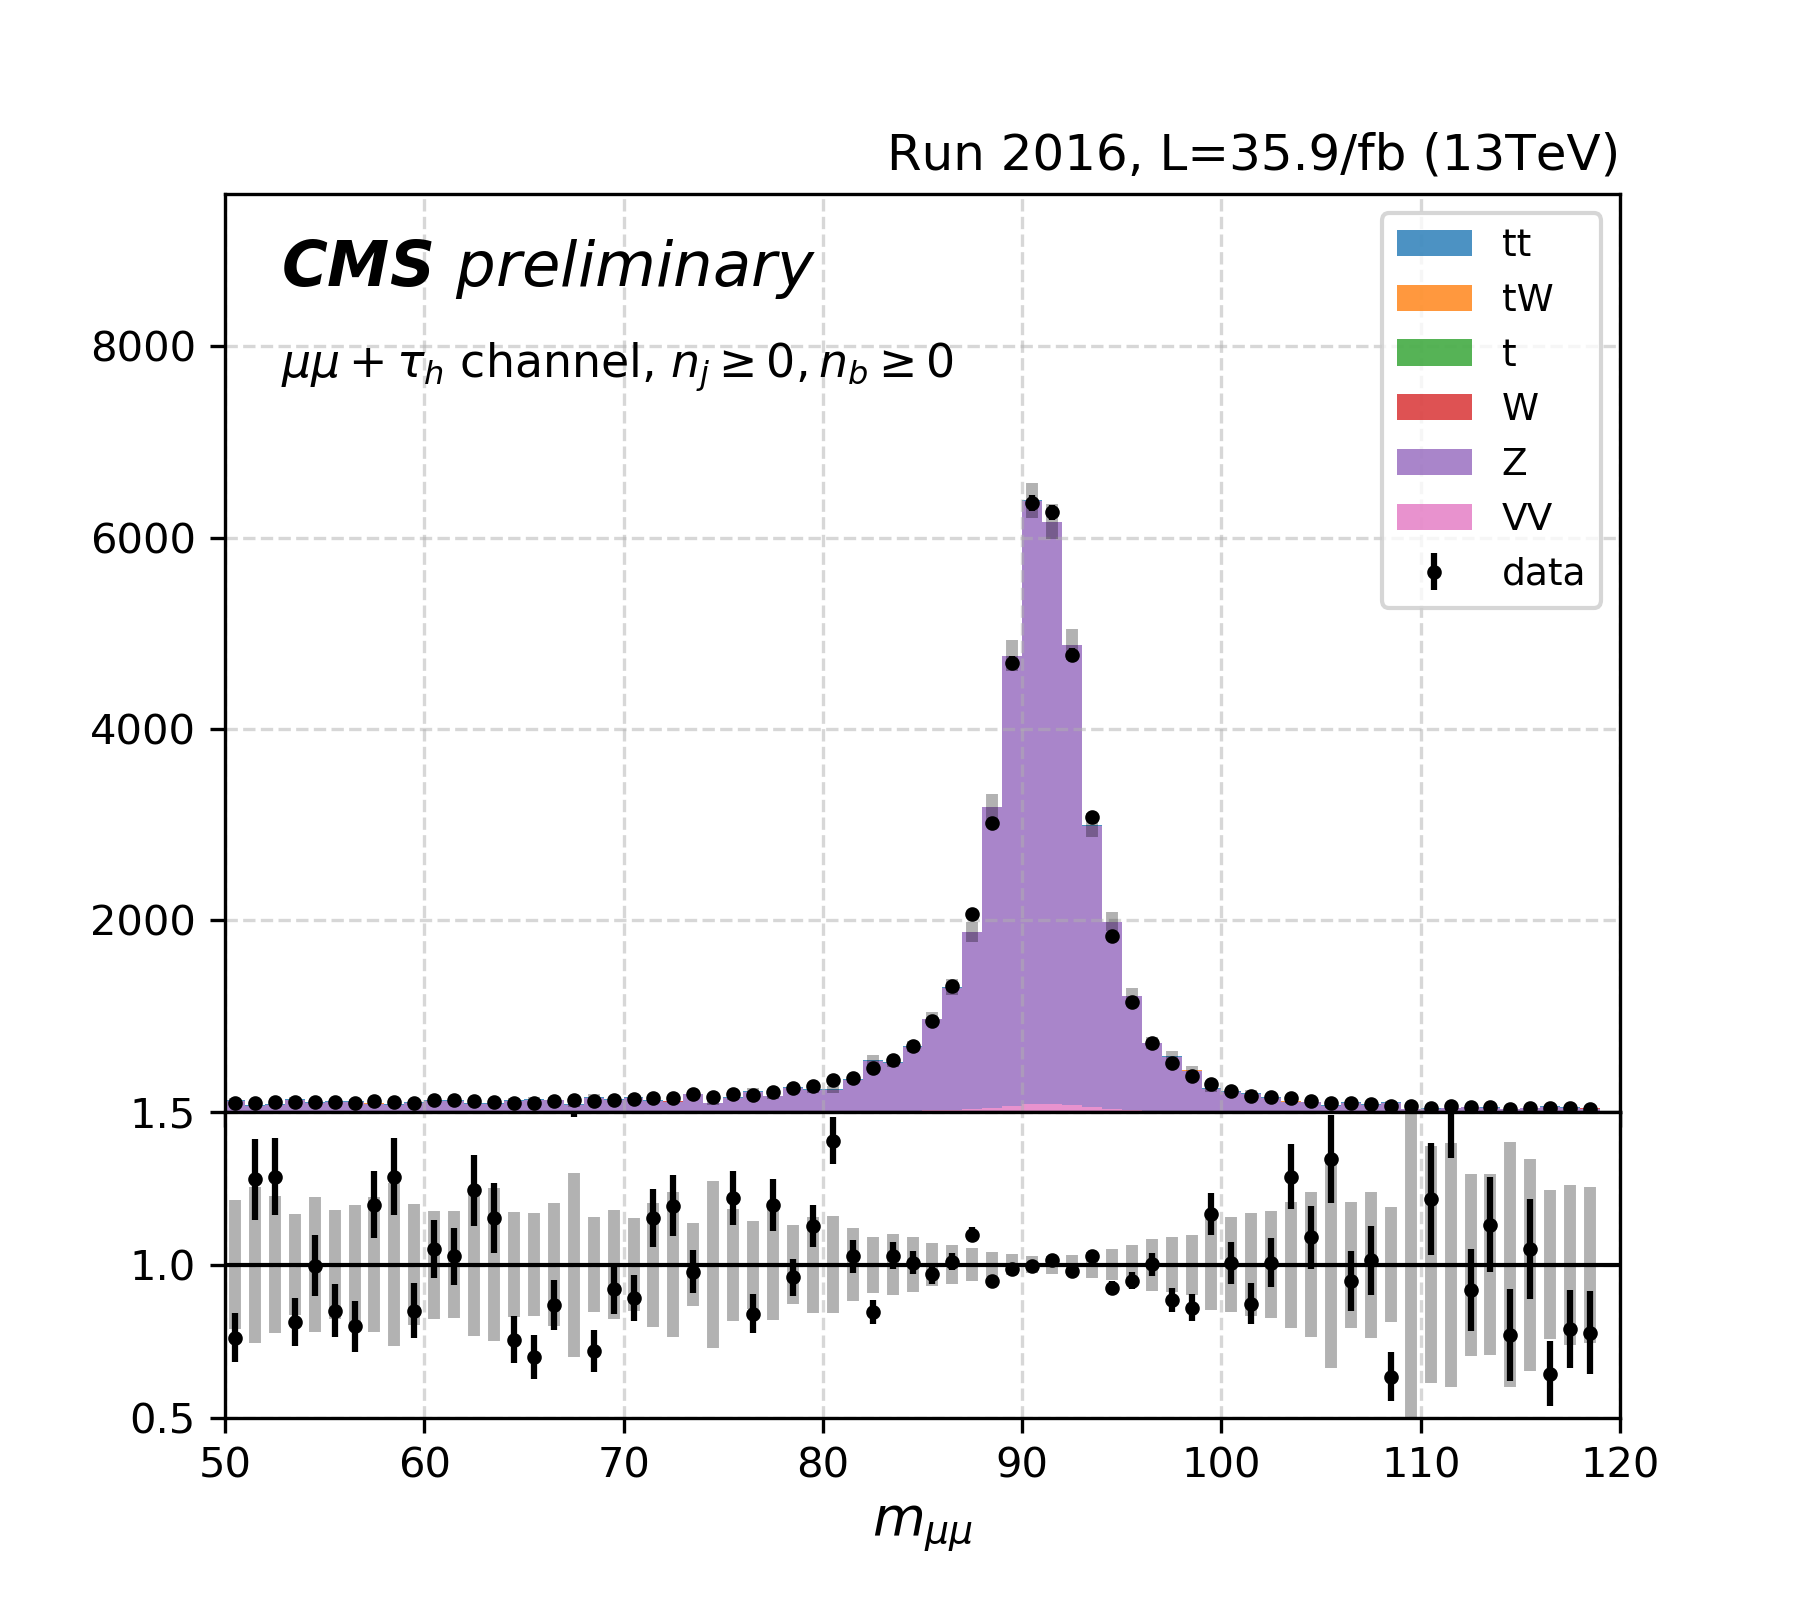
\includegraphics[width=0.32\textwidth]{chapters/Analysis/sectionCalibration/figures/jetToTauh/mumutau_dilepton_mass_pickles_lltauVTight.png}
    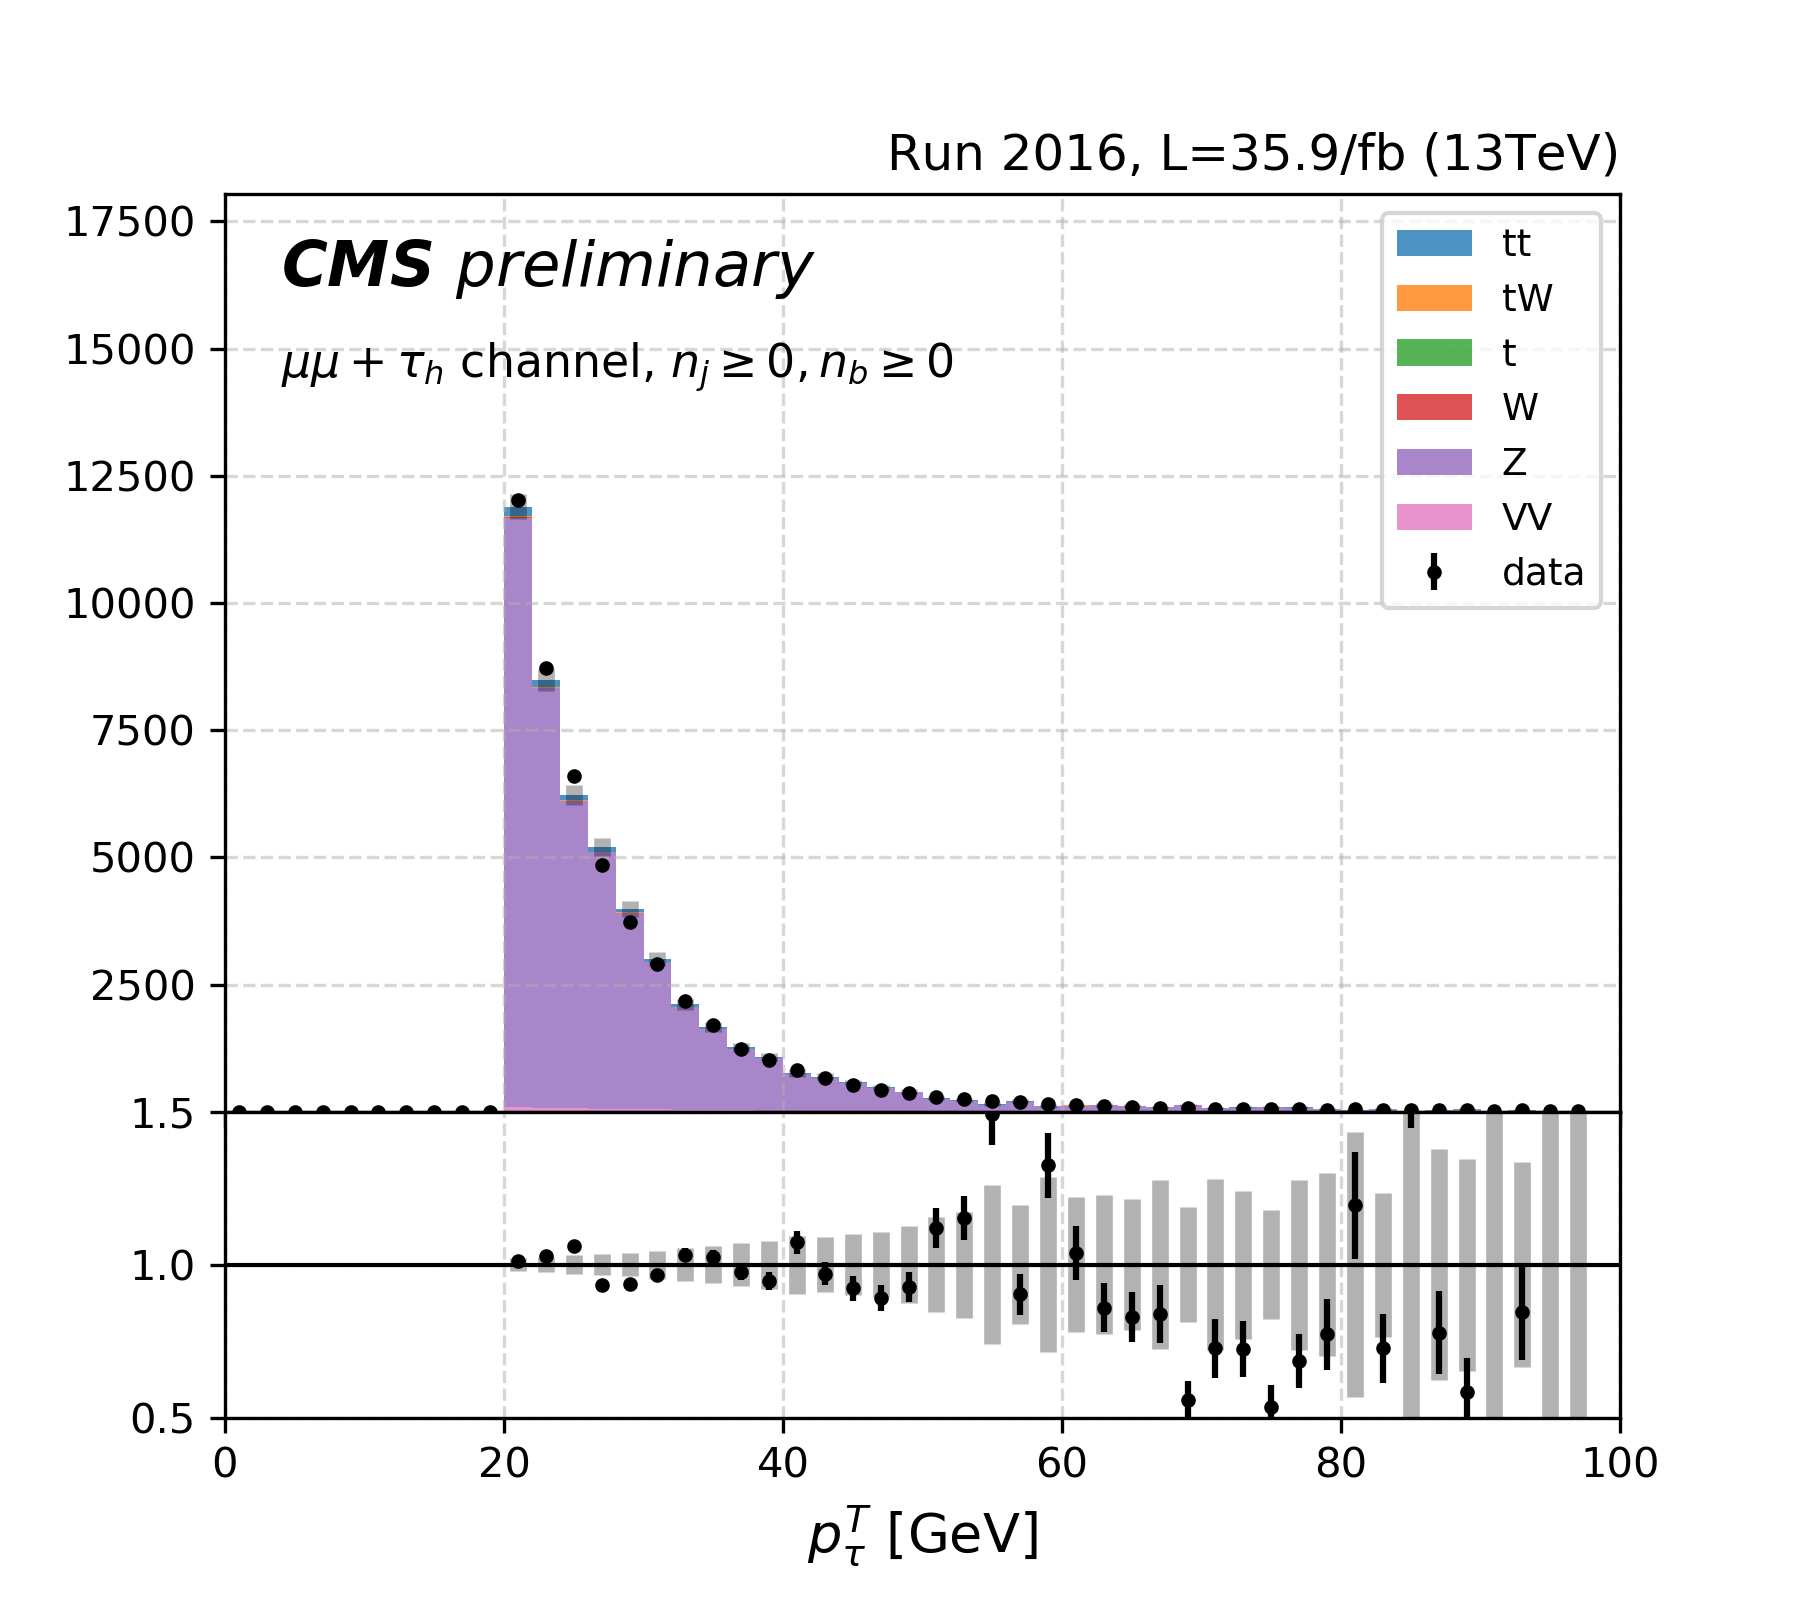
\includegraphics[width=0.32\textwidth]{chapters/Analysis/sectionCalibration/figures/jetToTauh/mumutau_tauPt_pickles_lltauVTight.png}
    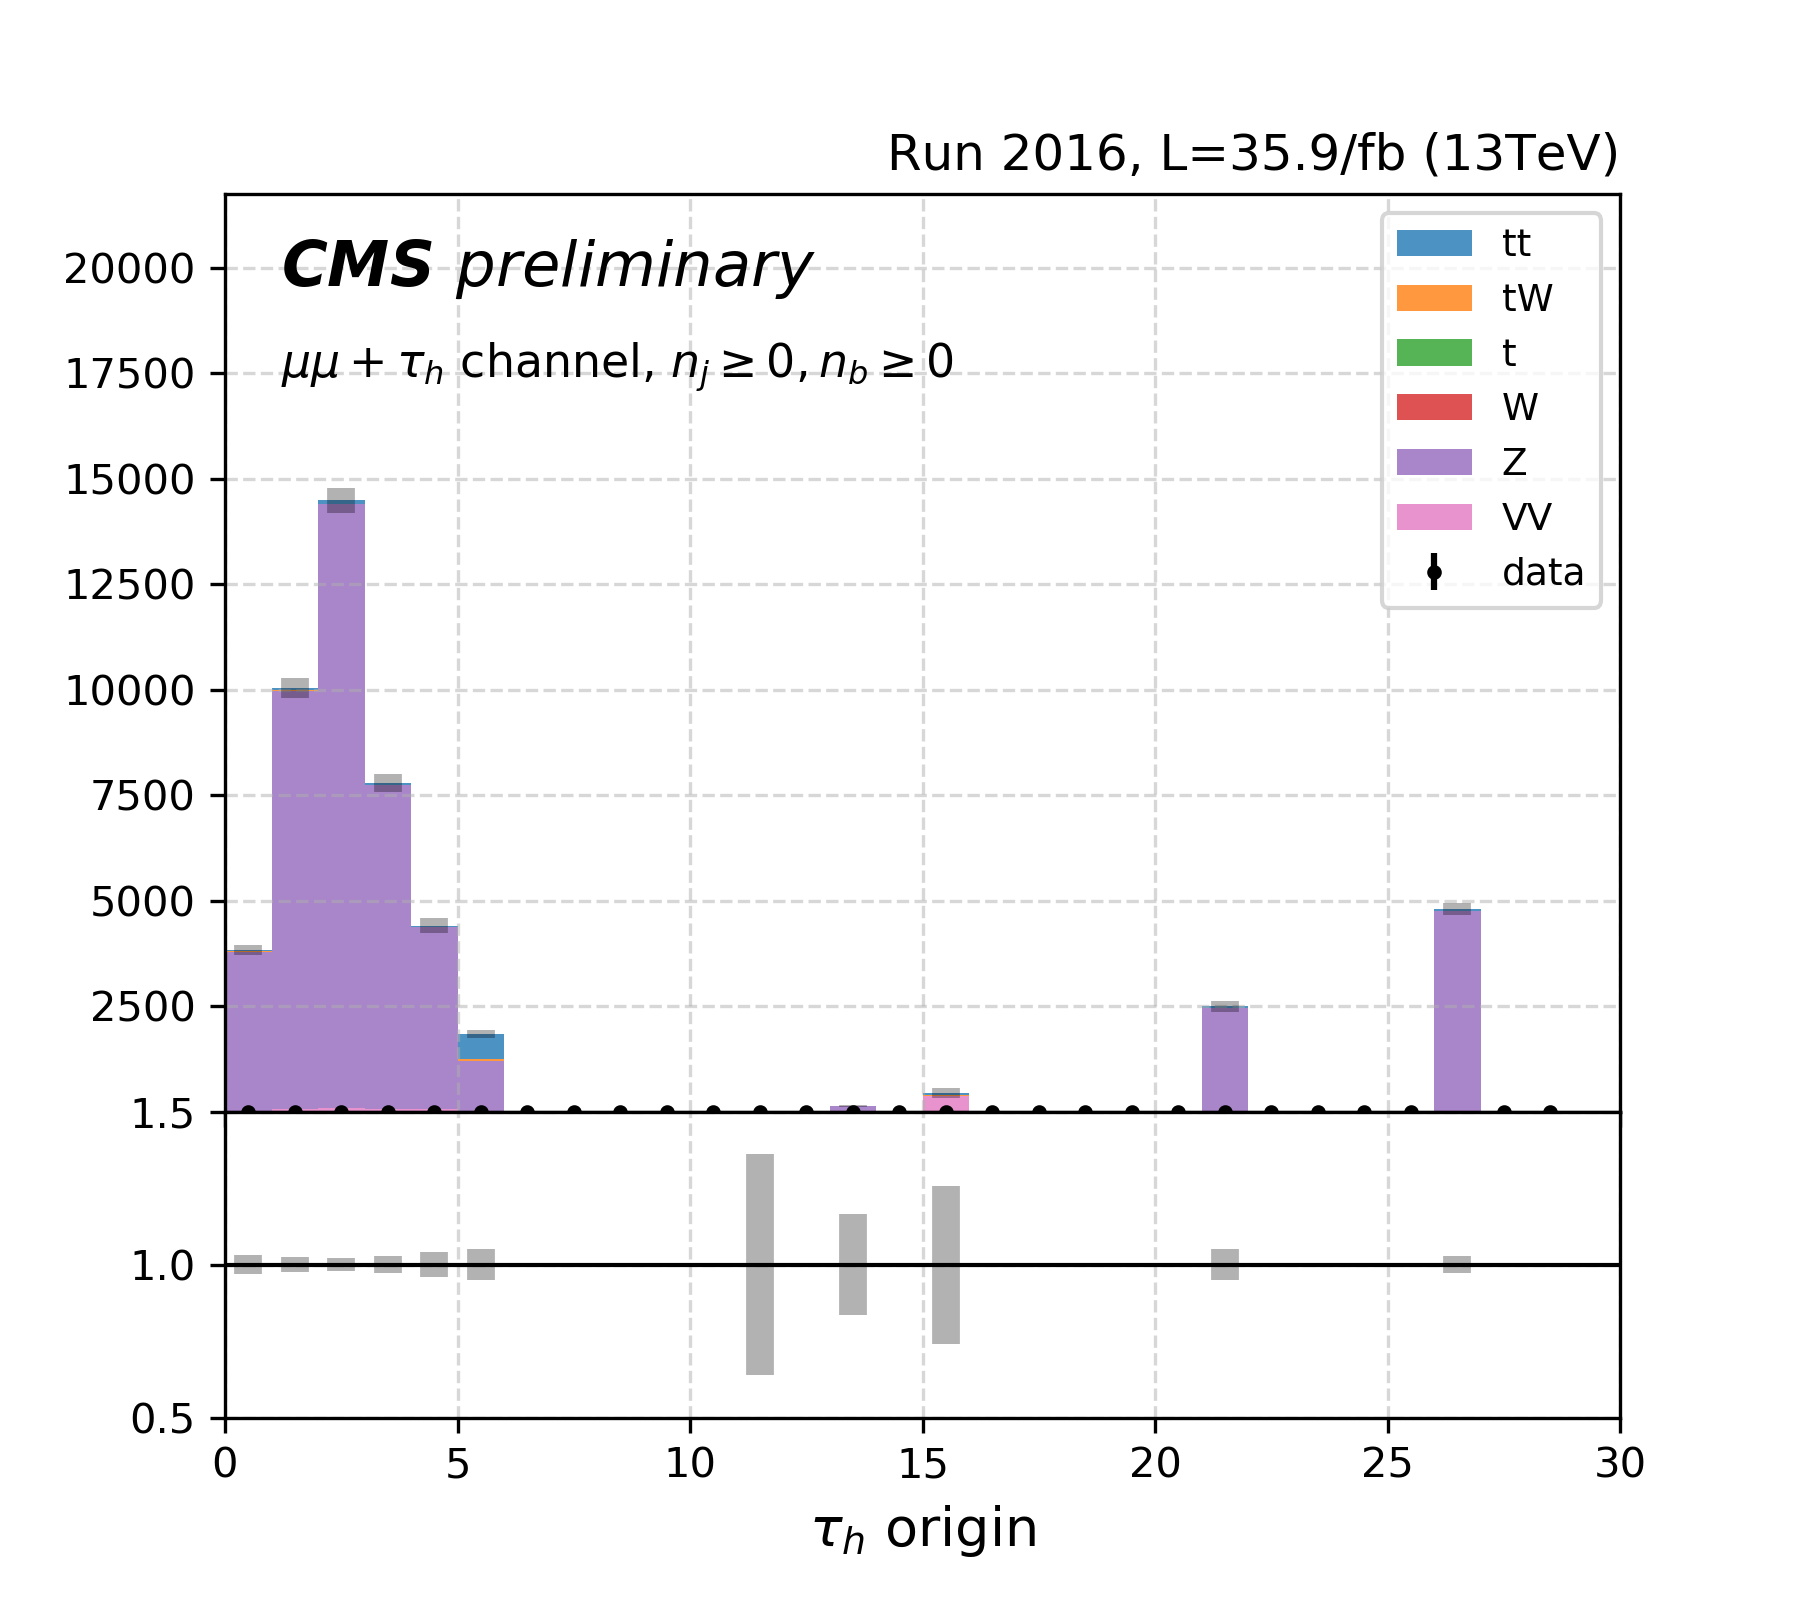
\includegraphics[width=0.32\textwidth]{chapters/Analysis/sectionCalibration/figures/jetToTauh/mumutau_tauGenFlavor_pickles_lltauVTight.png}
    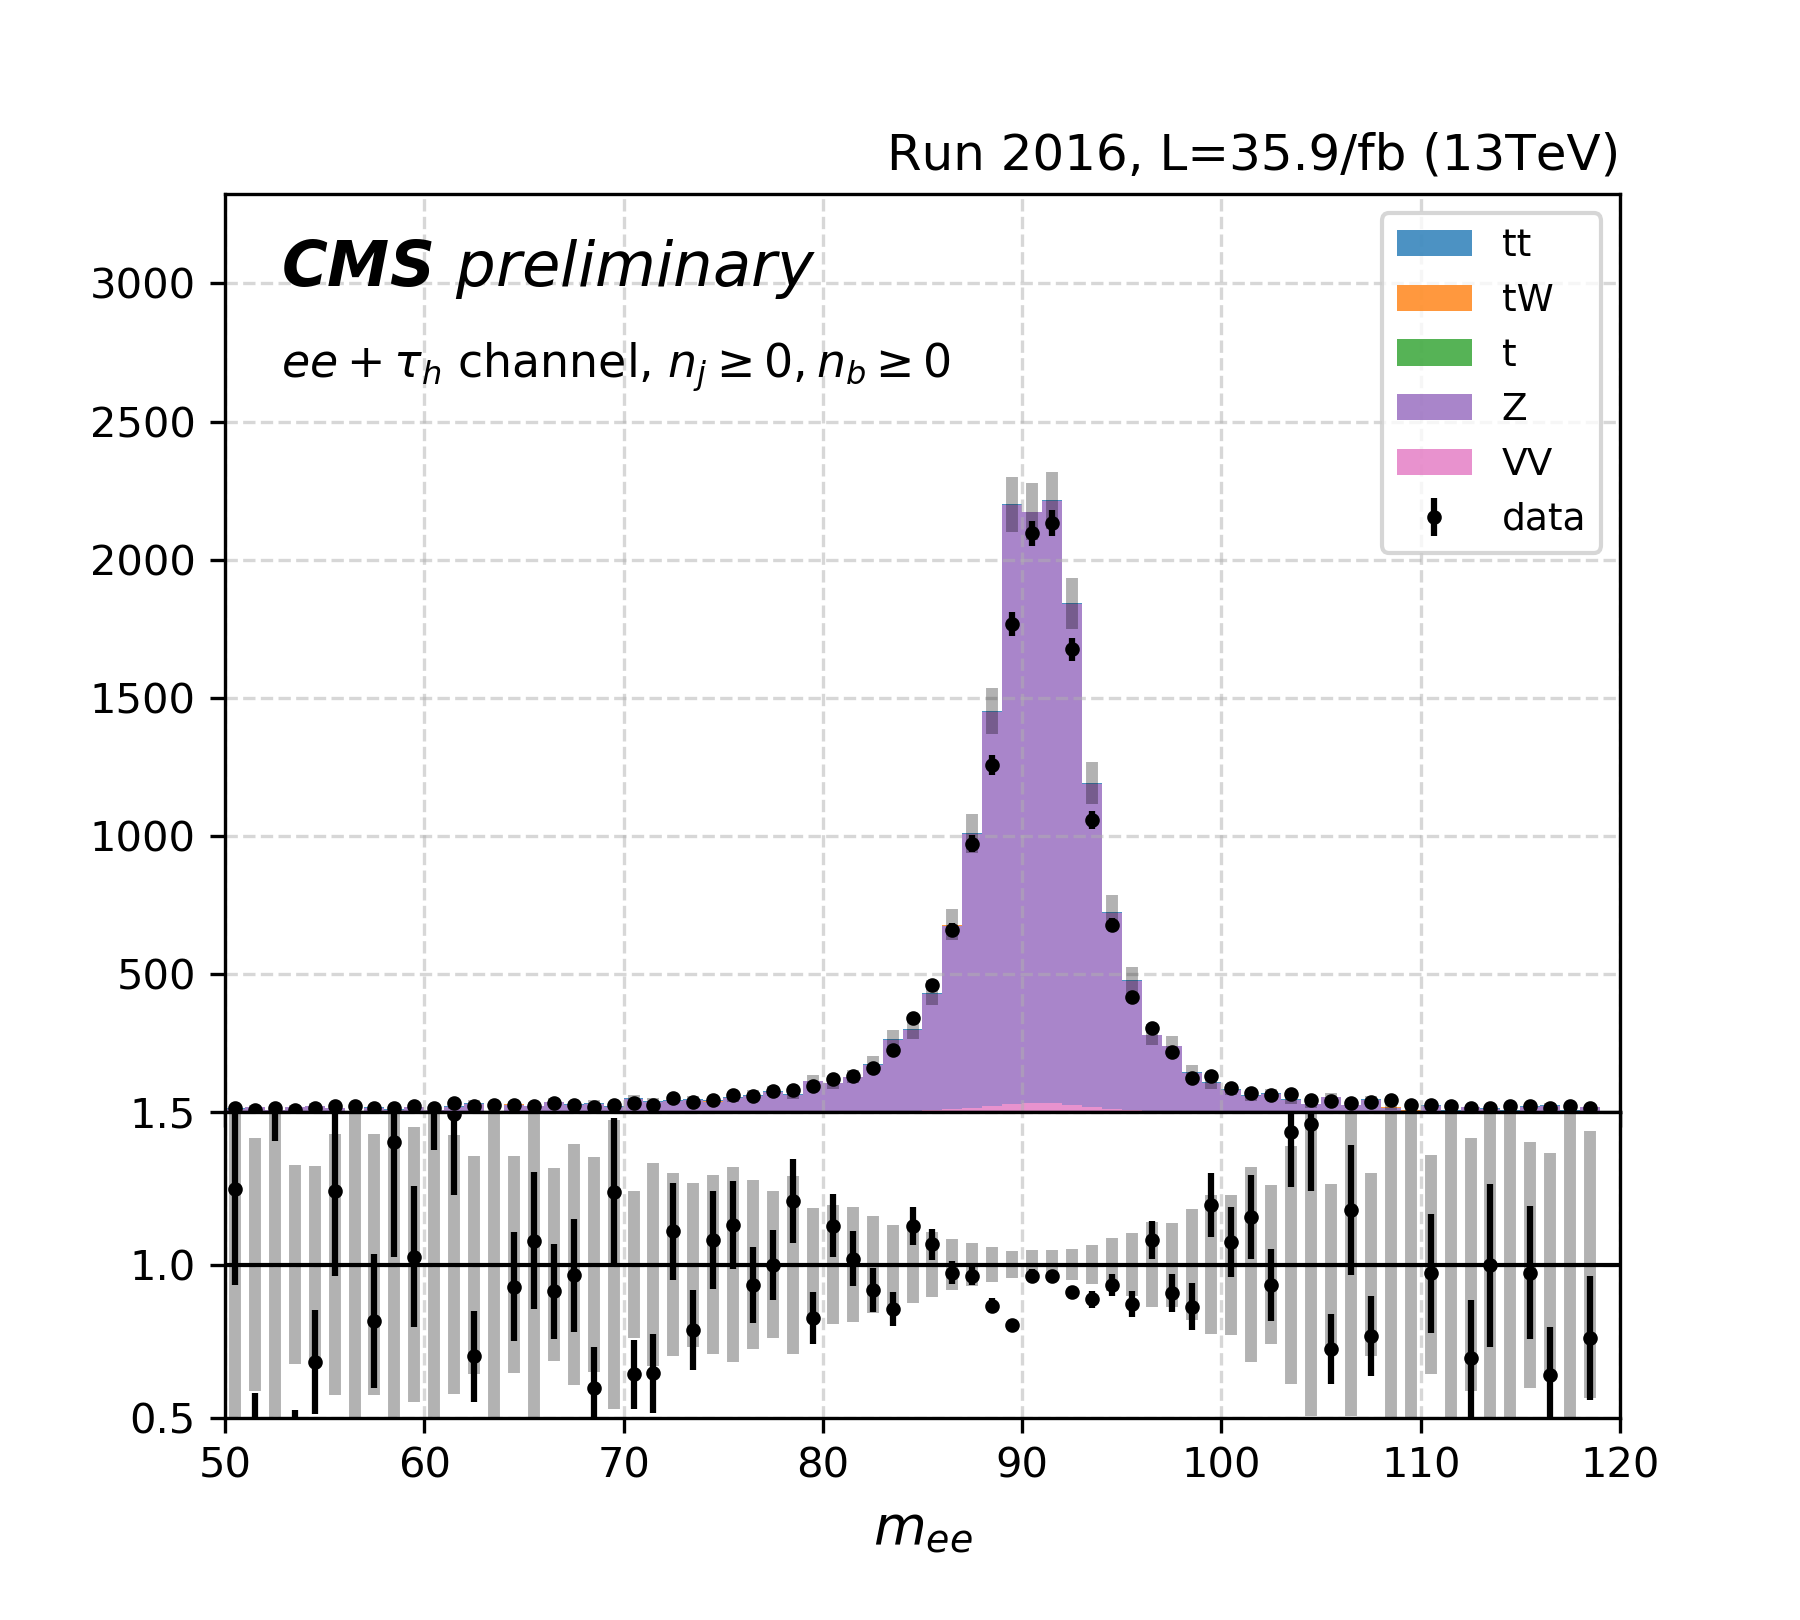
\includegraphics[width=0.32\textwidth]{chapters/Analysis/sectionCalibration/figures/jetToTauh/eetau_dilepton_mass_pickles_lltauVTight.png}
    \includegraphics[width=0.32\textwidth]{chapters/Analysis/sectionCalibration/figures/jetToTauh/eetau_tauPt_pickles_lltauvTight.png}
    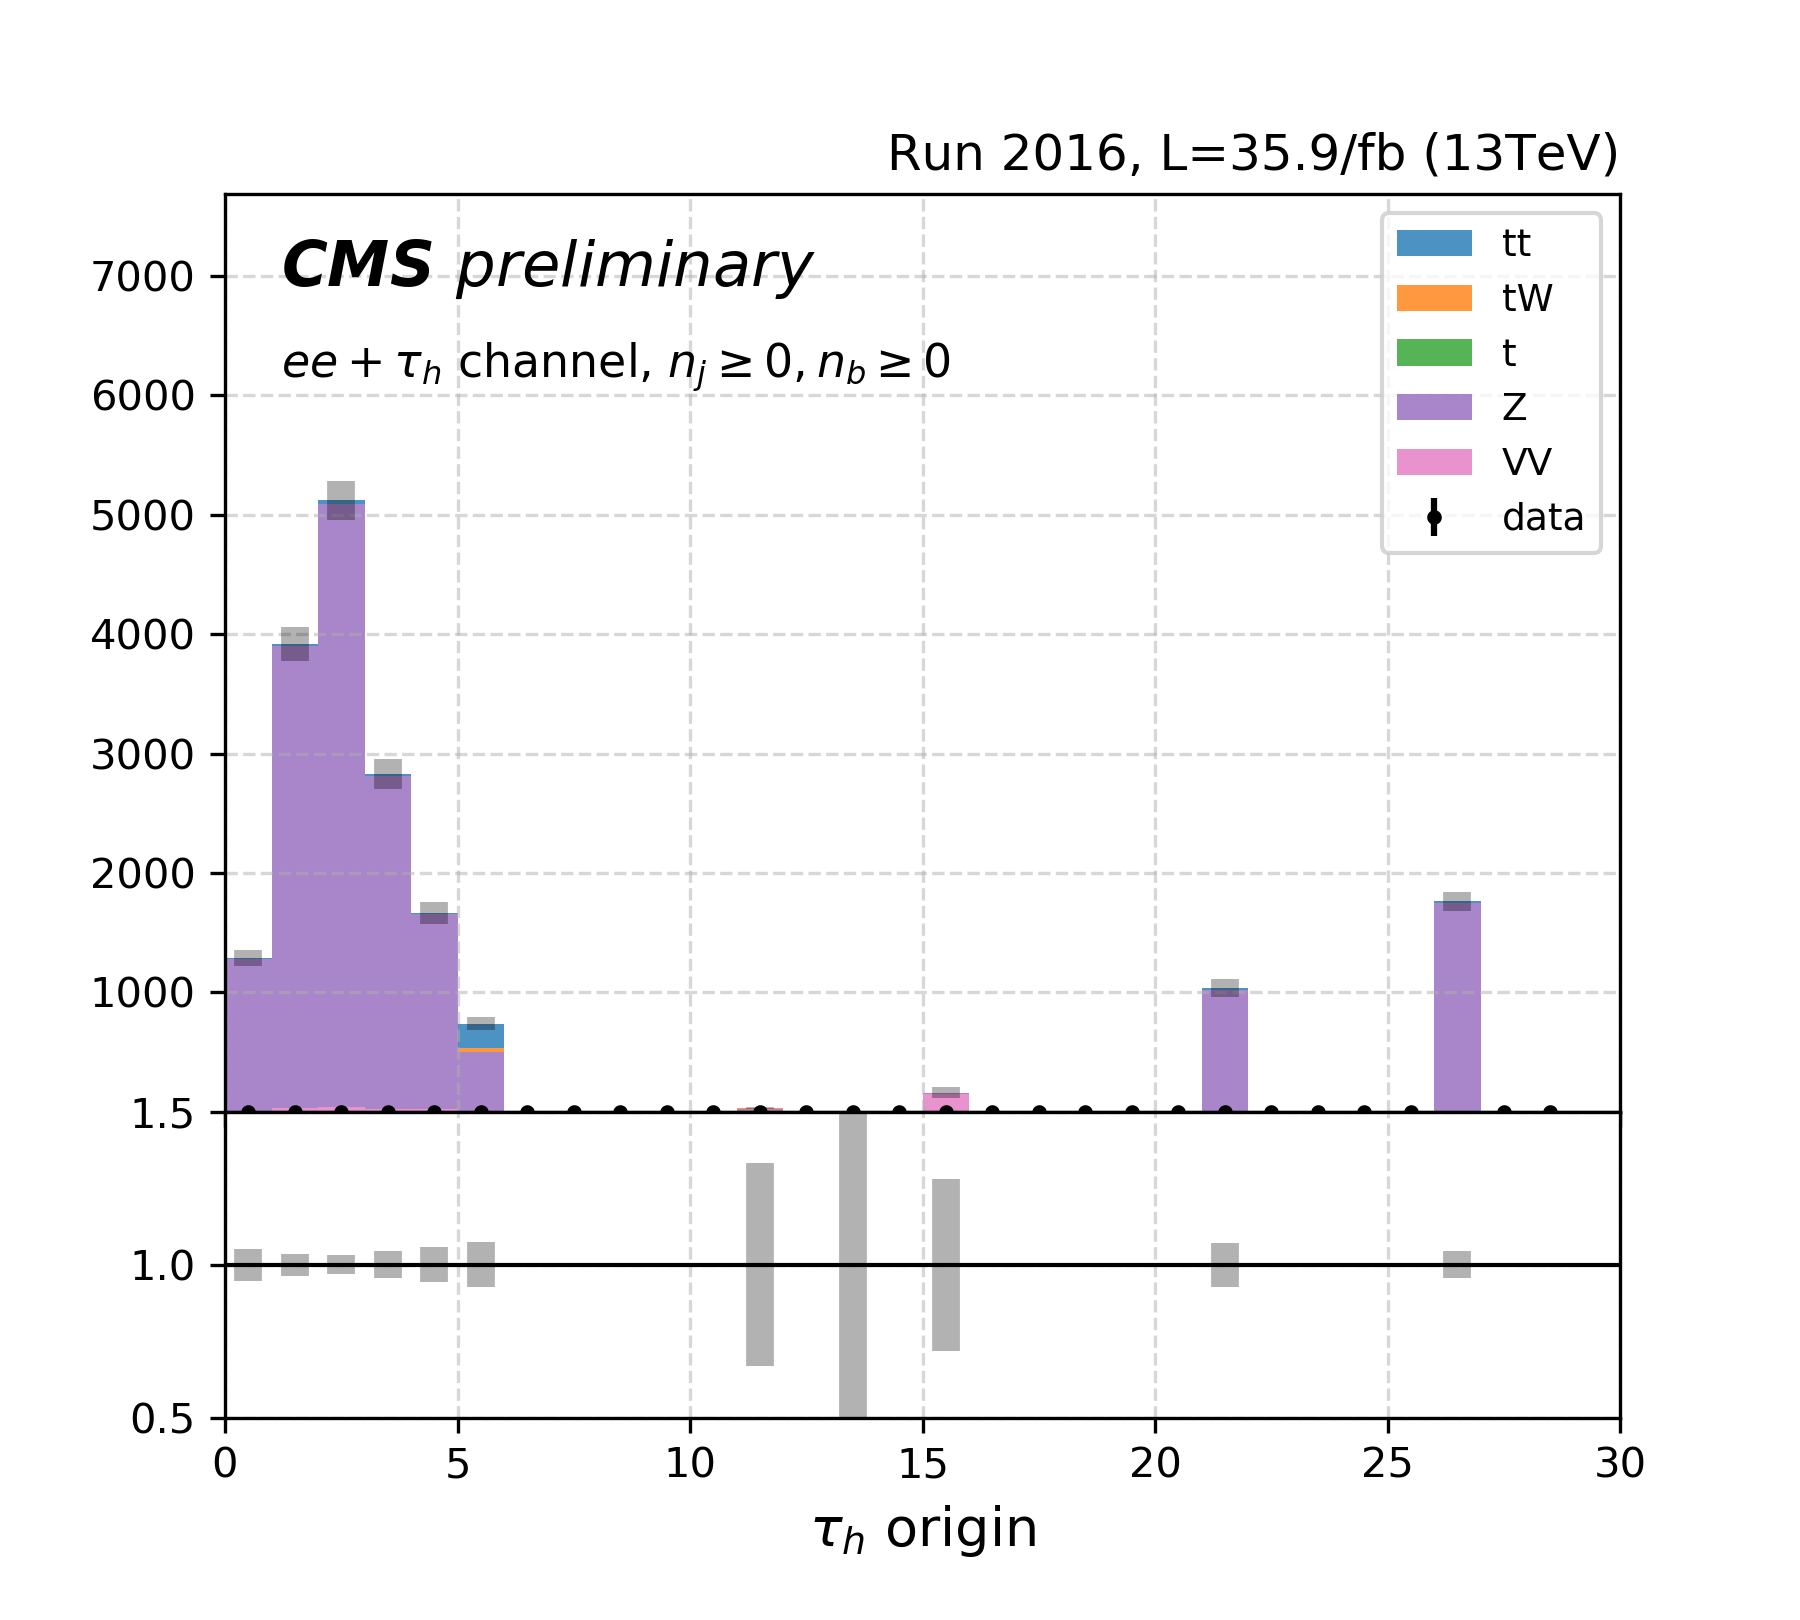
\includegraphics[width=0.32\textwidth]{chapters/Analysis/sectionCalibration/figures/jetToTauh/eetau_tauGenFlavor_pickles_lltauVTight.png}
    \caption{The kinematics distribution of $\cem+\PGth$, $\cmm+\PGth$, $\cee+\PGth$ channels with Very Tight \PGth working point.}
    \label{fig:analysis:calibration:llt_vtight}
\end{figure}



% The \PGth \pt in $\cmm+\PGth$, $\cee+\PGth$ and $\cem+\PGth$ channels are shown in figure~\ref{fig:analysis:calibration:llt_prefit}. 
% \begin{figure}
%     \centering
%     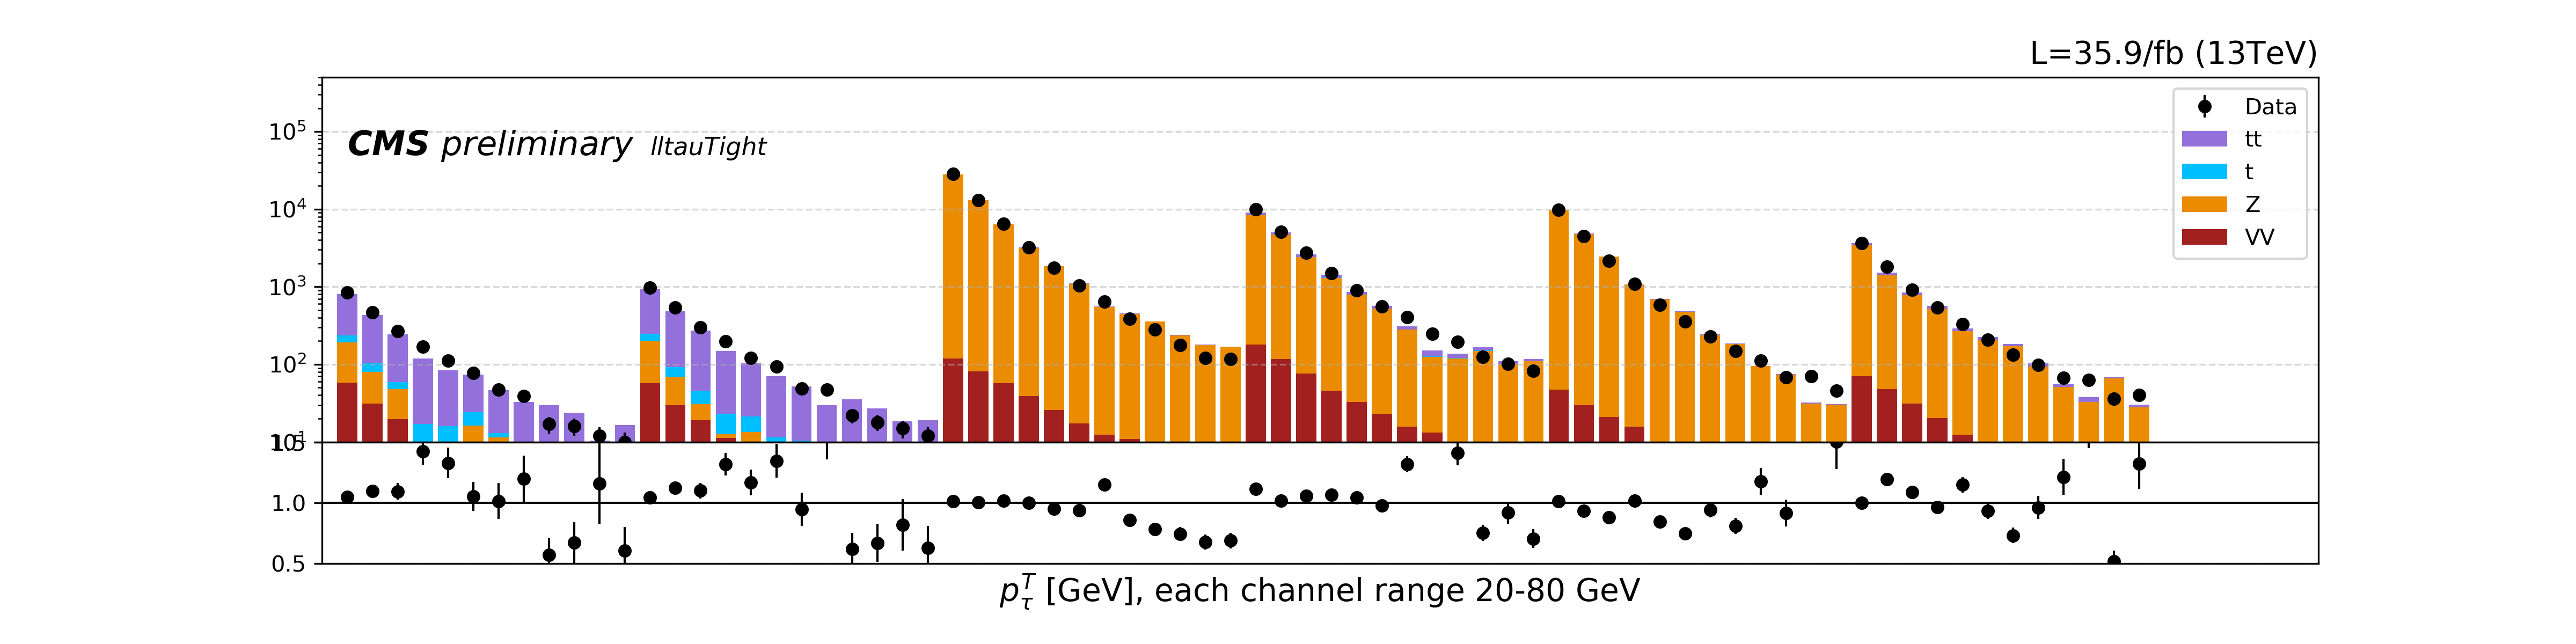
\includegraphics[width=0.99\textwidth]{chapters/Analysis/sectionCalibration/figures/jetToTauh/2020_tauID_prefit_lltauTight.png}
%     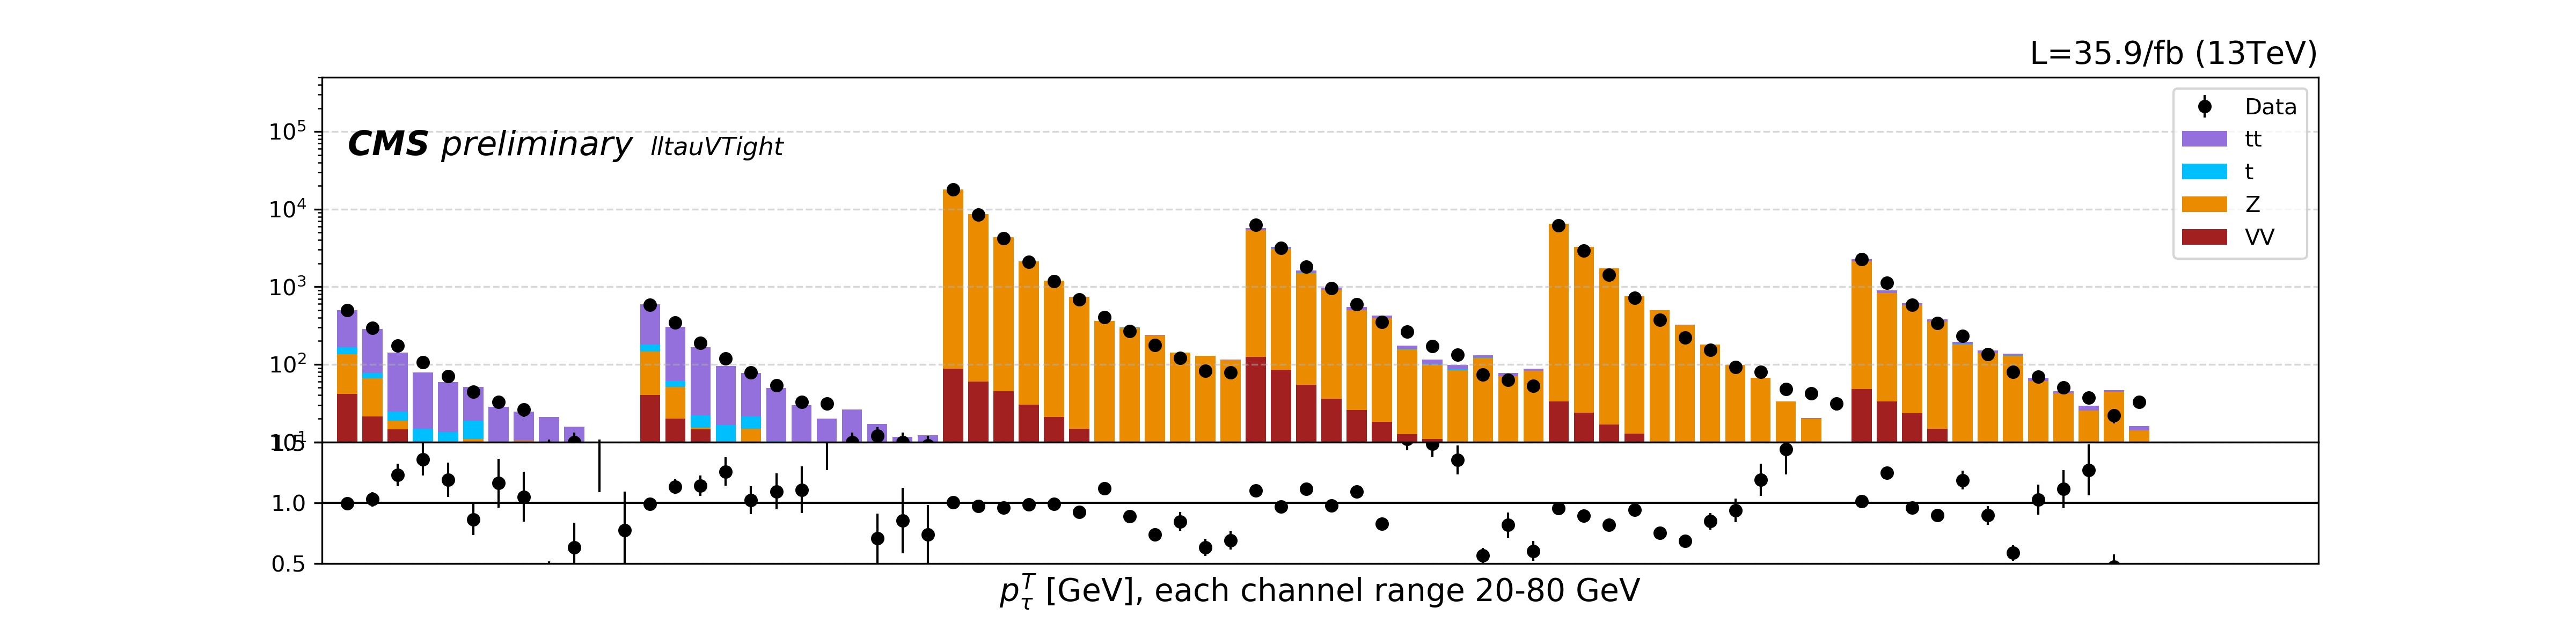
\includegraphics[width=0.99\textwidth]{chapters/Analysis/sectionCalibration/figures/jetToTauh/2020_tauID_prefit_lltauVTight.png}
%     \caption{Prefit distributions of \PGth \pt with Tight \emph{(upper)} and VTight \emph{(lower)} working point.}
%     \label{fig:analysis:calibration:llt_prefit}
% \end{figure}




To measure $SF (\PQq \to \PGth)$  and $SF (\PQb \to \PGth)$, a template fit to the \PGth \pt is performed. The free parameters are $SF (\PQq\to \PGth)$  and $SF (\PQb \to \PGth)$ in 5 \pt bins from 20\GeV to 80\GeV.  The systematical uncertainties, including cross sections, luminosity, electron/muon selection efficiencies, are taken into account as nuisance parameters in the fit.  Because jet modeling of the \zjets simulation is reported to be slightly off in $n_j=0$ but good $n_j \geq 1$, the events are split into $n_j=0$ and $n_j \geq 1$ to deal with jet modeling in the \zjets simulation.  The result of $SF (j\to \PGth)$ for Tight and VTight \PGth working points are listed in Table~\ref{tab:analysis:calibration:takeTauID_result}. Figure~\ref{fig:analysis:calibration:takeTauID_result} shows the measured $SF (j\to \PGth)$ together with pulls and correlation matrix from the template fit.
\begin{table}[h]
    \setlength{\tabcolsep}{6pt} % Default value: 6pt
    \renewcommand{\arraystretch}{1.5} % Default value: 1
    \caption{ Scale factors of $(j\to \PGth)$ with Tight and Very Tight \PGth  working point.}
    \begin{tabular}{c|ccccc}
    \hline
    $p^T_{\PGth}$ [\GeV]  & 20-25      & 25-30         & 30-40         & 40-50         & 50-80         \\
    \hline
    $SF(\PQb\to \rm{Tight} \; \PGth)$  & $1.02\pm0.12$ & $1.16\pm0.12$ & $1.27\pm0.11$ & $1.21\pm0.13$ & $0.81\pm0.13$ \\
    $SF(\PQq\to \rm{Tight} \;  \PGth)$ & $1.04\pm0.08$ & $0.99\pm0.07$ & $0.99\pm0.06$ & $0.90\pm0.06$ & $0.91\pm0.07$ \\
    \hline
    $SF(\PQb\to \rm{VTight} \; \PGth)$ & $0.97\pm0.14$ & $1.19\pm0.16$ & $1.39\pm0.15$ & $0.96\pm0.14$ & $0.91\pm0.17$ \\
    $SF(\PQq\to \rm{VTight} \; \PGth)$ & $1.02\pm0.08$ & $0.95\pm0.07$ & $0.94\pm0.06$ & $0.89\pm0.07$ & $0.86\pm0.07$ \\
    \hline
    \end{tabular}
    \label{tab:analysis:calibration:takeTauID_result}
\end{table}
\begin{figure}[h]
    \centering
    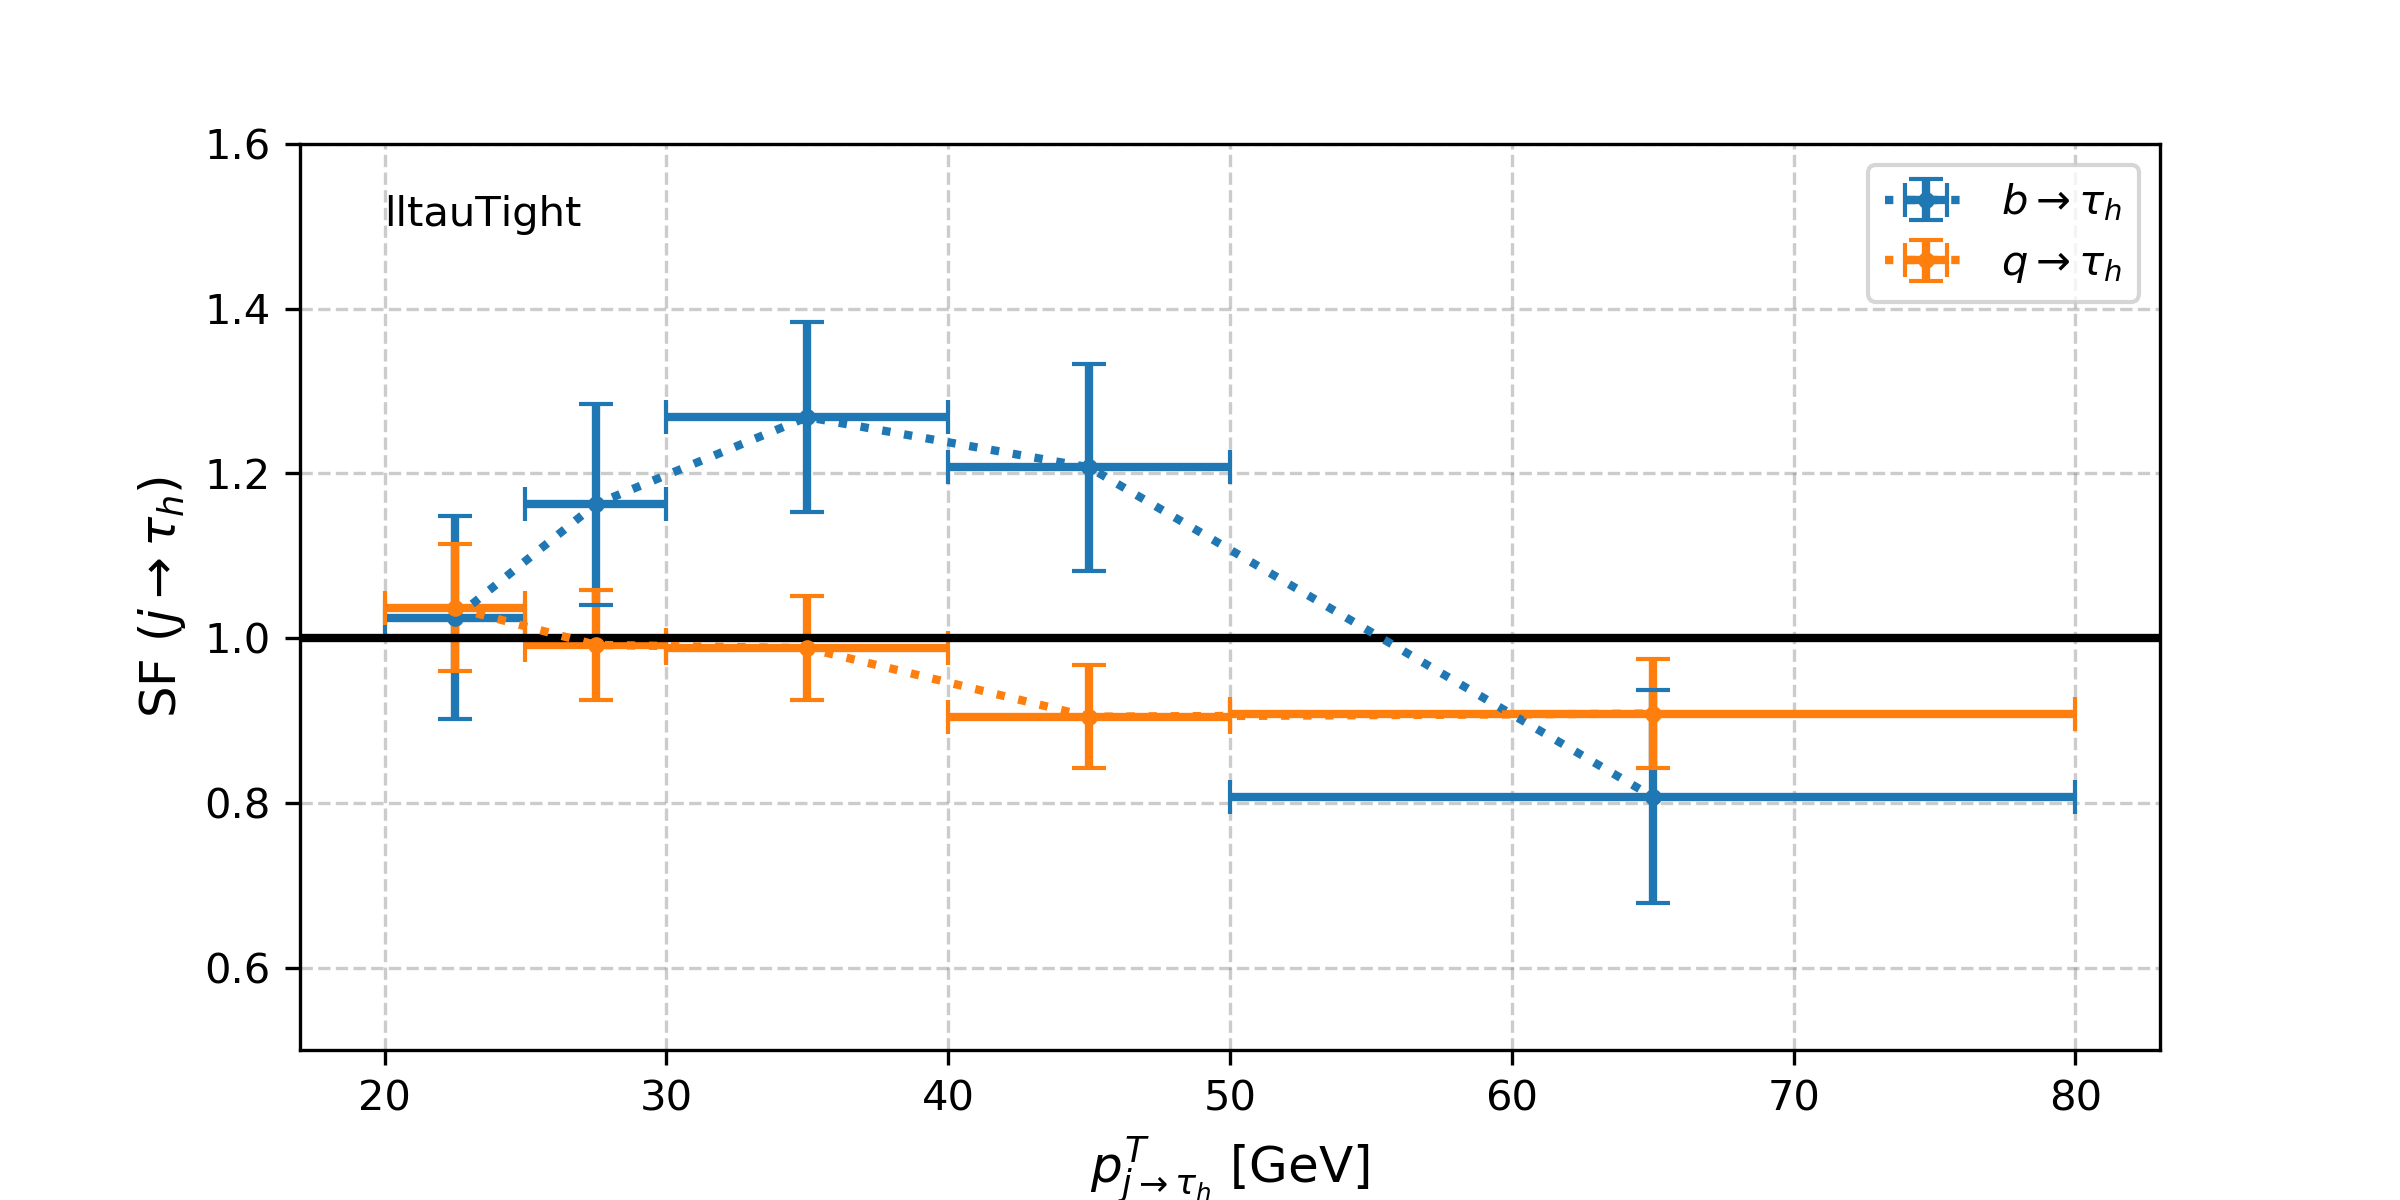
\includegraphics[width=0.49\textwidth]{chapters/Analysis/sectionCalibration/figures/jetToTauh/fit2_ptflavor2_lltauTight.png}
    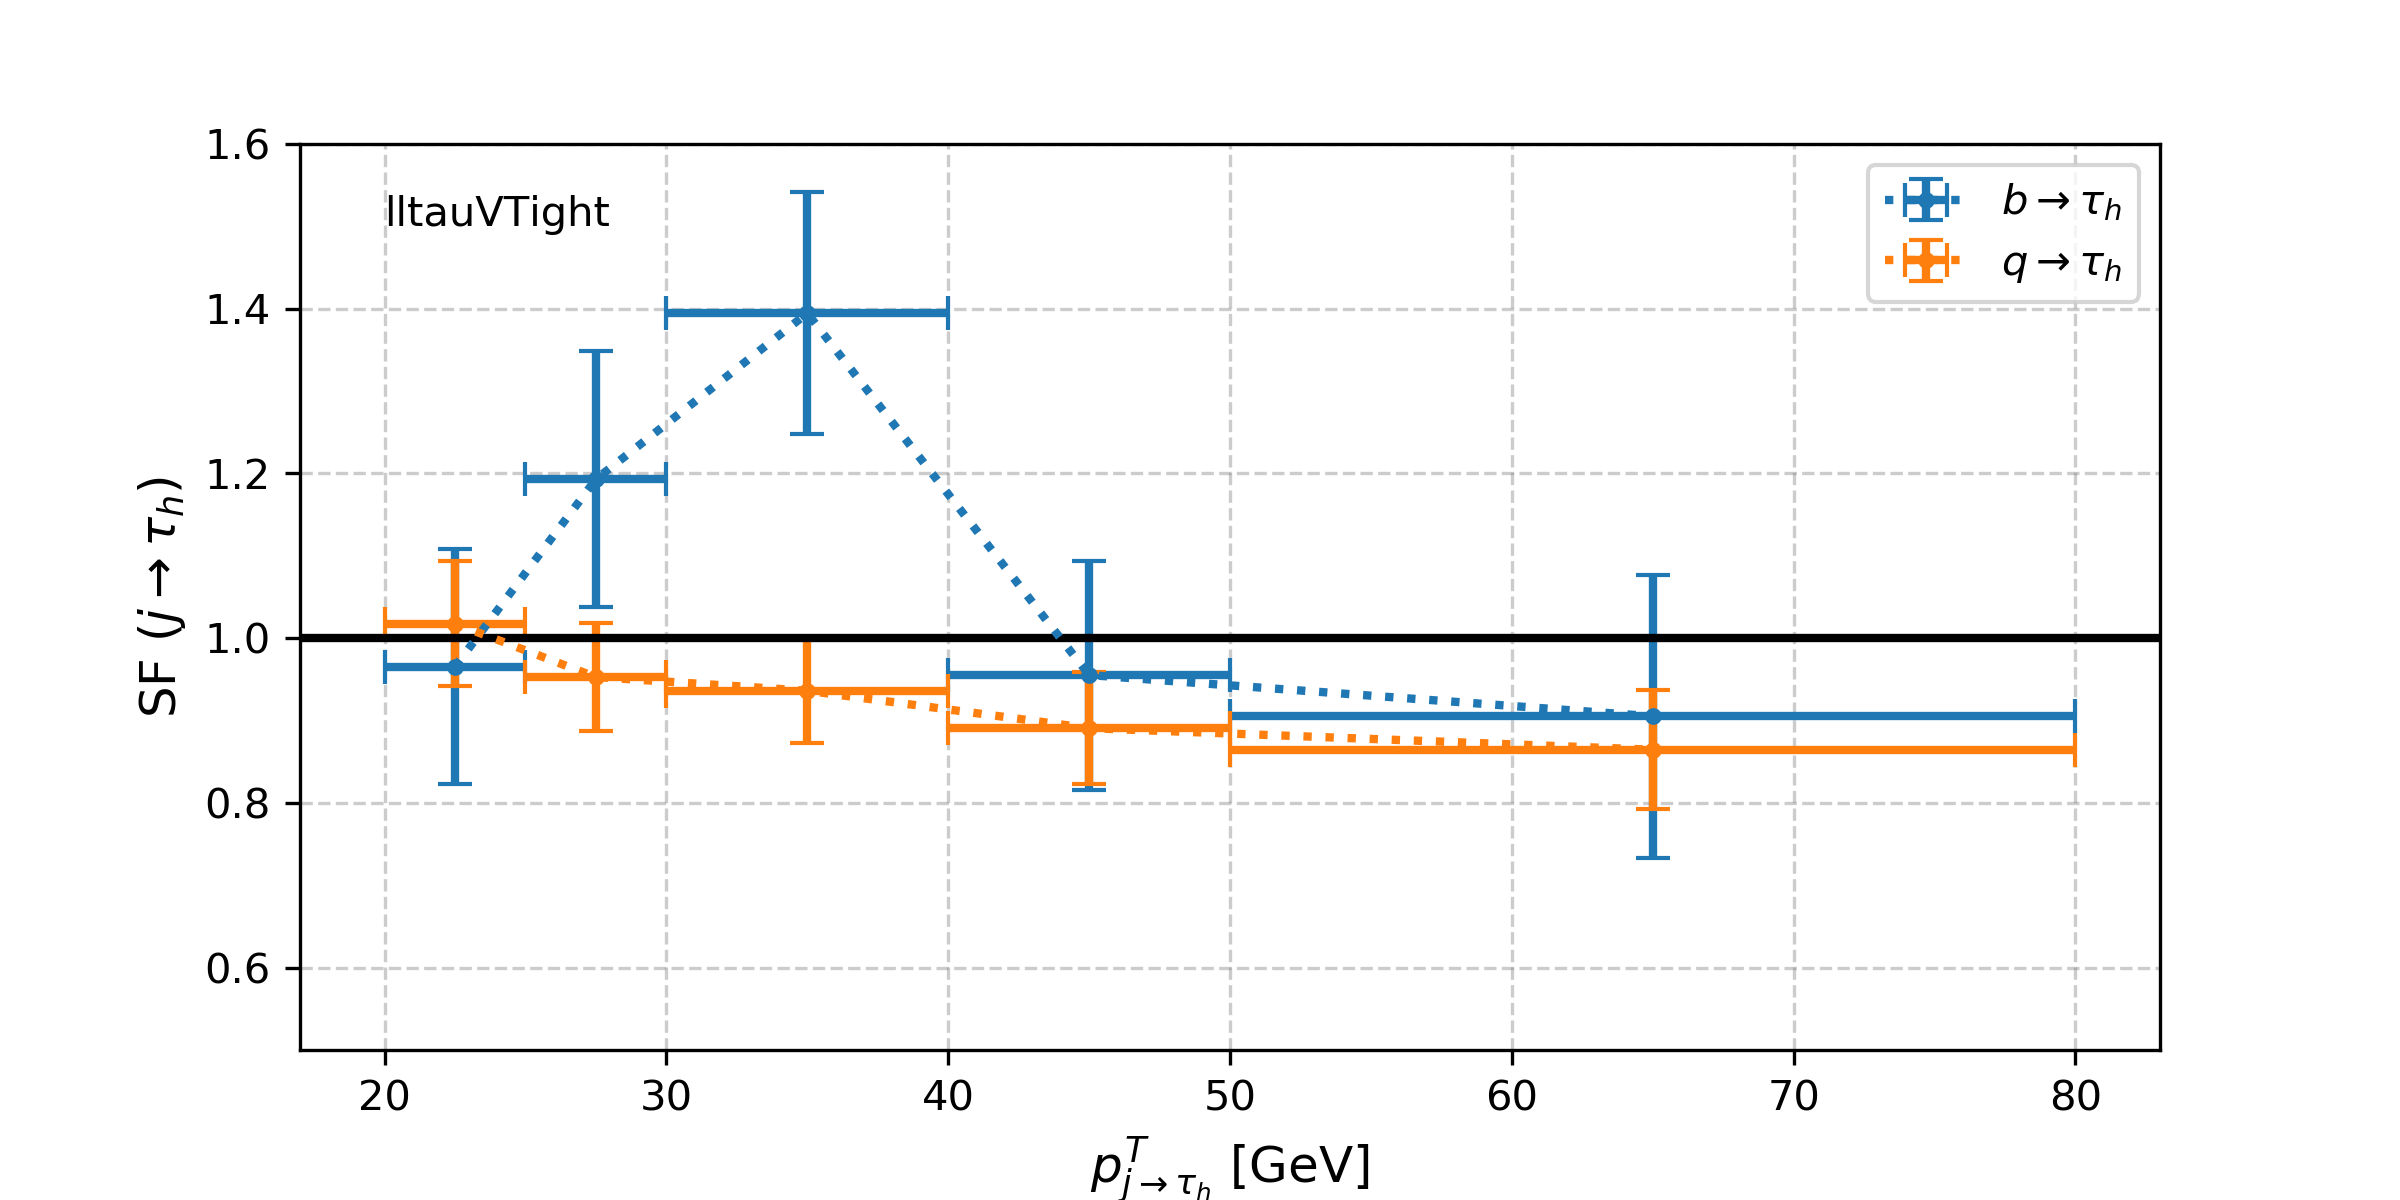
\includegraphics[width=0.49\textwidth]{chapters/Analysis/sectionCalibration/figures/jetToTauh/fit2_ptflavor2_lltauVTight.png}
    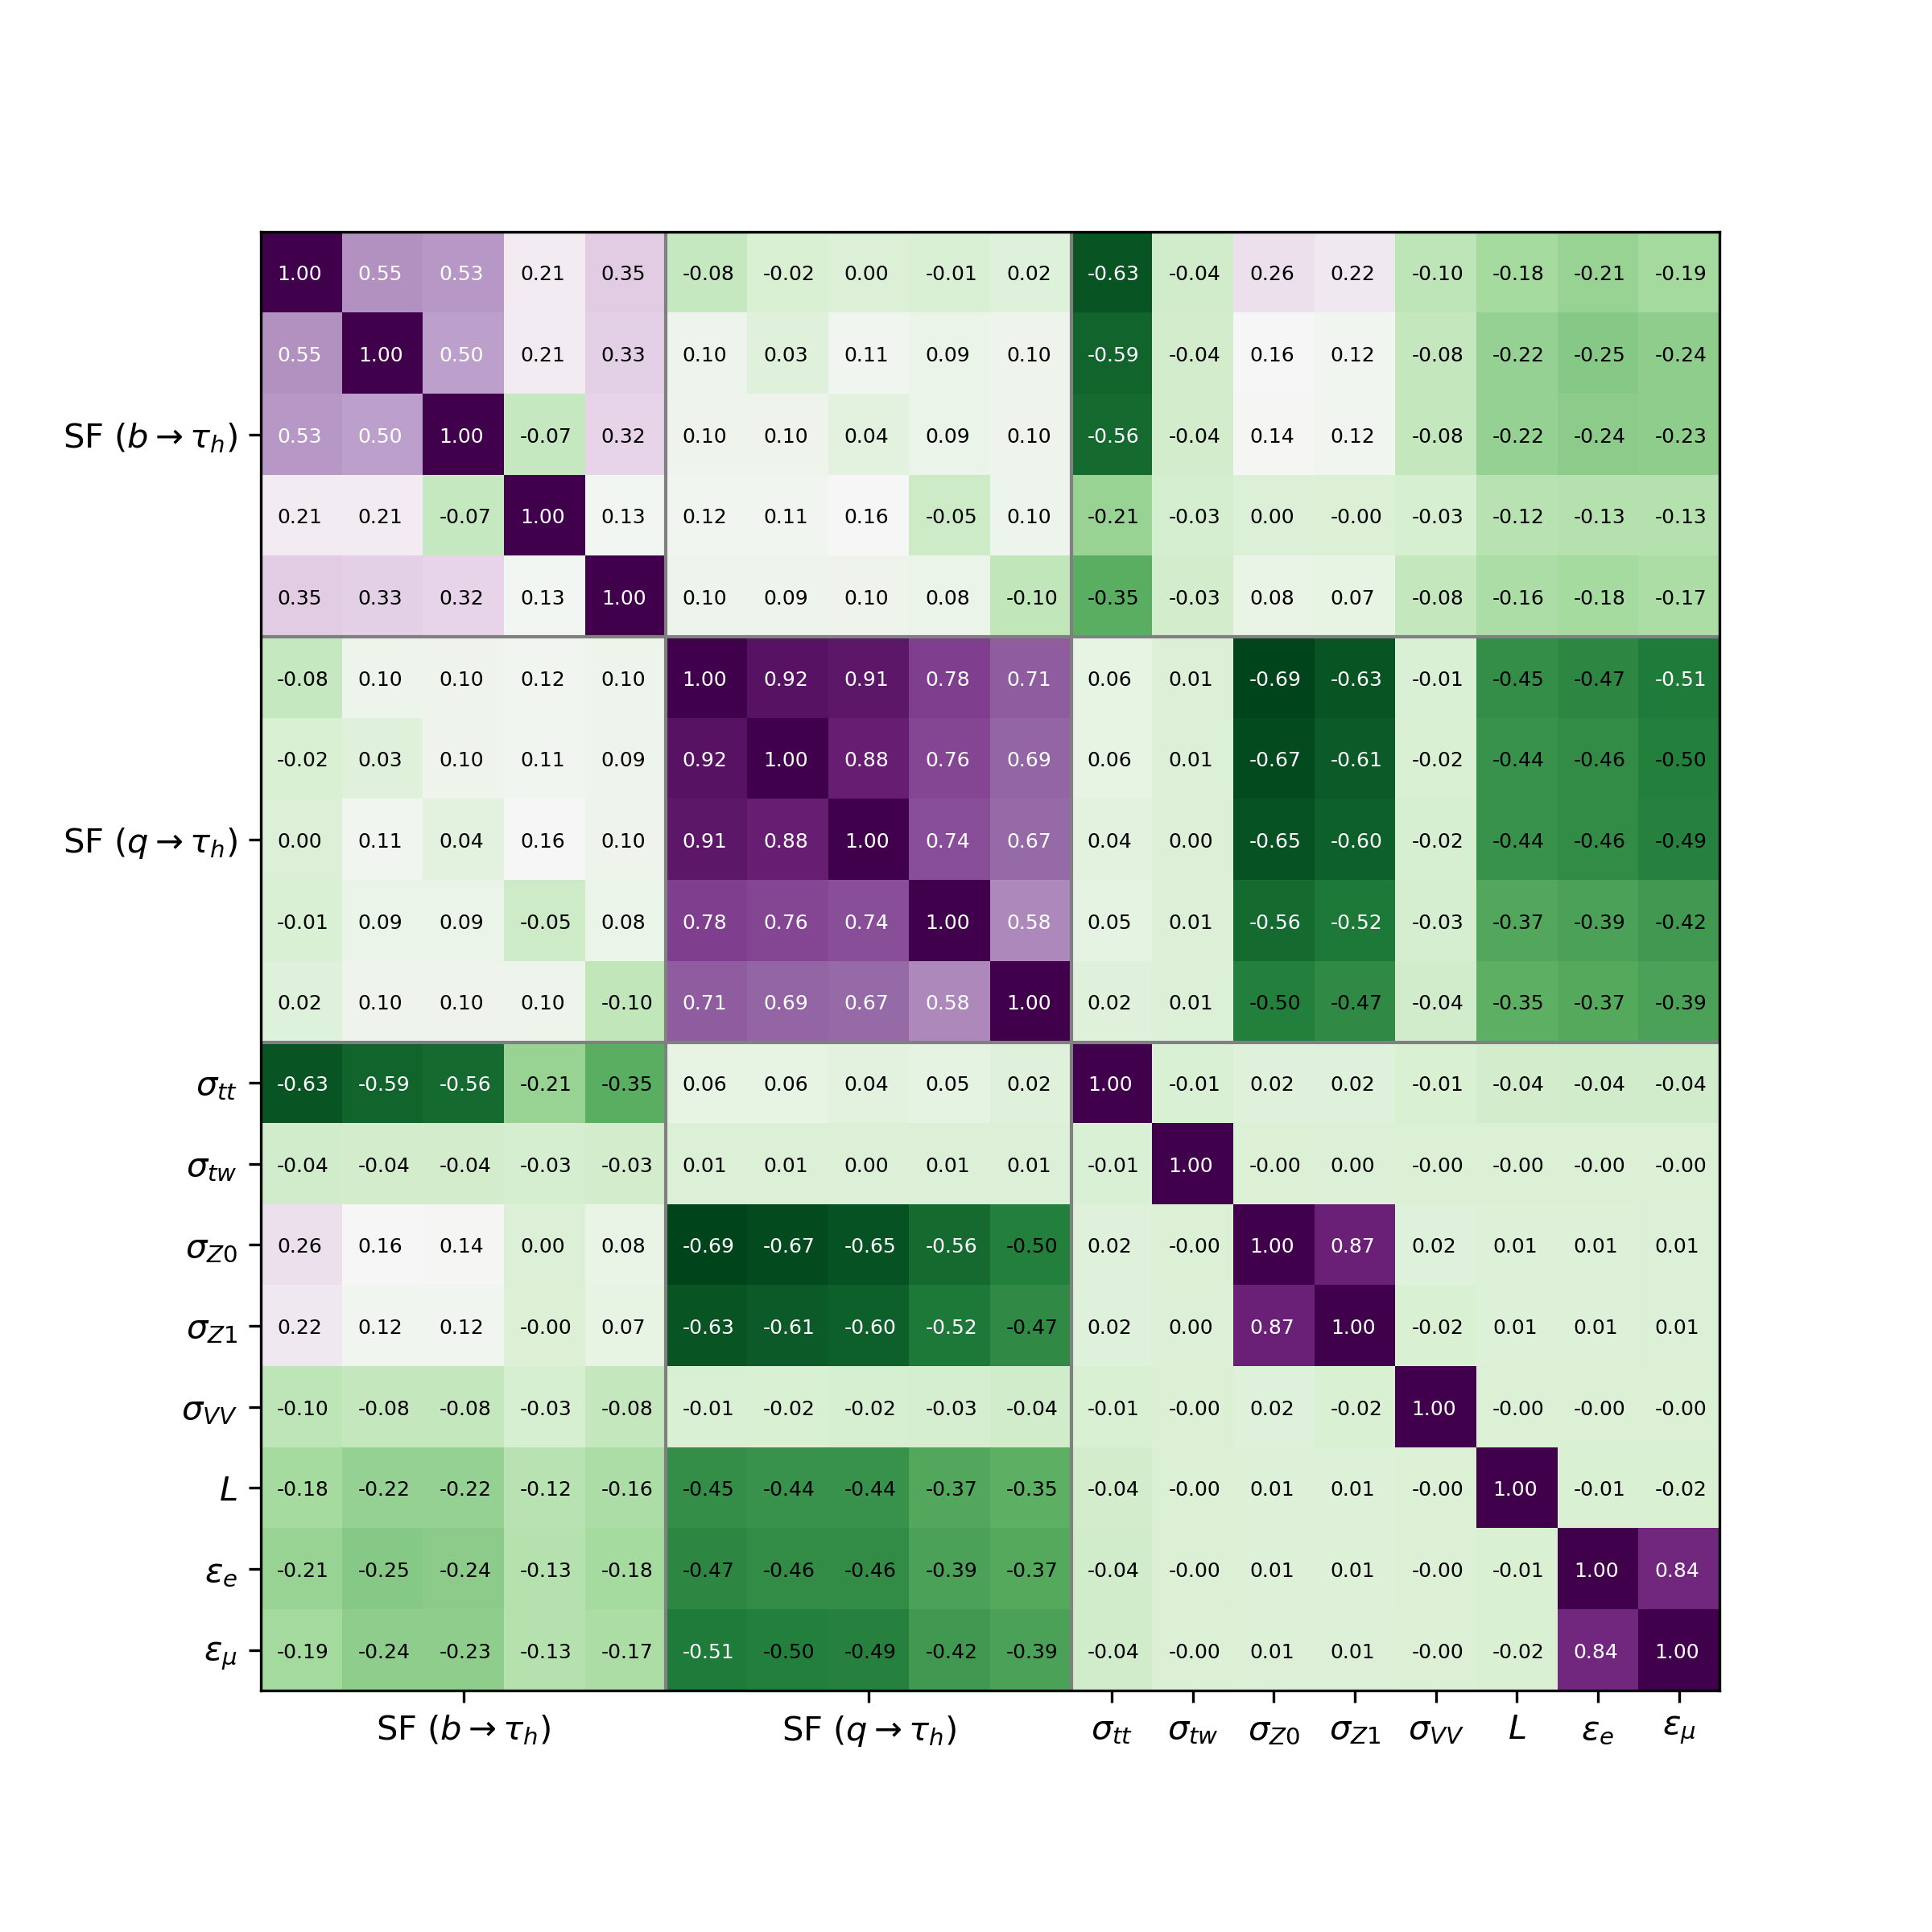
\includegraphics[width=0.49\textwidth]{chapters/Analysis/sectionCalibration/figures/jetToTauh/corr2_lltauTight_splitJetFlavor.png}
    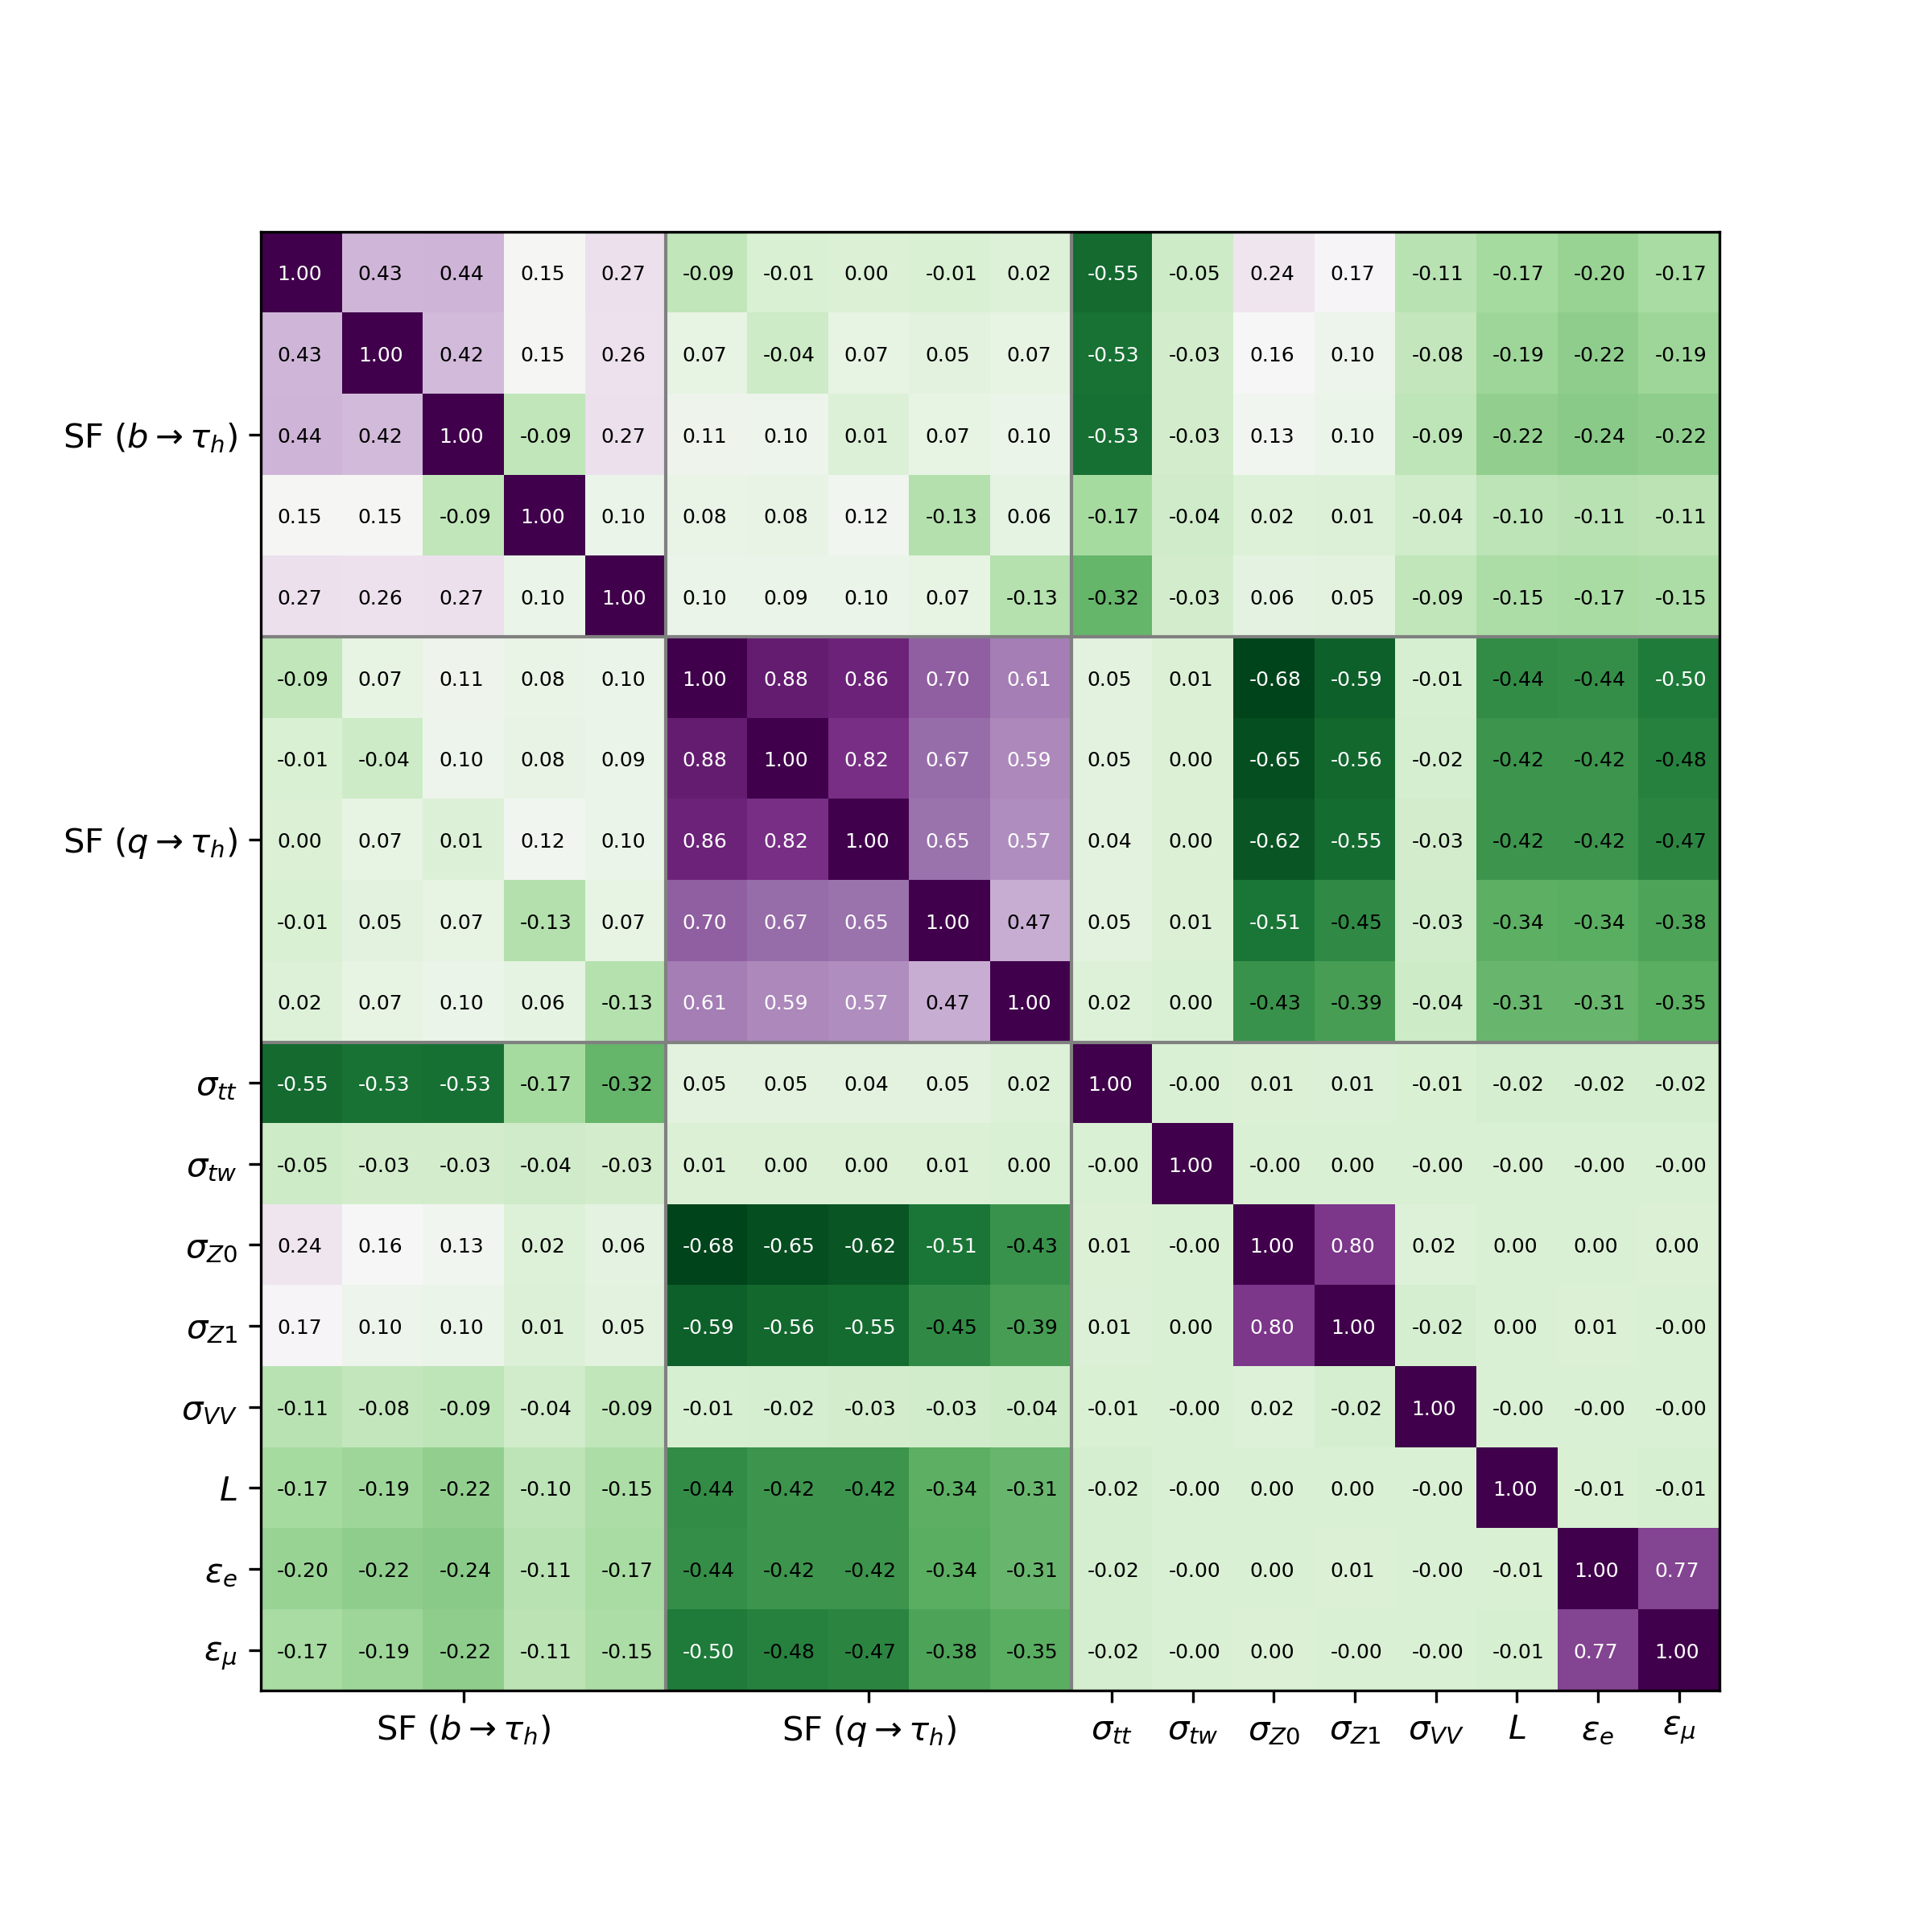
\includegraphics[width=0.49\textwidth]{chapters/Analysis/sectionCalibration/figures/jetToTauh/corr2_lltauVTight_splitJetFlavor.png}
    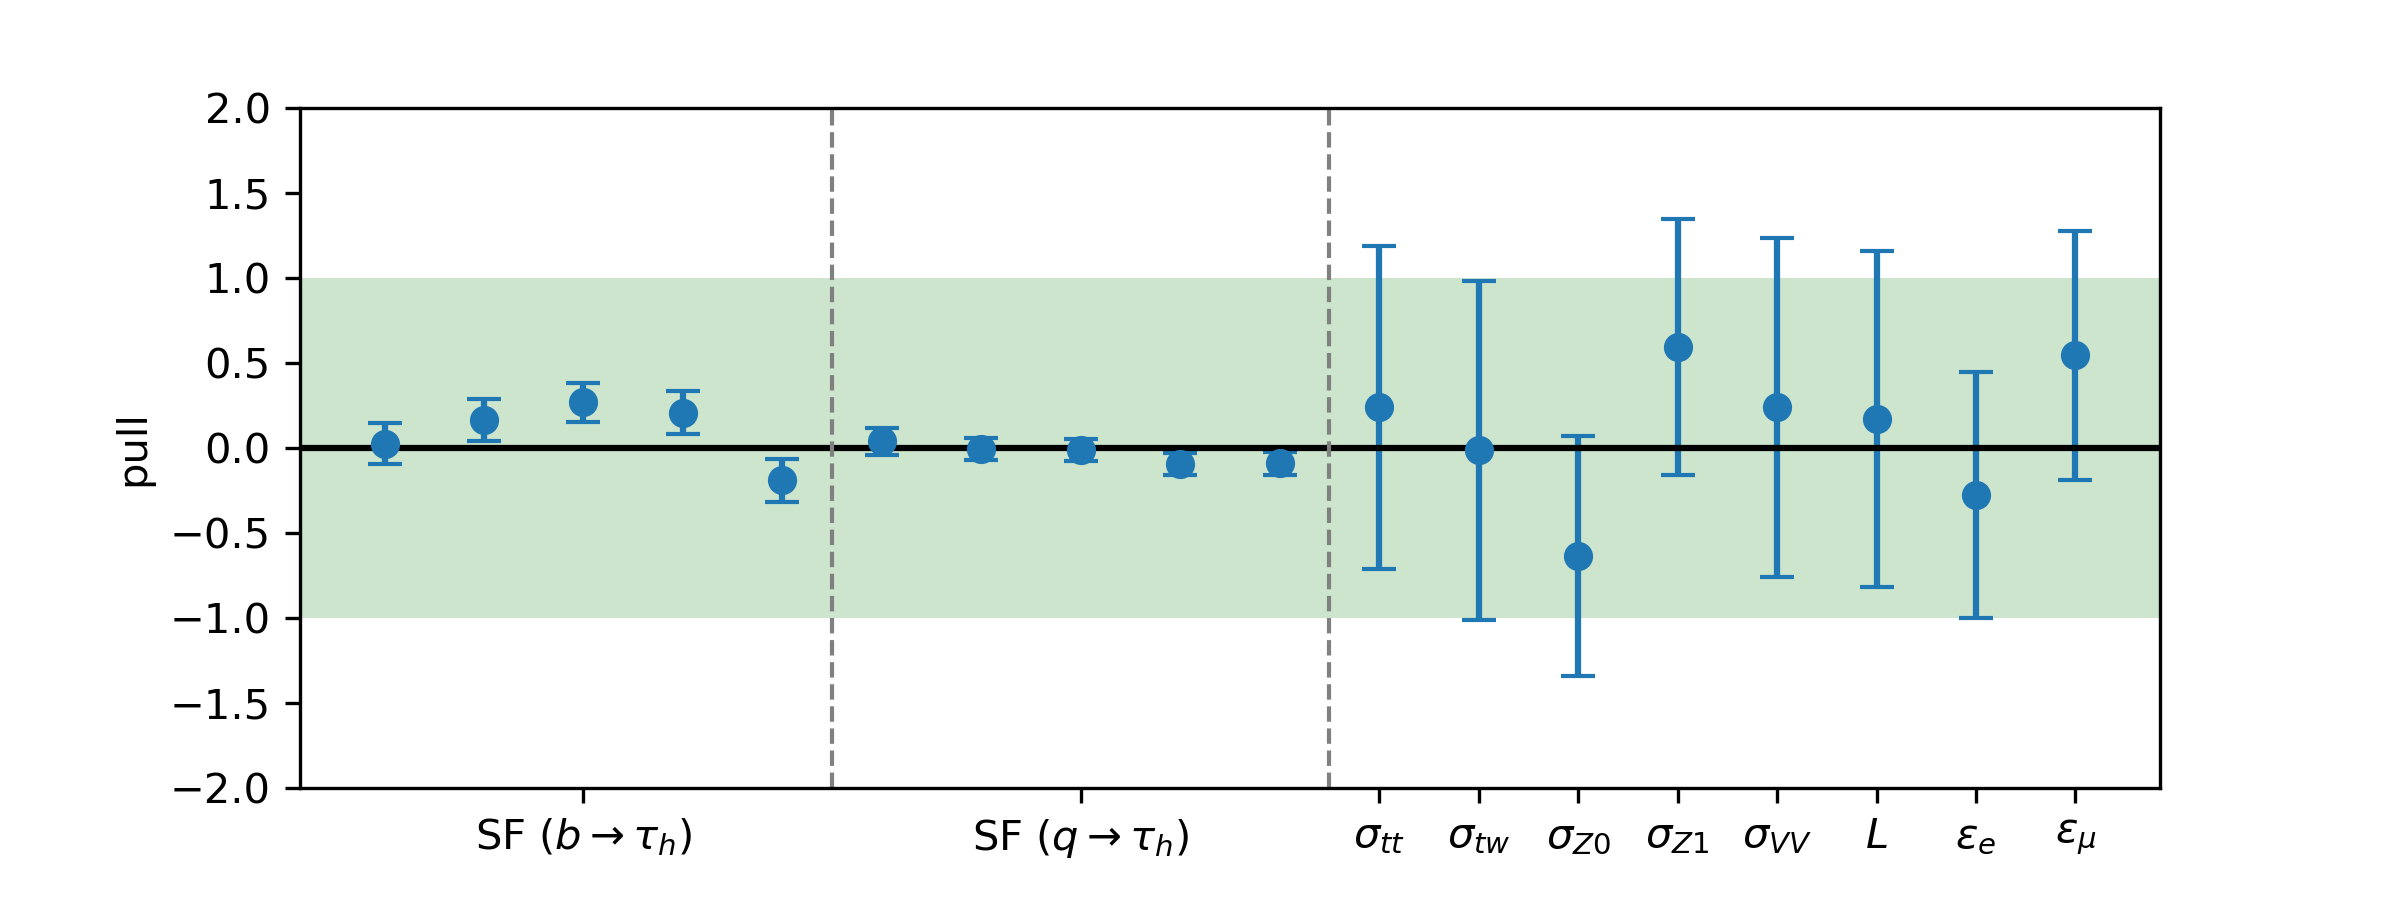
\includegraphics[width=0.49\textwidth]{chapters/Analysis/sectionCalibration/figures/jetToTauh/pull2_lltauTight_splitJetFlavor.png}
    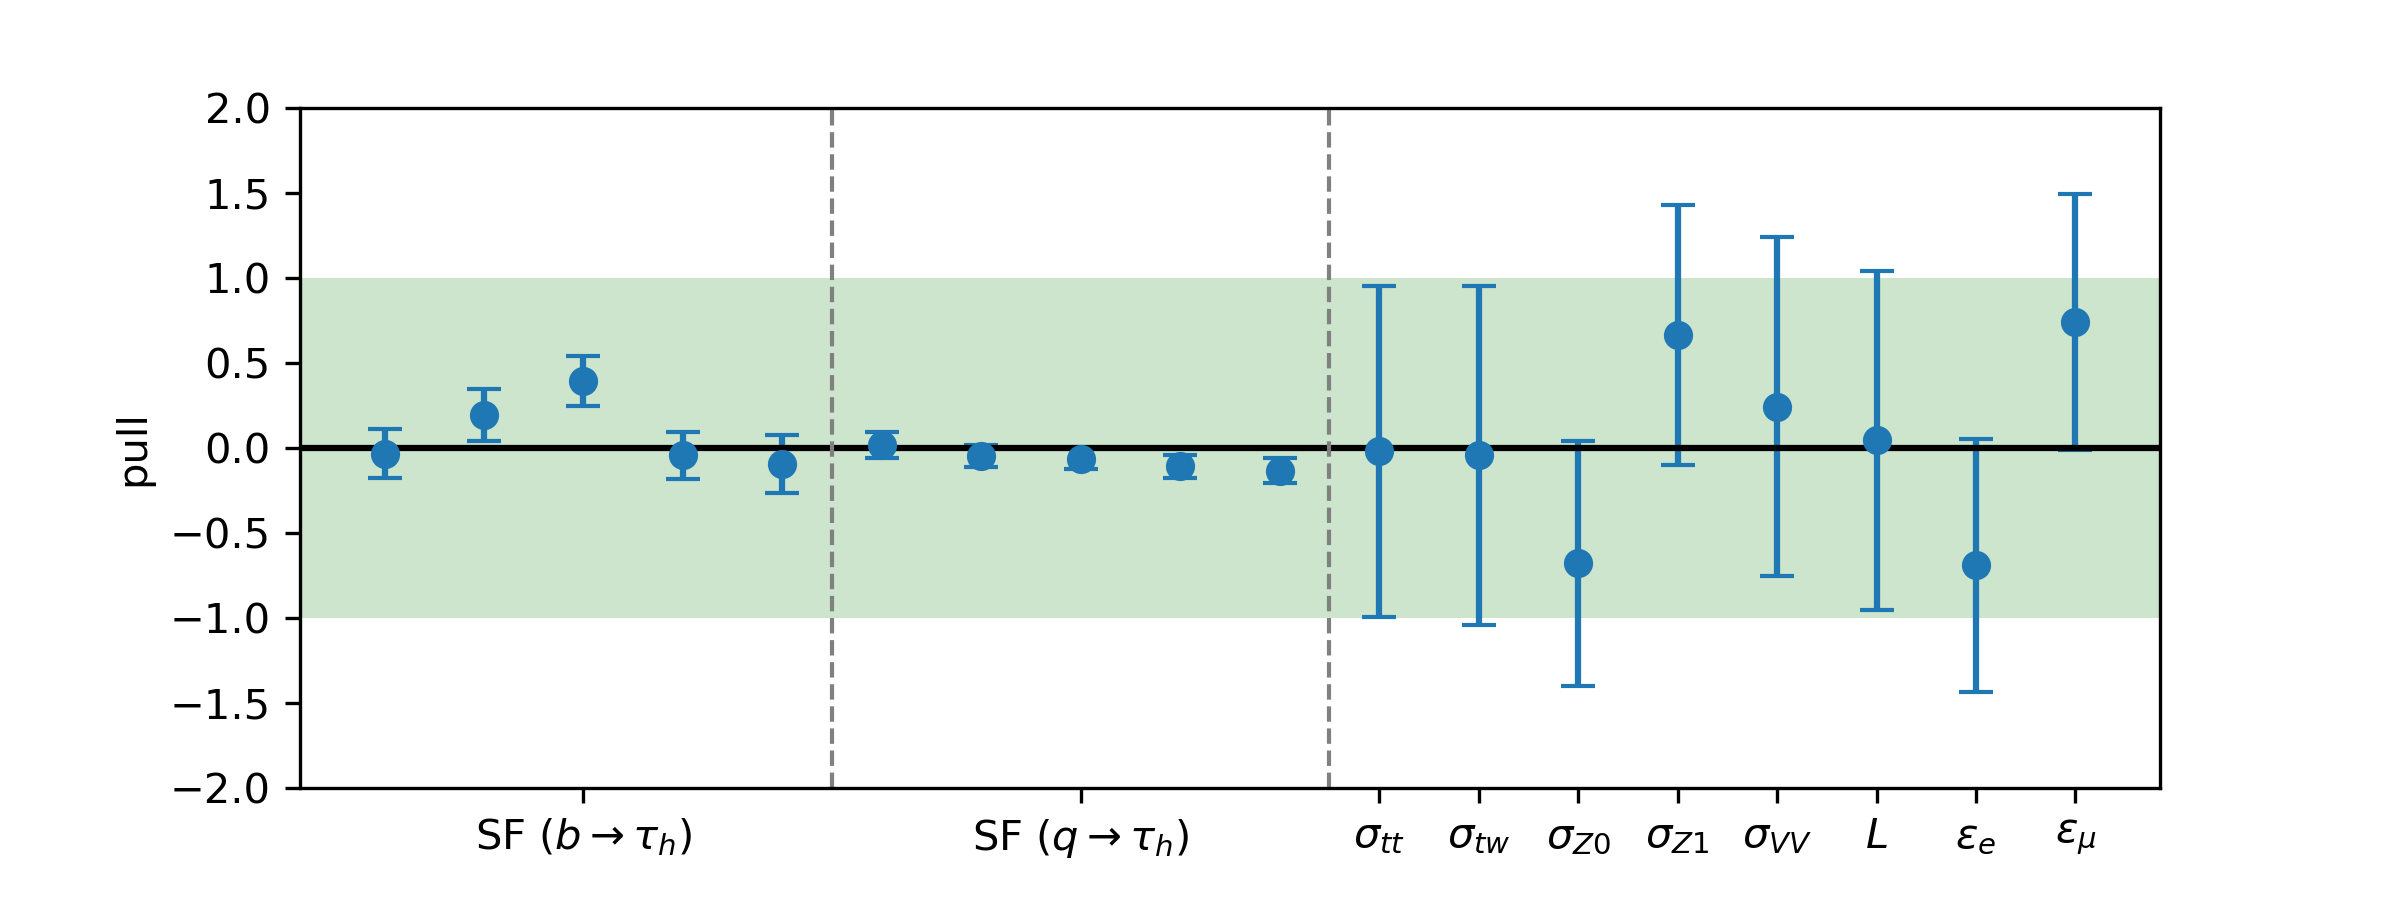
\includegraphics[width=0.49\textwidth]{chapters/Analysis/sectionCalibration/figures/jetToTauh/pull2_lltauVTight_splitJetFlavor.png}
    \caption{The correlation matrix and the pulls of the fitting parameters for Tight (\emph{left}) and Very Tight (\emph{right}) \PGth working point. }
    \label{fig:analysis:calibration:takeTauID_result}
\end{figure}
In the \BWl measurement, to correct the potential mis-modeling of $j\to \PGth$ in the simulation, the origins of selected hadronic taus in the \cet and \cmt channels are tagged with the gen-level truth in the simulated events. The approach of tagging \PGth origins is the same as described here. Based on the \PGth origins, corresponding scale factor in Table~\ref{tab:analysis:calibration:takeTauID_result} is applied to reweight the simulated event.

\FloatBarrier




\subsection{Corrections for b Tag Efficiency and Mistag Probability}
\label{sec:analysis:calibration:btag}
To account for differences of the \PQb tag efficiency in data and simulation, a method that modifies the \PQb tag status of a jet is adopted in the simulation. In the method, the status is modified based on a set of data-to-simulation scale factors $f_{\epsilon}$ derived by the \PQb tag and vertex (BVT) POG, and the efficiencies for simulation $\epsilon$ measured independently in this section.  The method of the \PQb tag correction for simulation works as follows:
\begin{enumerate}
    \item Jets are identified as originating from the decay of a \PQb quark, \PQc quark, or ``light" parton (\PQu,\PQs,\PQd,\Pg) from generator truth information. Depending on the parton flavor and jet \pt, the appropriate scale factor $f_{\epsilon}$ and efficiency from simulation $\epsilon$ are looked up from a map.
    \item If $f_{\epsilon} < 1$, then a \PQb tagged jet is downgraded to a non-b tagged jet with probability $p = 1 - f_{\epsilon}$. If it is not \PQb tagged, nothing is changed.
    \item If $f_{\epsilon} > 1$, then a non-\PQb tagged jet is upgraded to a \PQb tagged jet with probability $p = \frac{1 - f_{\epsilon}}{1 - \frac{1}{\epsilon}}$. If it is already \PQb tagged, its status is unchanged.
\end{enumerate}



The measurement of the \PQb tag efficiency in simulation $\epsilon$ relies on knowing the flavor of the parton that gives rise to the jet.  This is done with official CMS tools that assign a jet flavor based on the characteristics of the quark and gluon content of a jet~\cite{twiki:jet_mc_flavor}.  The efficiencies are measured for the case of \PQb, \PQc, and light (\PQu,\PQs,\PQd,\Pg) flavor jets, and as a function of the jet \pt.  That is,
\begin{equation}
    \epsilon(\pt, \mathrm{flavor}) = \frac{ N_{\mathrm{pass}}(\pt, \mathrm{flavor})} {N(\pt, \mathrm{flavor})},
\end{equation}
\noindent where the numerator is the number of jets passing the \PQb tag working point, and the denominator is the total number of jets considered. These quantities are measured in both \ttbar and \PZ plus jet samples. The CSVv2 discriminator value for the two samples are shown in figures~\ref{fig:analysis:calibration:btag_csvv2} for the three jet flavor categories. The efficiency measurement uses the middle working point of CSVv2 discriminator, the same as the selection in the measurement of \PW branching fraction. The result of \PQb tagging efficiencies is shown in figure~\ref{fig:analysis:calibration:btag_eff}.  There is some level of disagreement between the two samples for the \PQb quark jets that likely could be attributed to the \ttbar sample being generated with an NLO generator (\POWHEG) and the \PZ plus jet sample being generated with a LO generator (\MADGRAPH). The efficiencies from \ttbar sample is used for the \PQb tag correction. The events used for the selection require at least muon passing our analysis requirements, and the four leading \pt jets are considered in the measurement.
\begin{figure}[h!]
    \centering
    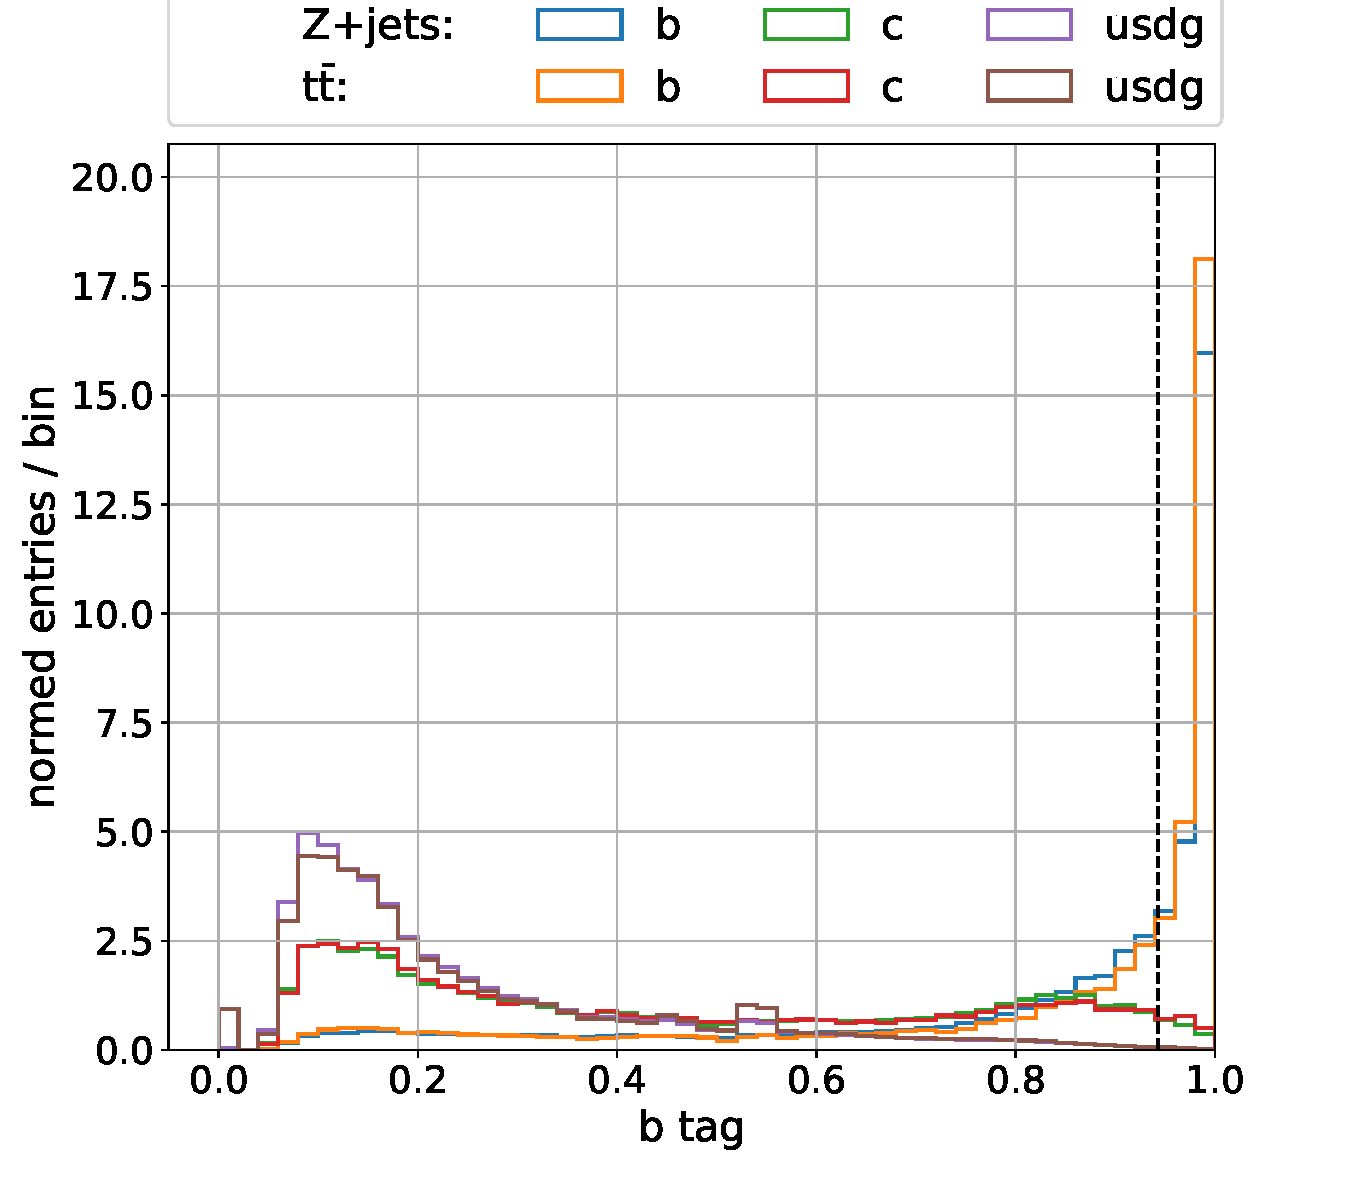
\includegraphics[width=0.45\textwidth]{chapters/Analysis/sectionCalibration/figures/btag/bmva_mc.pdf}
    \caption{Distribution of the \PQb tag score of the \PQb, \PQc and light quark jets in the \zjets and \ttbar simulated dataset.      
    \label{fig:analysis:calibration:btag_csvv2}}
\end{figure}
\begin{figure}[h!]
    \centering
    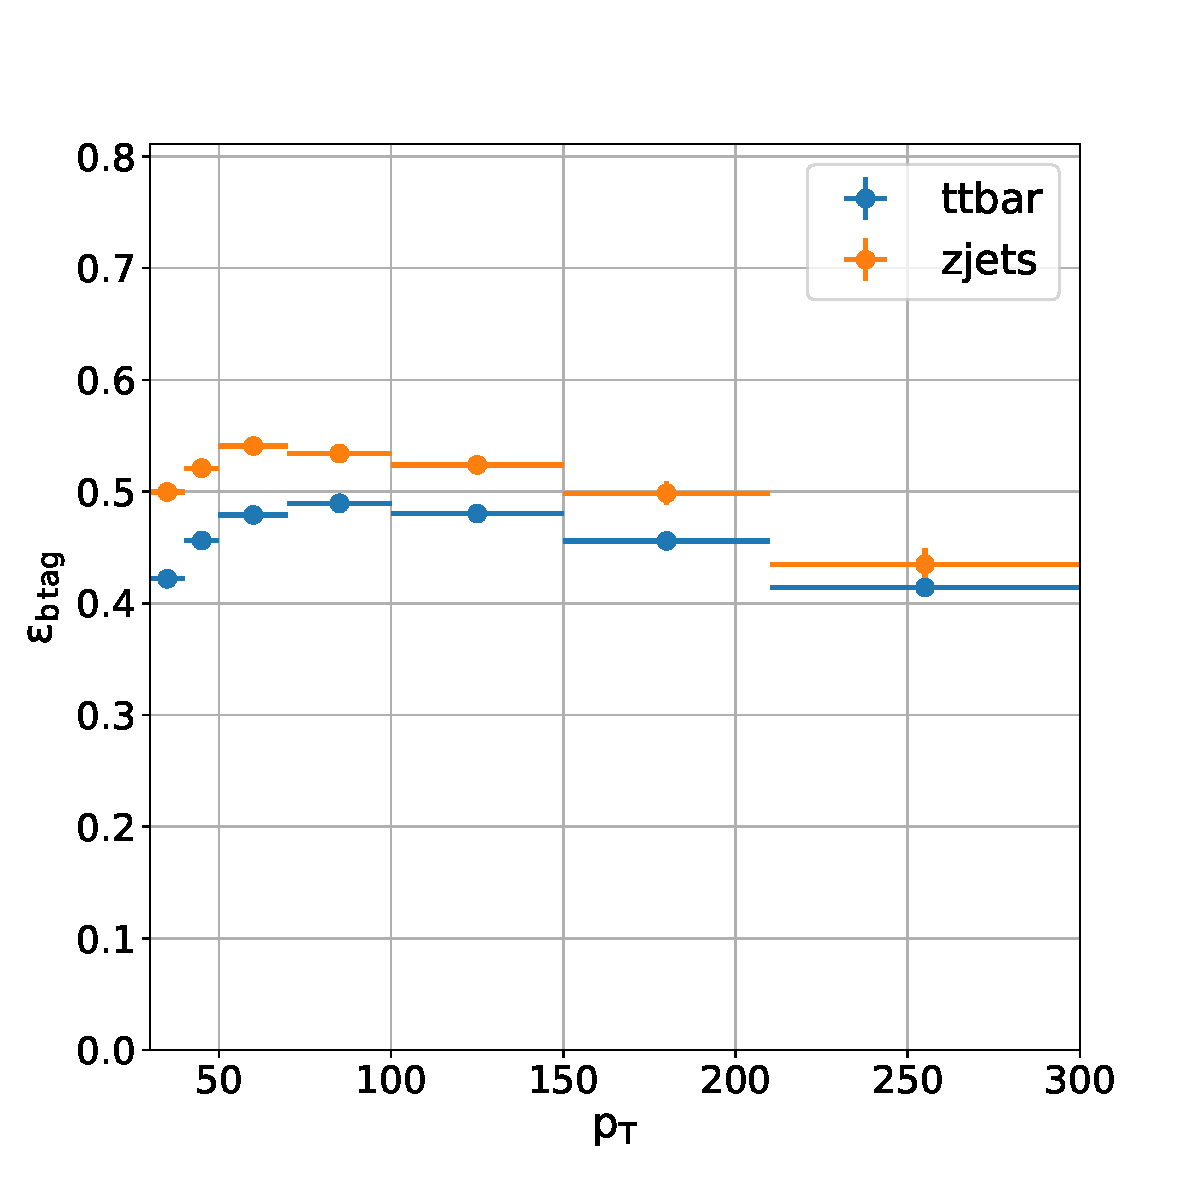
\includegraphics[width=0.3\textwidth]{chapters/Analysis/sectionCalibration/figures/btag/bmva_mceff_vs_pt_b}
    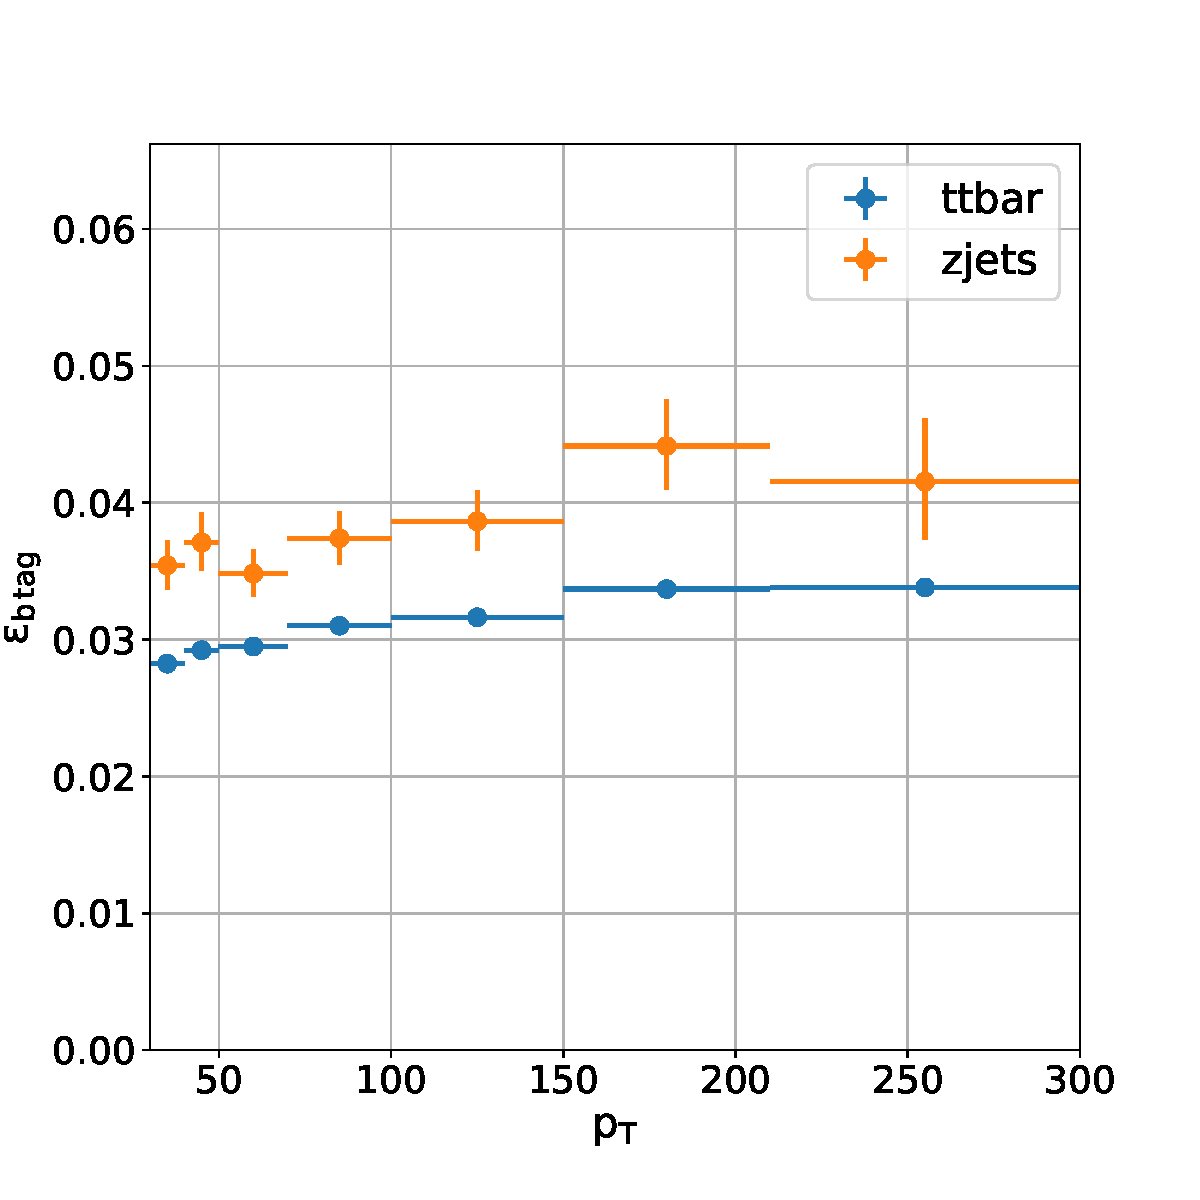
\includegraphics[width=0.3\textwidth]{chapters/Analysis/sectionCalibration/figures/btag/bmva_mceff_vs_pt_c}
    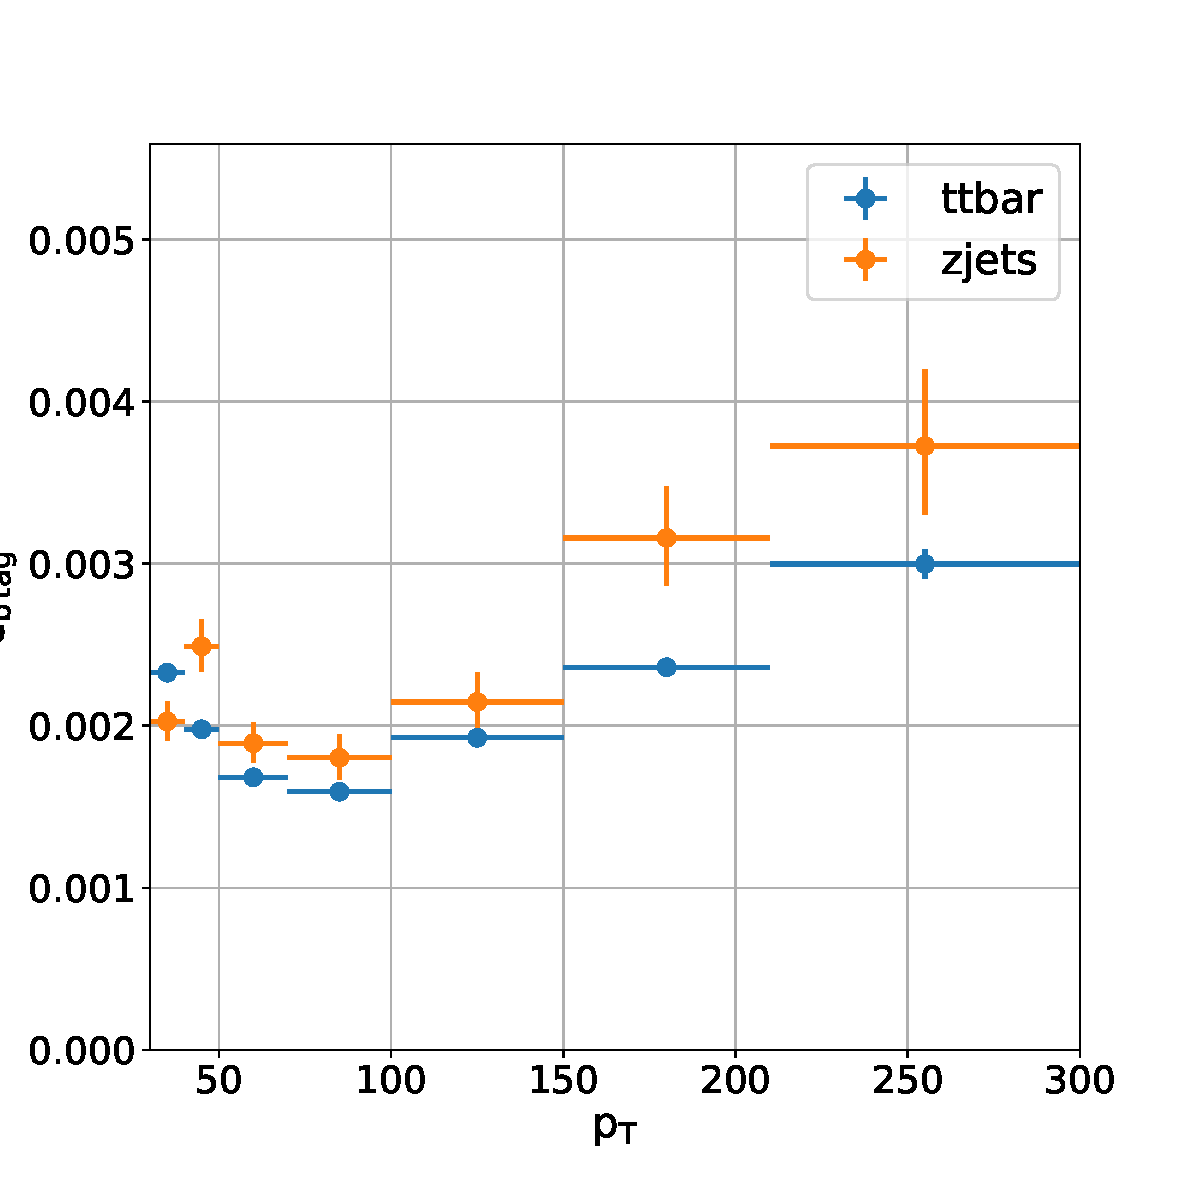
\includegraphics[width=0.3\textwidth]{chapters/Analysis/sectionCalibration/figures/btag/bmva_mceff_vs_pt_usdg}
    \caption{The \PQb tag efficiencies for jets originating from \PQb quark (\emph{left}), \PQc quark (\emph{middle}), and light quark (\emph{right}).
    \label{fig:analysis:calibration:btag_eff}
    }
\end{figure}
\FloatBarrier








